%% This document gives an example on how to use the ntnubachelorthesis
%% LaTeX document class.
%% Use oneside for PDF delivery and twoside for printing in a book style
%% use language english, norsk, nynorsk and one of the following shortenings
%%  ``BSP'' Bachelor i Spillprogrammering,\\
%%  ``BRD'' Bachelor i drift av nettverk og datasystemer,\\
%%  ``BIS'' Bachelor i Informasjonssikkerhet,\\
%%  ``BPU'' Bachelor i Programvareutvikling, \\
%%  ``BIND'' Bachelor i Ingeniorfad - data, \\
%%  ``BADR'' Bachelor i drift av datasystemer, \\
%%  ``BIT'' Bachelor i informatikk, \\
%%  ``BABED'' Bachelor i IT-støttet bedriftsutvikling.
%%   for example \documentclass[BIS,norsk,twoside]{ntnuthesis/ntnubachelorthesis}

\documentclass[BIS,norsk,oneside]{ntnuthesis/ntnubachelorthesis}

\usepackage{csvsimple}
\usepackage{booktabs}
\usepackage{gnuplottex}
\usepackage[T1]{fontenc}
\usepackage[utf8]{inputenc}     % For utf8 encoded .tex files because...
\usepackage[norsk]{babel}       % For Norwegian labeling
\usepackage{graphicx}           % For inclusion of graphics
\PassOptionsToPackage{hyphens}{url}
\usepackage{url}
\usepackage{hyperref}    % For cross references in pdf
\usepackage{tabularx}
\usepackage[table]{xcolor}
\usepackage{colortbl}
\usepackage{placeins}
\usepackage{pdfpages}
\usepackage{enumitem}
\usepackage{multirow}
\usepackage{lscape}
\usepackage{bigstrut}
\usepackage{verbatim}
\usepackage{float}
\usepackage{subfig}


\definecolor{darkgreen}{rgb}{0,0.5,0}
\definecolor{darkred}{rgb}{0.5,0.0,0}

\lstset{        basicstyle=\ttfamily,
                keywordstyle=\color{blue}\ttfamily,
                stringstyle=\color{darkred}\ttfamily,
                commentstyle=\color{darkgreen}\ttfamily,
}


%Typesetting of C++
\newcommand{\CPP}[0]{{C\nolinebreak[4]\hspace{-.1em}\raisebox{.1ex}{\small\bf +\hspace{-.1em}+\ }}}



%\newcommand{\comment}[1]{\textcolor{blue}{\emph{#1}}}  %% use of the colour and you can see how to use commands with parts \comment{so what}

%% The class files defines these two
%% \newcommand{\NTNU}{Norwegian University for Science and Technology} %

% you can create you one #define like structures using the \newcommand feature
% you can change behaviour using \renewcommand

\newcommand{\com}[1]{{\color{red}#1}} % supervisor comment
%\renewcommand{\com}[1]{} %remove starting % to remove supervisor comments
% This will appear in text \com{Lecuters comment} and be visible unless you uncomment
% the renewcommand line.

\newcommand{\todo}[1]{{\color{green}#1}} % items to do
%\renewcommand{\todo}[1]{} %remove starting % to remove items to do

\newcommand{\n}[1]{{\color{blue}#1}} % other comment
%\renewcommand{\n}[1]{} %remove starting % to remove notes

\newcommand{\dn}[1]{} % add the d to a note to say that you have finished with it.

\newcommand{\gj}{NTNU i Gj\o{}vik}


% Norwegian Characters,  needs the {} or to be separate from the next letters
% \o{}   \aa{}   \ae{}   so at the end of a word you can use \o  \aa   \ae
% \O{}   \AA{}   \AE{}   you can also just leave a space and latex will remove it
%    eg, NTNU i Gj\o vik  or NTNU i Gj\o{}vik


\graphicspath{ {bilder/} }

\begin{document}

\thesistitle{A case study on the use of root cause analysis in information security}
\thesisshorttitle{Rotårsaksanalyse for informasjonssikkerhet} % use this if you have a very long title and want something shorter on the header pages
\thesisauthor{Thomas Havnegjerde Huse}
\thesisauthorA{Philip Brugmans Nyblom}
\thesisauthorB{Ole Martin Søgnen}
\thesisauthorC{Fredrik Løvaas Theien}
\thesissupervisor{Tom Røise}
%\thesissupervisorA{john smith} %second supervisor

%\thesisOppgaveNo{9}

\nmtkeywords{Root Cause Analysis, Information Security Management, Case studies}
\nmtdesc{Common approach for information security management is either risk management or incident response. Root cause analysis (RCA) differs from these by identifying root causes and removing them. Since the approach is not often used in information security, one of our topics is to determine how well this approach works. To accomplish this, we looked at three cases tackling various aspects of information security.  The cases were as following: illegal filesharing at NTNU, compromised accounts at NTNU and misuse of NTNU’s resources to mine cryptocurrency. RCA is a collection of various methodologies and tools, however this report follows the methodology and tools presented in ``Root Cause Analysis: Simplified Tools and Techniques’’ \cite{RCA}. The results from the first case shows that it is largely the lack of availability that is the main reason for why students choose to download. In the case about compromised accounts we discovered that poor training and insufficient access control were the main causes. The reasons for why people chose to abuse NTNU’s resources for cryptomining can be attributed to the ambiguities in the IT Policy of NTNU, as well as low priority from the Digital Security Section. Following the completion of the three cases, it was concluded that the methodology works well, but some tools works better than others. Therefore, the report also includes a guideline for using RCA in information security - written based on our experiences from this bachelor project.}

\nmtoppdragsgiver{Seksjon for Digital Sikkerhet, NTNU}
\nmtcontact{Gaute Wangen, gaute.wangen@ntnu.no, +47 907 08 338}


\thesisdate{\ntnubachelorthesisdate}
\useyear{16.05.2018}

\nmtappnumber{11} %numebr of appendixes
\nmtpagecount{} %currently auto calculated but might be wrong




\thesistitleNOR{En case-studie på bruk av rotårsaksanalyse innen informasjonssikkerhet}
\nmtkeywordsNOR{Rotårsaksanalyse, Informasjonssikkerhetsstyring, Case-studier}
\nmtdescNOR{Vanlig tilnærming til informasjonssikkerhetsstyring er gjennom risikostyring og hendelseshåndtering. Rotårsaksanalyse (RCA) skiller seg fra disse ved å gå i dybden på problemet og fjerne det ved rota. Siden denne tilnærmingen er lite brukt i informasjonssikkerhet, er en av våre problemstillinger å utrede hvor godt det fungerer. Tilnærmingen til dette var gjennom tre caser som omhandler ulike aspekter ved informasjonssikkerhet. Disse var å undersøke rotårsaken til: ulovlig fildeling ved NTNU, kompromitterte kontoer ved NTNU og misbruk av NTNU sine ressurser til utvinning av kryptovaluta. RCA består av forskjellige metoder og tilnærminger, men denne rapporten tar utgangspunkt i boken ``Root Cause Analysis: Simplified Tools and Techniques’’ \cite{RCA}. Resultatene fra første case viser at det er i stor grad tilgjengeligheten på tjenester som har noe å si for hvorfor de laster ned. I caset om kompromitterte kontoer viser vår undersøkelse at det er en kombinasjon av dårlig opplæring og utilstrekkelig tilgangskontroll som er rotårsakene. Grunnen til at folk velger å misbruke NTNU sine ressurser til kryptoutvinning kan tilskrives uklarheter i IT-reglement, samt lav prioritering fra Seksjon for Digital Sikkerhet. Etter utføringen av de tre casene ble det konkludert med at metodikken fungerer bra, men at noen verktøy fungerer bedre enn andre. Rapporten inkluderer derfor også en veileder for bruk av RCA innen informasjonssikkerhet – skrevet på bakgrunn av erfaringer fra dette bachelorprosjektet.}

 % this is the file which contains all the details about your thesis

\makefrontpages % make the frontpages

\chapter*{Forord} %the * means do not give the chapter a number
\label{kap:forord}



\tableofcontents
\addtocontents{toc}{\protect\setcounter{tocdepth}{1}}
\listoffigures
\listoftables

\chapter*{Akronymer og begreper}
\label{kap:akronymer}

\section*{Akronymer}
\begin{description}
    \item[RCA] står for Root Cause Analysis, og er en metode for problemløsning.
    \item[ROS] står for Risiko- og sårbarhetsanalyse, og er en metode for å analysere risikoer og innføre tiltak for å føre dem ned til et akseptabelt nivå.
    \item[HPC] står for High Performance Computing, og er gjerne snakk om en regneklynge med høy ytelse, også kjent som en superdatamaskin.
    \item[BYOD] står for Bring Your Own Device, og innebærer alle enheter du tar med deg til jobb eller skole og bruker der.
    \item[DNS] står for Domain Name System og er en tjeneste som brukes for å oversette mellom domenenavn og IP-adresse på internett.
    \item[DHCP] står for Dynamic Host Configuration Protocol, og brukes for å dynamisk tildele IP-adresser på en nettverk etter behov.
    \item[ISMS] står for Information Security Management System, og er et system for å behandle og sette krav til ulike aspekter ved informasjonssikkerhet.
    \item[IAM] står for Identity and Access Management, og er et system som behandler og autoriserer dine autentiseringsdata. Brukes også til å sette krav til passord. 
    \item[SOC] Security Operation Center
    \item[2FA] står for to-faktor autentisering og brukes når man snakker om to autentiseringsfaktorer, som for eksempel passord og kodebrikke. 
\end{description}


\section*{Begreper}
\begin{description}
    \item[Aktiva] er et regnskapsmessig uttrykk for eiendeler eller rettigheter som har formueverdi.
    \item[Case] er en enhet, og brukes gjerne som en case-studie, som betyr studie av en enhet eller et tilfelle.
    \item[Signifikans] er et begrep som brukes for å beskrive sannsynligheten for at noe er et resultat av tilfeldigheter \cite{wiki:sig}.
    \item[Konfidensinterval] er en måte å angi feilmarginen av en måling eller en beregning på. Et konfidensintervall angir intervallet som med en spesifisert sannsynlighet inneholder den sanne (men vanligvis ukjente) verdien av variabelen man har målt \cite{wiki:konfidens}.
    \item[Peer-to-peer] er en betegnelse på en måte å organisere ressursdeling på. I denne rapporten snakker vi spesifikt om fildeling. 
    \item[Symptom] brukes i denne rapporten om en indikasjon på at et problem eksisterer. Et symptom kan i denne sammenhengen være notifikasjoner om brudd på opphavsrett, tap av omløpsmidler eller sikkerhetsvarsler. 
\end{description}
%\chapter*{Kortfattet sammendrag}
\label{kap:kortfattet}

\chapter{Introduksjon}
\label{kap:introduksjon}
Dette kapittlet handler om hvordan dette prosjektet ble til. Vi gir en kort beskrielse av bakgrunnen til prosjektet. Vi presenterer deretter problemstilling med forskningsspørsmål. Vi beskriver også vår motivasjon for oppgaven, rammer som var forhåndsbestemte og avgrensninger vi satt underveis. Helt til slutt inneholder dette kapittelet en oversikt over ønsket mål med dette prosjektet og kort oversikt over hva rapporten inneholder.


\section{Bakgrunn og introduksjon}
\label{sec:bakgrunn}
Root Cause Analysis, RCA, er en metode for problemløsning som brukes for å identifisere rotårsaken til et problem. RCA er et lite brukt verktøy innen informasjonssikkerhet, men er av økende betydning. Vanlig tilnærming til informasjonssikkerhetsstyring er å utføre en risiko-og sårbarhetsanalyse (ROS-analyse) for så å gjennomføre tiltak som fører risikoene til et akseptabelt nivå. En annen hyppig brukt tilnærming er hendelseshåndtering der en planlegger hvordan det skal responderes på hendelser etter de er inntruffet. Rotårsaksanalyse skiller seg fra disse ved å gå i dybden på problemet, kartlegge hva slags rotårsaker som står bak, og innføre tiltak for å fjerne disse helt. 

Vi tar for oss i denne oppgaven forskjellige verktøy som blir brukt innenfor RCA og se hvordan de fungerer innenfor informasjonssikkerhet. 
\section{Problemstilling}

\label{sec:problemstilling}
Hovedproblemstillingen for dette prosjektet er todelt. Den ene delen skal dreie seg om bruk av metode og verktøy for å finne frem til rotårsaken for tre ulike caser. Hvert case omfatter en hendelse eller et problem NTNU har, som de ønsker å eliminere. De tre problemene er som følger: 

\begin{enumerate}
    \item Ulovlig fildeling på universitetsnettet til NTNU
    \item Kompromitterte brukerkontoer ved NTNU
    \item Misbruk av NTNU sine ressurser til utvinning av kryptovaluta
\end{enumerate}

I tillegg til dette har vi en underliggende problemstilling knyttet til alle tre casene hvor vi redegjør for hvordan rotårsaksanalyse kan brukes innenfor informasjonssikkerhet. Denne vurderingen gjøres etter gjennomføring av casene for å se hvordan metoden og verktøyene fungerte. Dette dokumenteres til senere bruk.

Utover de tre casene skal vi bruke dokumentasjon og erfaring fra disse til å utarbeide retningslinjer for gjennomføring av rotårsaksanalyse for informasjonssikkerhet. Dette dokumentet skal inneholde informasjon om metode, fremgangsmåte og dokumentasjon av verktøy som fungerer bra i denne sammenhengen. Dokumentet skal kunne brukes aktivt av fagmiljøet når det skal utføres ytterligere rotårsaksanalyser. Derfor vil retningslinjene inneholde en deler som er fra hovedrapporten, dette dokumentent skal kunne stå for seg selv.

I rapporten ønsker vi å redegjøre følgende forskningsspørsmål:

\begin{itemize}
    \item Hva er rotårsaken til at studenter laster ned opphavsrettsbeskyttet materiale?
    \item Hva er rotårsaken til at brukerkontoer ved NTNU blir kompromittert?
    \item Hva er rotårsaken til misbruk av NTNU sin infrastruktur til utvinning av kryptovaluta?
    \item Hvor godt fungerer rotårsaksanalyse innen informasjonssikkerhet?
    \item Lønner det seg å benytte rotårsaksanalyse i informasjonssikkerhetssammenheng?
    \item Hvilke metoder og verktøy som ofte brukes i rotårsaksanalyse, fungerer best innen informasjonssikkerhet??
\end{itemize}
\section{Motivasjon}
\label{sec:motivasjon}
Oppdragsgiver ønsker å få en bedre forståelse for bruk av rotårsaksanalyse innen informasjonssikkerhet og eliminere problemer tilknyttet oppdragsgivers ansvarsområder. Prosjektet skal bistå til økt forståelse ved å undersøke verktøy- og metodebruk fra RCA innenfor Seksjon for Digital Sikkerhet sitt fagfelt. Prosjektet skal presentere en tiltaksplan som eliminerer noen av problemene oppdragsgiver har i sitt ansvarsområde. En motivasjon er derfor økt tilgang på ressurser i form av arbeidskraft for å løse problemer. 


Motivasjonen vår innebærer et ønske om økt kompetanse knyttet til risikoer og hendelser, og metodebruk for å håndtere disse. Vi ønsket dermed en oppgave som var styringsrelatert fremfor teknisk. Denne oppgaven handlet om noe som for oss var en ny tilnærming til informasjonssikkerhetsstyring. Vi ønsket derfor å være med å vurdere bruken av RCA i informasjonssikkerhet og om det burde benyttes i tillegg til ROS-analyse og hendelseshåndtering. 
\section{Rammer}
\label{sec:rammer}
Her defineres rammene som er satt forhåndsbestemte rammer som er satt. 

\begin{itemize}
    \item Prosjektet var aktiv i peroden 8. januar til 16. mai.
    \item Prosjektet var delt inn i tre hendelser som skulle analyseres
    \item Alle medlemmene i gruppen bor i gjøvik, og nærme skolen. Så det var satt av møter hver dag.
    \item Rapporten ble skrevet i programmet ''ShareLaTeX''
\end{itemize}
\section{Avgrensing}
\label{sec:avgrensing}
Innen rotårsaksanalyse finnes det flere verktøy og metoder, men på grunn av begrenset tid og ressurser avgrenser vi oss til verktøyene og metoden beskrevet i boka ``Root Cause Analysis: Simplified Tools and Techniques - second edition'' av Bjørn Andersen og Tom Fagerhaug \cite{RCA}. Generelt for prosjektet vil vi følge føringer fra Seksjon for Digital Sikkerhet.

\noindent Spesielt for hvert case gjelder:

\textbf{Case 1:}
Caset avgrenses til studenter i Gjøvik som leier studenthybel fra SiT.

\textbf{Case 2:}
Informasjonsinnsamlingen avgrenses til kun 200 personer av de som har blitt kompromittert. 

\textbf{Case 3:}
MÅ LEGGES INN NÅR VI FÅR OPPGAVEN

\section{Prosjektmål}
\label{sec:prosjektmaal}
Målet for prosjektet er å gå i dybden på tre ulike caser som hver omhandler en unik hendelse eller et problem NTNU har. Prosjektmålene deles inn i effektmål og resultatmål.

\subsection{Effektmål}
Effektmålene er det oppdragsgiver ønsker å oppnå med oppgaven og rapporten etter den er utredet og levert.
\begin{itemize}
    \item Eliminere problemene beskrevet i de tre casene helt eller delvis ved implementering av tiltak beskrevet i rapporten
    \item Økt forståelse for bruk av RCA i informasjonssikkerhet
    \item Finne ut hvor fordelaktig det er å bruke RCA i informasjonssikkerhet og hvilke verktøy som fungerer best til dette
\end{itemize}

\subsection{Resultatmål}
Resultatmålene beskriver det prosjektet skal oppnå i det prosjektperioden er over, og oppgaven er utført og levert.

\begin{itemize}
    \item Alle tre caser er utført og har en individuell rapport hver
    \item En oversikt over hovedfunn fra tre caser med RCA
    \item Dokumentere bruk av RCA i informasjonssikkerhet, med forklaringer og konkluderinger av metode og verktøy
    \item Redegjørelse for hvor godt rotårsaksanalyse fungere innen informasjonssikkerhet, og om det lønner seg
\end{itemize}
\section{Organisering av rapporten}
\label{sec:organisering_rapport}
Prosjektrapporten inneholder 7 kapitler i tillegg til vedlegg.


\begin{description}
    \item [Kapittel 1: Introduksjon] inneholder grunnleggende informasjon om prosjektet.
    \item [Kapittel 2: Casebeskrivelser] inneholder detaljert beskrivelse av hvert case vi skal analysere.
    \item [Kapittel 3: Teori] inneholder bakgrunn og teori om rotårsaksanalyse, samt sammenlikning med eksisterende metodikk innen informasjonssikkerhet.
    \item [Kapittel 4: Metode] inneholder beskrivelse av metoden vi benyttet når vi skulle tilnærme oss rotårsaksanalyse av informasjonssikkerhetshendelser. Kapittelet beskriver alle fasene i prosessen, samt verktøyene som ble benyttet i hver fase. 
    \item [Kapittel 5: Resultater] inneholder hovedfunnene i de tre casene vi analyserte.
    \item [Kapittel 6: Diskusjon] inneholder diskusjon om resultatene.
    \item [Kapittel 7: Konklusjon] inneholder oppgavens konklusjon.
\end{description}
\chapter{Casebeskrivelser}
\label{kap:casebeskrivelser}
Oppgavene som blir analysert i denne rapporten er gjort ved hjelp av rotårsaksanalysemetodikk i henhold til ``Root Cause Analysis: Simplified Tools and Techniques - second edition'' av Bjørn Andersen og Tom Fagerhaug \cite{RCA}. Dette for å få en større forståelse for rotårsaksanalyse i sammenheng med det digitale og spesielt da informasjonssikkerhet.

\section{Case 1: Ulovlig fildeling på universitetsnettet}
\label{sec:case_fildeling}
NTNU har ansvar for nettet hos studenthyblene studentene leier fra SiT. Når studenter driver med ulovlig fildeling fra hybelen vil NTNU kunne holdes ansvarlig. Dette er et problem for NTNU, ikke bare i form av skadet omdømme, men det kan også være problematisk hvis opphavsrettshaverne går juridisk til verks. Oppgaven i dette caset er derfor å finne, ved hjelp av rotårsaksanalysemetodikken, rotårsaken til hvorfor studenter laster ned opphavsrettighetsbeskyttet materiale. Det skal også presenteres en tydelig tiltaksplan for å eliminere denne.

\subsubsection{Oversikt over oppgaven}
Advokater til diverse filmselskaper ser etter IP-er til personer som laster ned deres opphavsrettsbeskyttede materiale, og sender disse personene notifikasjoner på e-post. Hver måned får NTNU ca. 150 og 200 unike notifikasjoner om brudd på opphavsretten ved ulovlig fildeling. Vi kan se at dette nummeret går kraftig ned i sommermånedene, som tilsier at studentene er hovedgrunnen til bruddene på opphavsrett. Dersom opphavsrettshaverne begynner å håndheve opphavsretten i brevene de sender, kommer NTNU til å havne i en dårlig posisjon. I dag gjør ikke NTNU noe med de mange brevene de får, grunnet de store mengdene og at det er en fulltidsjobb i seg selv å håndtere dem.

%Ulovlig fildeling foregår som regel ved hjelp av en protokoll som heter BitTorrent som bruker peer-to-peer teknologi. Universitetet har per dags dato ikke lov til å blokkere denne da protokollen også innebærer legitimt bruk. NTNU er eneste internettleverandør til studenthyblene og studenter kan derfor ikke velge hvilken leverandør de ønsker seg.
\section{Case 2: Kompromitterte kontoer}
\label{sec:case_kontoer}
NTNU er et stort universitet med mange ansatte. NTNU er derfor et mål for aktører med ondsinnete hensikter. En av disse er hensiktene er å få tilgang til brukerkontoer. Disse kontoene blir brukt til mye forskjellig. De brukes ofte for spam, innhenting av store mengder forskningsartikler og videre salg. Måten disse kontoene kommer på avveie er uvisst, men noen av hypotesene innebærer phishing og gjenbruk av brukernavn og passord på nettsider som har blitt kompromittert. Vår oppgave i dette caset er å bruke rotårsaksanalyse til å finne og presentere tiltak som eliminerer rotårsaken til at kontoer ved NTNU blir kompromittert.

\subsubsection{Oversikt over oppdraget}
NTNU har siden 2005 fått 5415 kontoer kompromittert. Disse kontoene ble funnet i en stor datadump i desember 2017. Av disse 5415 kontoene var 101 av dem fremdeles aktive. Det vil si at brukernavn og passord fortsatt var gyldige innloggingskredentialer da de ble avdekket. 

Universitetet betaler for tilgang til databaser som inneholder tusenvis av forskningsartikler og andre artikler. 26 av de kompromitterte brukerne ble brukt av utenlandske aktører for å skaffe seg tilgang til forskningsartikler. Konsekvensen ved å ha kompromitterte kontoer som laster ned forskningsartikler er ikke bare at NTNU taper penger, men at NTNU risikerer å bli blokkert fra databasene. Angriperne derimot tjener på å ikke trenge å betale for tilgang til databasene. Et annet punkt som gjør det lukerativt å kompromittere universitetskontoer er at disse kontoene kan bli solgt på nett, der kredentialer behandles som ferskvare. 

Det blir hentet ut flere tusen forskningsartikler på en gang per bruker. Universitetet vet ikke om når det blir hentet ut artikler, eller om det er legitimt bruk av artiklene. De får ofte vite det først når universitetet får beskjed av samarbeidspartnere til NTNU, for eksempel de som tilbyr artiklene. 

\section{Case 3: Misbruk av NTNU sin infrastruktur til utvinning av kryptovaluta}
\label{sec:case_krypto}
Kryptovaluta har kommet mer i nyhetsbildet i det siste. Kryptovaluta er en anonym måte å betale og man kan utvinne kryptovaluta ved hjelp av mining. Miningen kan bli gjort på flere måter, en kan installere et program på pcen eller det man kan mine direkte gjennom browseren med javascript, sistnevnte kan være som erstatning til reklame, eller en ondsinnet måte for nettsider/andre å tjene penger på.




\subsubsection{Oversikt over oppgaven}
Siden november 2017 har mengeden med mining på skolen økt med 8000\%, siden universitetet ikke har lov til å bruke sine ressurser til personlig vinning er dette blitt et stort problem. Grunnen til den økningen er at i 2017 begynte flere å spekulere i kryptovaluta og siden det er et uregulert marked var det veldig store svinginger som igjen førte til at det kom mange flere aktører på banen både som leverandører og spekulanter. 

Oppgaven deles inn i to aktører de som frivillig bestemer seg for å drive med mining og de som får ressursene sine missbrukt til å mine for kriminelle selskaper eller nettsider, der de ikke sier ja til bruk av sine ressurser.

Oppgaven har to spørsmål som må besvares og de er hvorfor og hvordan utvinning av kryptovaluta foregår.
\chapter{Teori og tidligere arbeid}
\label{kap:teori}

\section{Utvalg av faglittertaur}
Rotårsaksanalyse som helhet finnes det masse litteratur om, men metodene er veldig spredt. Innen informasjonssikkerhet finnes det lite litteratur. Vi har valgt boken ``Root Cause Analysis: Simplified Tools and Techniques'' av Fagerhaug og Andersen \cite{RCA} som gir en generell beskrivelse av rotårsaksmetodikken, men ikke spesifikt for informasjonssikkerhet. Vi har i tillegg brukt bacheloroppgave fra 2016 \cite{RCARapport} som så på anvendelsen av rotårsaksanalyse innen informasjonssikkerhet.

\subsection{Hvorfor ble disse valgt?}
Vi valgte boken \cite{RCA} på anbefaling av oppdragsgiver og fordi vi ville se hvor godt den fungerte innen informasjonssikkerhet. Vi ville se hvor godt boka fungerte som en samlet metodikk for rotårsaksanalyse. 

\subsection{Hvordan vi fant frem til disse?}


\section{Teori}
Rotårsaksanalyse er en fremgangsmåte for å finne roten til et problem og eliminere det. RCA analyserer de underliggende faktorene og bruker årsakene til å finne roten til problemet. RCA er en reaktiv prosess som finner svar på problemer basert på skjulte årsaker og deres effekt, istedenfor å undersøke den mest åpenbare årsaken. Det gjør at RCA er ofte komplekst og tidkrevende, men når rotårsaken først er funnet kan løsningene fjerne problemet helt. 

\subsection{Historie}
Det har finnes flere varianter av rotåsaksanalyse opp gjennom tidene, men mannen som er kreditert med å finne opp rotårsaksanalyse er grunnleggeren av Toyota, Sakichi Toyoda. Hans versjon av RCA ble tatt i bruk av Toyota produksjonsprosess i 1958 og ble kalt ``5 Whys''. Som tidligere sagt har RCA forandret seg over tidene for å imøtekomme de forskjellige feltene. Nå brukes RCA som verktøy i flere felter som transport, medisin og luftfart\cite{Teori}. 
    
\subsection{Ulike nivåer av årsaker}
Et problem er som regel ikke et resultat av en årsak, men heller en kombinasjon av flere årsaker på flere forskjellige nivåer. Dette vil si at årsaker påvirker andre årsaker helt opp til det synlige problemet. Årsaker defineres i tre forskjellige grupper: 

\begin{description}
    \item[Symptomer] er ikke å regne som faktiske årsaker, men heller bevis på eksisterende problemer.
    \item[Første-nivå årsak] er årsåker som leder direkte til et problem.
    \item[Høy-nivå årsaker] er årsåker som blir til første-nivå årsaker. Selv om de ikke direkte er årsak til problemmet, skaper høy-nivå årsak lenker i kjeden av årsak-virkningsforholdet som til slutt fører til problemet. Den høyeste nivå årsaken er rotårsaken.  
\end{description}
Noen problemer har flere årsaker som er forbundet av de forskjellige faktorer som kombinert blir til problemet.

\begin{figure}[H]
    \centering
    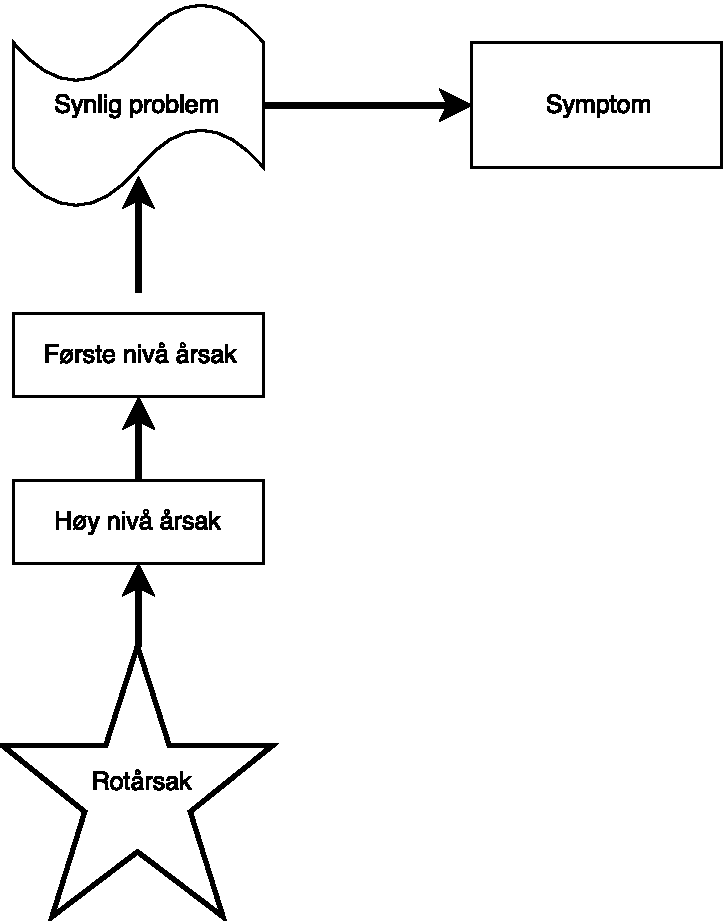
\includegraphics[scale=0.6]{main/bilder/nivaa.pdf}
    \caption[Nivåer av årsaker]{De forskjellige nivåer til problemet}
    \label{fig:nivaa}
\end{figure}

Vi ser fra figuren at rotårsaken er det som setter i gang årsak-virkningskjeden som leder til problemet. 

\subsection{Root Cause Analysis: Simplified tools and techniques}
Denne boken fra 2006 gir en generell beskrivelse av verktøyene og fremgangsmåten til rotårsaksanalyse. 

\subsection{Tidligere arbeid innen informasjonssikkerhet}
I 2016 ga NTNU en bacheloroppgave som innebar bruk av rotårsaksanalyse på tre forskjellige caser \cite{RCARapport}. Oppgaven viste at rotårsakanalyse fungerer i informasjonsikkerhetssammenheng. Vår oppgave skal jobbe videre med å se på hvordan rotårsaksanalyse fungerer i informasjonsikkerhet. OBS: TIL UTBEDRING!

\subsection{Rotårsaksanalyse sammenlignet med risikoanalyse}
En risikoanalyse ser på sannsynlighet for at en trussel kan skje og mulige konsekvenser av dette. Risikoen regnes ut fra sannsynlighet og konsekvens, samt eksisterende kontroller. I risikoanalysen vil dataene brukes til å finne mulige preventive og reaktive tiltak som kan føre riskoen ned på et akseptabelt nivå. Rotårsaksanalyse vil på sin side gjøre en systematisk gjenomgang for å finne de underliggende årsakene til feil eller svikt. En rotårsaksanalyse gjøres etter et problem har oppstått, i motsetning til riskoanalyse som gjøres for å behandle fremtidige situasjoner. 
\chapter{Metode}
\label{kap:metode}
Vår tilnærming til anvendt rotårsaksanalyse i dette prosjektet er gjennom tre caser som omhandler informasjonssikkerhet. Utførelse av rotårsaksanalyse kan gjøres på ulike måter, men grunnstrukturen er ofte lik. Det handler i bunn og grunn om problemløsning. I tillegg til å analysere casene skal bruken av metoden vurderes ut i fra hvor godt den fungerer innen informasjonssikkerhet. Påfølgende seksjon vil forklare valg av metode. 

\section{Metodevalg}
Hovedgrunnen til at rotårsaksanalyse brukes i dette prosjektet er, som nevnt tidligere, at vi skal undersøke bruksområder for denne analysemetoden i fagfeltet informasjonssikkerhet. Et problem er at rotårsaksanalyse ikke er en standardisert metode. Det er i hovedsak en metode for problemløsning, men det er mange foreslåtte tilnærminger til dette. En tidligere bacheloroppgave \cite{RCARapport} kom frem til at boka ``Root Cause Analysis: Simplified Tools and Techniques'' av Fagerhaug og Andersen \cite{RCA} beskriver en god og detaljert metode for hvordan rotårsaksanalyse bør utføres. Oppdragsgiver sa seg enig i at dette var et godt utgangspunkt når det skulle jobbes med rotårsaksanalyse, og anbefalte oss metoden. En grunn til at dette er en god metode er den detaljerte oppdelingen av de ulike fasene i RCA. Den skiller seg ut fra de fleste konkurrenter ved å detaljert beskrive hver fase, hvordan du skal gjennomføre den, og ikke minst verktøyene som kan brukes i gjennomføringen. Andre metoder går som regel bare gjennom det generelle hendelsesforløpet og anbefaler et par verktøy som kan brukes. Boken gir en praktisk beskrivelse av hvordan man gjennomfører rotårsaksanalyse. Den beskriver ikke bare hvilke verktøy du burde bruke, men også hvordan du bruker de og i hvilken sammenheng du bør bruke hvert verktøy. Dette bruker boken flytdiagram til å visualisere, og gjør det lett å velge rett verktøy til rett situasjon. Det er hjelpsomt siden oppgaven vår blant annet dreier seg om å finne ut hvilke verktøy som passer best til informasjonssikkerhetsproblemer. Flytdiagrammene finnes i vedlegg \ref{flytdiagrammer-verktoyvalg}.

\section{Metodekritikk}
Selv om metoden er god, har den et par svakheter. For det første er den sekvensiell. Dette gjør at det blir vanskelig å jobbe parallelt, og i større grupper. Metoden er heller ikke tilpasset informasjonssikkerhetshendelser, så vi må ha en god egenvurdering i tillegg. 
\section{Anvendt rotårsaksanalyse}
Metoden innebærer syv steg (visualisert i figur \ref{fig:prosess}), der hvert steg anbefaler et sett verktøy for å fullføre det. Bruk av et eller flere verktøy kommer helt an på problemet som skal løses. Valg av verktøy i hver fase er i stor grad basert på flytdiagrammene i boken av Andersen og Fagerhaug \cite{RCA}, som beskriver hvordan en velger riktig verktøy i hvert steg, for et bestemt problem. Selv om verktøyvalg er godt beskrevet tok vi med vår egen vurdering på hvilke verktøy som skulle brukes, siden boken ikke er direkte tilpasset informasjonssikkerhetsoppgaver. Vi har også brukt noen få verktøy utover det boken anbefaler når det kommer til dataanalyse. 

\begin{figure}[H]
    \centering
    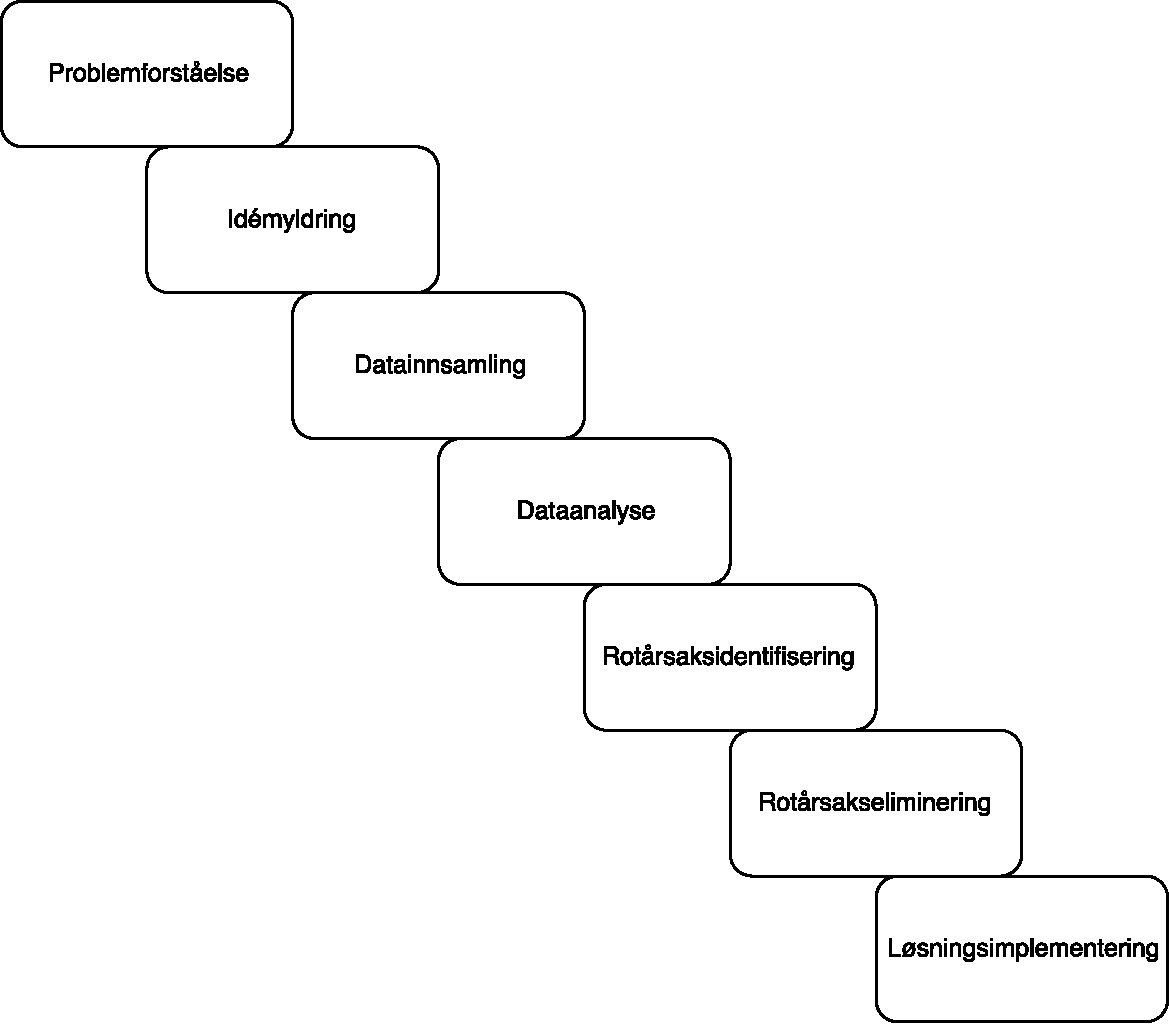
\includegraphics[scale=0.6]{prosess}
    \caption[RCA-prosess]{De syv fasene i rotårsaksanalyseprosessen}
    \label{fig:prosess}
\end{figure}

\subsection{Problemforståelse}
Problemforståelse går ut på å få en solid forståelse for problemet en ønsker å løse og kan også hjelpe med å skape enighet rundt hva problemet egentlig omfatter. Det er også viktig for å passe på at ressursene som benyttes i analysen brukes effektivt videre. Under beskrives de verktøyene som ble brukt av oss i denne fasen. 

\subsubsection{Flytdiagram}
Et flytdiagram viser flyten av aktiviteter i en prosess. I informasjonssikkerhet kan det brukes som en metode for å konkretisere og illustrere et problem ved eller angrep mot virksomhetens aktiva. Formålet er å skape en detaljert forståelse for en prosess som har noe med problemet å gjøre \cite{RCA}.

\subsubsection{Kritiske hendelser}
Hovedpoenget med kritiske hendelser er å identifisere de mest kritiske symptomene i problemet. Det kan hjelpe med å forstå hvilke aspekter ved problemet som trenger å løses, samt forstå problemets natur og konsekvenser for virksomheten \cite{RCA}. Innen informasjonssikkerhet har man ofte logger med hendelsesdata. Det gjør det naturlig å bruke kritiske hendelser siden informasjonen ofte eksisterer på forhånd og trenger bare å bearbeides. 

\subsubsection{Ytelsesmatrise}
Ytelsesmatrise er et diagram som tar i betraktning viktigheten og den nåværende ytelsen til en variabel. Dette gjør at man enkelt kan vurdere hvilken prioritering variablene som blir analysert har \cite{RCA}. Matrisen går fra en til ni på hver akse og er delt inn i fire like store hjørneområder. Ut i fra hvor høy ytelse ytelse og hvor viktige de er, er variablene enten: uviktig, overdrevent, må forbedres eller ok. I informasjonssikkerhet kan det brukes til å vurdere virksomhetens aktiva opp mot for eksempel eksisterende kontroller.

\subsection{Idémyldring}
Målet med idémyldring er å generere så mange idéer som mulig om et gitt emne. I rotårsaksanalyse er målet stort sett å generere en liste over problemområder som kan forbedres, identifisere mulige konsekvenser, generere en liste over mulige årsaker til problemet og oppmuntre til å tenke på løsninger som kan eliminere problemet. Det finnes i hovedsak to typer idémyldring: strukturert og ustrukturert. I strukturert idémyldring har hver deltaker sin tur til å komme med idéer. Dette fører til lik deltagelse og at ingen dominerer prosessen med egne idéer. I ustrukturert idémyldring kan hvem som helst komme med idéer når som helst. Dette er ofte mer spontant, men kan føre til at en person dominerer prosessen \cite{RCA}. 

\subsubsection{Nominell gruppeteknikk (NGT)}
Nominell gruppeteknikk er en strukturert metode for idémyldring som hjelper med å gå fra mange idéer, til å sitte igjen med de beste. Konseptet går ut på å myldre idéer og skrive dem ned på lapper, for så å anonymt gi idéene poeng fra en til fem. Et tallpoeng kan bare gis én gang. Til slutt blir tallene lagt sammen og du sitter igjen med de beste idéene. 

\subsection{Datainnsamling}
Ustrukturert og tilfeldig problemløsning har en tendens til å bli svært unøyaktig. Strukturert rotårsaksanalyse gir derimot et godt grunnlag for blant annet datainnsamlingen, som er en av de sentrale fasene i prosessen. Under beskrives verktøyene som ble brukt for å samle inn informasjon. 

\subsubsection{Spørreundersøkelser}
Spørreundersøkelser brukes når en er på utkikk etter å samle inn data om personers holdninger, følelser eller meninger om et spesifikt problem. En kan skille mellom to typer spørreundersøkelser: kvalitative og kvantitative spørreundersøkelser. Kvantitative undersøkelser handler om å få mange svar slik at en kan ta avgjørelser basert på tall som kan brukes til statistisk analyse. Kvalitative undersøkelser går ut på å samle detaljert informasjon om emnet. Dette kan hjelpe med blant annet å formulere hypoteser for å dirigere kvantitativ undersøkelse senere, eller å komplimentere en kvantitativ undersøkelse ved å bruke sitater fra åpne spørsmål \cite{KvalKvant}. Det brukes ofte elementer fra begge typene når en spørreundersøkelse lages. Når det er snakk om informasjonssikkerhet kan kvalitative undersøkelser brukes når det for eksempel skal samles inn informasjon om brukervaner på nett, eller grad av kunnskap og erfaring om informasjonssikkerhet. Kvalitative undersøkelser kan brukes når det kreves detaljert informasjon om et system eller indre forretningsprosesser. 

\subsubsection{Sampling}
Hovedpoenget med sampling er å trekke ut deler av en populasjon, for å trekke konklusjoner om denne uten å trenge å undersøke alle enhetene \cite{wiki:sample}. I rotårsaksanalyse kan det brukes for å effektivt samle inn data om problemer eller årsaker, og skaffe en bedre forståelse av situasjonen \cite{RCA}.

\subsection{Dataanalyse}
I denne fasen blir dataene analysert og visualisert. Hovedmålet er å avklare mulige rotårsaker som har innvirkning på problemet, og hvilke av de som har størst innflytelse. Under beskrives de ulike verktøyene som ble brukt for å analysere dataene.

\subsubsection{Histogram}
Histogrammer, også kjent som søylediagram, brukes for å vise distribusjon og varians i et datasett. Dataene kan vises i form av lengde, tid, kostnad, mengde osv. Hovedoppgaven til et histogram er å presentere data på en oversiktlig måte slik at det er lett å se mulige relasjoner. I rotårsaksanalyse brukes det til å se hvilke årsaker som dominerer og for å forstå distribusjonen av forskjellige problemer, årsaker, konsekvenser osv. \cite{RCA} Det er viktig å ha minst 30 svar for å lage et gyldig histogram \cite{RCA}.

\subsubsection{Affinitetsdiagram}
Affinitetsdiagram er et verktøy som kan brukes til å analysere kvantitative data. Formålet er å gruppere svar for å finne underliggende relasjoner mellom de resterende gruppene \cite{RCA}. I vår rotårsaksanalyse ble det brukt til å utforske relasjoner mellom forskjellige årsaker, og gruppere relaterte årsaker inn i klasser som kan analyseres kollektivt senere. 

\subsubsection{One-way ANOVA}
ANOVA, også kjent som variansanalyse, er en samlebetegnelse på en rekke statistiske metoder som tester likhet mellom to eller flere utvalg, der én eller flere faktorer gjør seg gjeldene \cite{ANOVA}. 

\subsubsection{Independent-samples t-test}
Dette er en type t-test som brukes for å teste gjennomsnittet mellom to uavhengige grupper på samme avhengige variabel \cite{t-test}. 

\subsection{Rotårsaksidentifisering}
De foregående fasene skal ha generert en liste over mulige rotårsaker og målet i denne er å identifisere de faktiske årsakene. Det kan kreves flere iterasjoner for å finne rotårsaken(e). Verktøy som ble brukt til identifisering er beskrevet under. 

\subsubsection{Årsak-virkningsdiagram (Fiskebeindiagram)}
Et typisk årsak-virkningsdiagram undersøker og analyserer relasjonen mellom et problem og dets årsaker. Det fungerer som en kombinasjon av idémyldring og systematisk analyse. Det brukes for å generere og gruppere årsaker, og evaluere årsakene til problemet for å finne ut hvilke som mest sannsynlig er rotårsaker. Det finnes to typer årsaks-virkningsdiagrammer: fiskebeindiagram og prosessdiagram. Et prosessdiagram er egentlig en samling av fiskebeindiagrammer der hver prosess har sitt eget diagram. Det finnes to ulike tilnærminger til å skape et fiskebeindiagram: spredningsanalyse og årsaksopplisting. Kort forklart, spredningsanalyse grupperer først og idémyldrer etterpå, mens årsaksopplisting idémyldrer først og grupperer etterpå \cite{RCA}. 

\subsubsection{5 Whys}
5 Whys brukes for å undersøke høyere nivåer av årsaker. Som navnet beskriver, går det ut på å spørre ``Why?'' til en bestemt årsak for å komme frem til en ny årsak. Deretter blir det stilt spørsmål til den nye årsaken. Dette gjentar seg helt til det ikke er noen relevante årsaker å komme med. Den siste er da rotårsaken. Som en tommelfingerregel itererer man gjerne fem ganger, men det kan være både flere og færre avhengig av tilfellet. 

\subsubsection{Feiltreanalyse}
Feiltreanalyse er en top-down, deduktiv analyse der en uønsket tilstand av et system analyseres ved hjelp av boolsk logikk for å kombinere en rekke hendelser \cite{wiki:faulttree}. I RCA brukes det for å få en klar oversikt over mulige årsaker, og for å se relasjoner mellom årsaker eller identifisere grupper med relaterte årsaker \cite{RCA}. 

\subsection{Problemeliminering}
Denne fasen innebærer å komme med mulige løsninger til problemet for å eliminere rotårsaken. Boken til Fagerhaug og Andersen \cite{RCA} beskriver to mulige tilnærminger til denne fasen. En tilnærming for å stimulere kreativitet når man leter etter løsninger, og en for å konstruere og utvikle løsninger. Vi har prøvd et verktøy fra hver tilnærming og de er beskrevet under. 

\subsubsection{De seks tenkehattene}
Formålet med de seks tenkehattene er å oppmuntre til å se problemet og løsningene fra forskjellige synsvinkler. Konseptet går ut på at personene får hver sin hatt som skal illustrere deres holdning til problemene \cite{RCA}. 

\begin{description}
    \item[Hvit hatt] skal være kald, nøytral og objektiv, personen skal fokusere på fakta.
    \item[Rød hatt] skal representere sinne, og skal bare fokusere på magefølelsen og egne følelser.
    \item[Svart hatt] skal være pessimistisk og negativ, og fokusere på hvorfor idéen er dårlig.
    \item[Gul hatt] er optimistisk og positiv, og skal fokusere på hvorfor idéen er bra og vil fungere.
    \item[Grønn hatt] representerer gresset, fruktbarhet og vekst, og skal fokusere på å vøre kreativ og komme på nye idéer.
    \item[Blå hatt] er koblet til himmelen, og skal fokusere på å se tingene fra et høyere perspektiv.
\end{description}

\subsubsection{Systematisk Innovativ Tenkning (SIT)}
SIT er en problemelimineringsmetode som baserer seg på konseptet om en ``lukket verden''. Dette betyr at den fokuserer på at løsningene på problemet ofte finnes i det fagområdet problemet eksisterer i. SIT baserer seg på å undersøke en eller flere kjernekomponenter ved hjelp av fem hovedprinsipper \cite{RCA}: 

\begin{description}
    \item[Attributtavhengighet] vurderer å endre en nøkkelvariabel i et produkt for å skape forbedring.
    \item[Komponentkontroll] ser på hvordan et produkt er knyttet til omgivelsene.
    \item[Erstatning] handler om å erstatte en del av et produkt med noe annet fra produktets omgivelser.
    \item[Forkastning] vurderer å forbedre problemet ved å fjerne en komponent. 
    \item[Oppdeling] har som mål å splitte et produkts attributter i to, som for eksempel splittelsen av sjampo fra balsam.
\end{description}

Hovedprinsippet i vårt prosjekt er å fokusere på at løsningene er tilknyttet fagområdet informasjonssikkerhet.

\subsection{Løsningsimplementering}
I den siste fasen er målet å implementere løsningene som ble funnet i foregående fase. I vår rapport vil implementeringen beskrives til beste evne, men ikke implementeres siden vi ikke har mulighet til dette. Implementeringen inkluderer blant annet organisering, utvikling av en implementeringsplan, skape et konsensus om de nødvendige endringene og selvfølgelig implementeringen. Implementeringen av løsningen kan sies å være en suksess når symptomene forsvinner. Verktøyene beskrives under.

\subsubsection{Trediagram}
Et trediagram er et verktøy som er enkelt å bruke og er passende for å dele opp større oppgaver inn i mindre, mer håndterlige aktiviteter. Det er et verktøy som hjelper til å organisere arbeidet som må gjennomføres for å implementere tiltakene som er anbefalt. I informasjonssikkerhet kan dette benyttes for å strukturere oppgavene og planlegge implementeringsprosessen av løsningen. Et trediagram visualiserer hierarkiet i aktivitetene som må gjennomføres, eller enklere sagt, rekkefølgen av gjøremål for å fullføre implementeringen. 

\subsubsection{Kraftfeltsanalyse}
En kraftfeltsanalyse er basert på den oppfatningen at alle situasjoner er resultatet av krefter som virker for og i mot den faktiske tilstanden. En forandring i disse kreftene vil fremkalle en endring, noe som kan brukes til å endre ting i ønsket retning. I rotårsaksanalyse brukes det for å få innsikt i endringsklimaet til en mulig implementering, samt å planlegge aktiviteter som skal til for å implementere løsningen \cite{RCA}. Verktøyet kartlegger krefter som virker for endringen, og krefter som virker i mot. 
\chapter{Gjennomføring av metode}
Dette kapittelet vil gå gjennom bruk av metoden i de tre casene. Det beskrives hvilke verktøy som ble brukt i hver fase, hvorfor vi valgte de, ønsket utbytte av verktøyene, spesifiseringer vi la til grunn og hvordan det ble gjennomført. Tabell \ref{tab:verktoymatrise} under viser de ulike verktøyene vi benyttet i hver fase, i hvert case. 
% Table generated by Excel2LaTeX from sheet 'Ark1'
\begin{table}[htbp]
  \centering
    \caption[Matrise som viser valg av verktøy]{Matrise som viser valg av verktøy fra metoden i de tre casene}
    \begin{tabular}{|l|l|c|r|r|r|}
    \hline
         \cellcolor{yellow} & \cellcolor{yellow} Verktøy & \cellcolor{yellow} Brukt & \multicolumn{1}{c|}{\cellcolor{yellow} Case 1} & \multicolumn{1}{c|}{\cellcolor{yellow} Case 2} & \multicolumn{1}{c|}{\cellcolor{yellow} Case 3} \\
    \hline
    \multicolumn{1}{|l|}{\multirow{4}[8]{*}{Problemforståelse}} & Flytdiagram & x     & \multicolumn{1}{c|}{x} &       &  \\
\cline{2-6}          & Kritiske hendelser & x     & \multicolumn{1}{c|}{x} & \multicolumn{1}{c|}{x} &  \\
\cline{2-6}          & Spiderdiagram & -     &       &       &  \\
\cline{2-6}          & Ytelsesmatrise & x     &       &       & \multicolumn{1}{c|}{x} \\
    \hline
    \multicolumn{1}{|l|}{\multirow{5}[10]{*}{Idémyldring}} & Idémyldring & x     & \multicolumn{1}{c|}{x} & \multicolumn{1}{c|}{x} & \multicolumn{1}{c|}{x} \\
\cline{2-6}          & Idéskriving & -     &       &       &  \\
\cline{2-6}          & Is-is not matrise & -     &       &       &  \\
\cline{2-6}          & NGT   & x     &       &       & \multicolumn{1}{c|}{x} \\
\cline{2-6}          & Parvis sammenligning & -     &       &       &  \\
    \hline
    \multicolumn{1}{|l|}{\multirow{3}[6]{*}{Datainnsamling}} & Sampling & x     &    &  \multicolumn{1}{c|}{x}     &  \\
\cline{2-6}          & Spørreundersøkelse & x     & \multicolumn{1}{c|}{x} & \multicolumn{1}{c|}{x} & \multicolumn{1}{c|}{x} \\
\cline{2-6}          & Sjekkliste & -     &       &       &  \\
    \hline
    \multicolumn{1}{|l|}{\multirow{6}[12]{*}{Dataanalyse}} & Histogram & x     & \multicolumn{1}{c|}{x} & \multicolumn{1}{c|}{x} &  \\
\cline{2-6}          & Paretodiagram & -    &       &        &  \\
\cline{2-6}          & Spredningsdiagram & -     &       &       &  \\
\cline{2-6}          & Problemkonsentrasjonsdiagram & -     &       &       &  \\
\cline{2-6}          & Relasjonsdiagram & -    &       &        &  \\
\cline{2-6}          & Affinitetsdiagram & x     & \multicolumn{1}{c|}{x} & \multicolumn{1}{c|}{x} & \multicolumn{1}{c|}{x} \\
    \hline
    \multicolumn{1}{|l|}{\multirow{4}[8]{*}{Rotårsaksidentifisering}} & Årsak-virkningsdiagram & x     & \multicolumn{1}{c|}{x} & \multicolumn{1}{c|}{x} &  \\
\cline{2-6}          & Matrisediagram & -     &       &       &  \\
\cline{2-6}          & 5 Whys & x     &       & \multicolumn{1}{c|}{x} & \multicolumn{1}{c|}{x} \\
\cline{2-6}          & Feiltreanalyse & x     &       &       & \multicolumn{1}{c|}{x} \\
    \hline
    \multicolumn{1}{|l|}{\multirow{3}[6]{*}{Rotårsakseliminering}} & De seks tenkehattene & x     & \multicolumn{1}{c|}{x} &     &  \\
\cline{2-6}          & TRIZ  & -     &       &       &  \\
\cline{2-6}          & SIT   & x     & \multicolumn{1}{c|}{x} & \multicolumn{1}{c|}{x} & \multicolumn{1}{c|}{x} \\
    \hline
    \multicolumn{1}{|l|}{\multirow{2}[4]{*}{Løsningsimplementering}} & Trediagram & x     & \multicolumn{1}{c|}{x} & \multicolumn{1}{c|}{x} &  \\
\cline{2-6}          & Kraftfeltanalyse & x     &       &       & \multicolumn{1}{c|}{x} \\
    \hline
    \end{tabular}%
  \label{tab:verktoymatrise}%
\end{table}%

Vi kan se over at det er noen verktøy vi har brukt alle casene, og noen vi ikke har brukt i det hele tatt. Under spesifiserer vi grunner til hvorfor dette er tilfellet.

Grunner til bruk av verktøy i alle caser:
\begin{description}
    \item[Idémyldring] ble brukt i alle casene fordi ingen i gruppen dominerte prosessen.
    \item[Spørreundersøkelse] ble brukt i alle casene fordi det var det mest logiske datainnsamlingsverktøyet for hvert av casene.
    \item[Affinitetsdiagram] ble brukt i alle casene fordi vi hadde minst ett spørsmål som var kvalitativt, og det var et behov for å analysere disse.
    \item[SIT] er en utvikling av TRIZ, der TRIZ er mer praktisk rettet. Dette passer ikke alltid så bra i informasjonssikkerhet, og SIT ble heller brukt fordi den er mer friflytene. 
\end{description}

Grunner til at noen verktøy ikke ble brukt i noen av casene:
\begin{description}
    \item[Spiderdiagram] ble ikke brukt fordi det ikke var nødvendig eller mulig med ekstern sammenligning i noen av casene.
    \item[Idéskriving] ble ikke brukt fordi ingen dominerte prosessen, og siden det ikke var behov for å skjule idéer mens de utvikles, ble ikke idéskriving brukt.
    \item[Is-is not matrise] ble ikke brukt fordi forskjeller ikke var forventet.
    \item[Sjekkliste] ble ikke brukt på grunn av tiden det ville ta for å logge hendelser i de ulike casene. 
    \item[Paretodiagram] ble ikke brukt fordi vi ikke hadde tilstrekkelig data til å analysere hvilke årsaker som utgjorde mest effekt. 
    \item[Spredningsdiagram] ble ikke brukt i casene fordi vi ikke hadde noe datasett der resultatene var såpass spredt at spedningsdiagram gir oss noe relevante resultater. 
    \item[Problemkonsentrasjonsdiagram] er i hovedsak fokusert på fysiske lokasjoner, med et fysisk problem. Siden våre caser handler om informasjonssikkerhet, ble det ikke relevant å utføre denne i noen av casene. 
    \item[Relasjonsdiagram] ble ikke brukt fordi vi hadde ikke så altfor mye data i numerisk form. 
    \item[Matrisediagram] ble ikke brukt fordi de andre verktøyene i denne fasen ble ansett som mer passende til det vi ønsket å gjøre.
    \item[TRIZ] er mer praktisk rettet enn SIT, derfor valgte vi heller SIT. 
\end{description}

Verktøyvalgene er i stor grad basert på flytdiagrammene i boka som beskriver vårt utgangspunkt til rotårsaksanalyse \cite{RCA}, og blir valgt basert på disse og et par andre variabler. Flytdiagrammene vi tar utgangspunkt i for hver fase kan sees i vedlegg \ref{flytdiagrammer-verktoyvalg}. I neste avsnitt vil vi gå gjennom alle casene og begrunne verktøyvalg, beskrive ønsket utbytte av verktøyene og dokumentere hvordan de ble brukt, med fokus på spesifiseringen vi la til grunn ved bruk av de. 

%------------------------CASE 1-----------------------------------------
\section{Case 1: Ulovlig fildeling på universitetsnettet}

\subsection{Problemforståelse}

\subsubsection{Flytdiagram}

\paragraph{Valg og ønsket utbytte av verktøy}
Ved å bruke et flytdiagram prøver vi å kartlegge hendelsesforløpet, og hvordan bruksmønsteret til en bruker av nettet til NTNU kan se ut, med fokus på fildeling. Vi håper dette kan gi oss en helhetlig forståelse av hva årsaken til fildeling kan være, og kanskje vi kan bruke dette til å utvikle tiltak senere i prosessen. 

\paragraph{Spesifiseringer}
Det gjøres en antagelse at private fildelingstjenester ikke er med i statistikken fra universitet og at det ikke kommer noen opphavsrettsnotiser fra brukere som bruker private tjenester. Med private tjenester mener vi lukkede nettsamfunn som bare er til for å distribuere opphavsrettsbeskyttet materiale gratis.

\paragraph{Gjennomføring}
Vi fulgte metoden for å lage et flytdiagram, fra boken om rotårsaksanalyse \cite{RCA}.

\begin{enumerate}
    \item Vi samlet alle på gruppen for å diskutere prosessen, og hadde med oss post-it lapper
    \item Vi definerte brukerne som studenter ved NTNU i Gjøvik som bor i Sit Bolig.
    \item Vi definerte hvilke aktiviteter som gjøres for at universitetet skal få en notifikasjon.
    \item Så flyttet vi rundt på lappene til de kom i en naturlig rekkefølge.
\end{enumerate}

\subsubsection{Kritiske hendelser}

\paragraph{Valg og ønsket utbytte av verktøy}
For å gå dypere i detalj har vi tatt en titt på kritiske hendelser som inngår i problemstillingen. Vi har valgt å bruke kritiske hendelser til å dele opp problemet i mindre stykker for å spørre studenter som bor i Sit Bolig om hva de laster ned hvis de først gjør det. Ved bruk av dette verktøyet ønsker vi å få en dypere forståelse av hva studentene laster ned slik at vi kan se om det er noen kategorier som er mest fremtredende. Dette kan føre til at vi blir mer effektive i senere arbeid da vi kan fokusere på det som er viktigst.

\paragraph{Spesifiseringer}
Det er bare studenter som bor i Sit bolig som har blitt registrert som svar. Vi prøvde å være så upartiske som mulig når det kom til valg av respondenter, men det var fortsatt stor overvekt av informatikkstudenter.

\paragraph{Gjennomføring}
Det første som ble gjort var å definere de mest relevante kategoriene av nedlastningsmateriale. Dette ble basert på egen erfaring med blant annet hyppigheten til de ulike kategoriene. Vi hadde en viss anelse om hvilke som var de store synderne, men ønsket å bekrefte våre mistanker. Følgende kategorier ble fremhevet: 
\begin{itemize}
    \item Filmer og serier
    \item Skolebøker
    \item Programvare til skolebruk
    \item Programvare og bøker utenom skolebruk
    \item Spill
    \item Musikk
    \item Annet
\end{itemize}

Intervjuene var i stor grad uformelle ``intervjuer'' med få spørsmål. Det viktigste vi trengte å vite var om personen bodde i Sit Bolig, siden det er bare beboere derfra som er relevante i vår problemstilling, i tillegg til hvilke kategorier de laster ned fra. Resultatene ble fortløpende ført inn i statistikken. Intervjuobjektene var i stor grad bekjente vi visste bodde i Sit Bolig, og derfor var det en overvekt av IT studenter.

Spørsmål stilt til intervjuobjekter:
\begin{itemize}
    \item Bor du, eller har du bodd i Sit Bolig i løpet av studiet? (Hvis nei, avslutt intervju)
    \item Bruker du, eller har du brukt Torrents til å laste ned opphavsrettsbeskyttet materiale mens du bodde i Sit Bolig? Hvis ja, hvilke av følgende kategorier laster du ned fra? (Viser kategoriene)
\end{itemize}


\subsection{Idémyldring}

\paragraph{Valg og ønsket utbytte av verktøy}
Det finnes som sagt flere måter å utføre en idémyldring på, men vi benyttet oss av den ustrukturerte idémyldringen på bakgrunn av verktøyets egenskap til å generere mange idéer hurtig, og på grunn av dens spontane natur. 

\paragraph{Spesifiseringer}
Det er spesielt viktig å ikke omformulere eller diskutere forslagene etterhvert som de kommer, dette skal gjøres etter idémyldringsøkten er over. Vi valgte å strukturere idémyldringen som et tankekart ettersom dette var en kjent løsning for gruppen. 

\paragraph{Gjennomføring}
Det første som ble gjort når økten startet var å kommunisere og skrive opp problemstillingen på en tavle. 

Problemet ble definert som hvorfor personer bruker Torrents til å laste ned opphavsrettsbeskyttet materiale. Når idéstrømmen begynte å gå langsomt, stoppet vi og vurderte det vi hadde kommet fram til. Vi kom blant annet fram til at vi burde spesifisere problemstillingen ytterligere og valgte derfor å spesifisere den til hvorfor folk laster ned på skolenettet. Vi forkortet dette til: ``Hvorfor Torrenting på skolenettet?'' for enkelthets skyld. Det ble kjørt enda en økt med denne nye problemstillingen og vi fikk mer spesifikke resultater.


\subsection{Datainnsamling}

\subsubsection{Spørreundersøkelse}

\paragraph{Valg og ønsket utbytte av verktøy}
I vår situasjon har vi valgt kvantitativ undersøkelse på bakgrunn av et par faktorer. For det første ønsker vi at undersøkelsen skal være helt anonym, siden spørsmålene omhandler potensielle lovbrudd. For det andre er målgruppen et stort antall personer, så det kan være nyttig å samle inn data fra så mange av de som mulig. 

Det vi ønsker å få ut av spørreundersøkelsen er data på utvalgte spørsmål vi mener er relevante for oppgaven. Spørsmålene er utarbeidet for å utforske hvorfor studenter som bor i studentbyer laster ned opphavsrettsbeskyttet materiale, som blant annet inkluderer undersøkelse av økonomiske perspektiver og tilgjengelighet på tjenester. I tillegg ønsker vi også innsikt i hvordan dette kan stoppes.

\paragraph{Spesifiseringer}
Vi brukte Google Forms til å lage spørreundersøkelsen og motta data fra den. Vi setter krav til antall respondenter og utfører en rekke tiltak for å oppnå nok besvarelser, slik at undersøkelsen kan si noe om rotårsaken med relativt høy sikkerhet. Det er et krav å få minst 30 besvarelser som hadde lastet ned opphavsrettsbeskyttet materiale mens de har bodd i hybelen. Videre er det også ønskelig med relativ likhet i antall respondenter mellom de ulike fakultetene og studentbyene. Det hadde vært ideelt med minst 30 respondenter i hver kategori her også, men det er ønsketenkning i denne sammenhengen. Under prosessen ble også totalt antall beboere fra alle studentbyene i Sit Bolig kartlagt. Boligtorget ga oss innbyggertallene fra hver studentby, og vi regnet oss frem til totalt 522 beboere. Det er viktig å presisere at det kan være usikkerheter knyttet til disse tallene, siden det kan hende ikke alle boligene har en beboer.

\paragraph{Gjennomføring}
Hypotesen vi hadde når vi utformet undersøkelsen var at folk laster ned opphavsrettsbeskyttet materiale fordi det er lett tilgjengelig, tilknyttet liten til ingen kostnad og ikke minst fordi det er svært lav risiko for represalier.

En god undersøkelse vil alltid kreve kartlegging av demografi, og i vår undersøkelse valgte vi å kartlegge studentby, kjønn, alder og fakultet. Kjønn og alder er ganske selvforklarende, mens studentby ble valgt på bakgrunn av at Kallerud har mye raskere nedlasting- og opplastingshastighet enn de andre stedene. Vi anså også at det ville være forskjell på hvor mange som laster ned mellom for eksempel informatikkstudiene og helsestudiene. Videre ble resultatene i de foregående fasene brukt til å utforme spørsmålene. Spørreundersøkelsen inkluderer spørsmål om hvor godt en rekke påstander stemmer for den enkelte der respondentene svarer på en likert-skala fra 1-5, der 1 er i liten grad og 5 er i stor grad. Likert-skala ble valgt fordi det er en anerkjent måte å få inn kvantitative svar på hvor enige personer er med en påstand. Samtidig kan man enkelt sammeligne forholdene mellom svarene på de forskjellige påstandene ved hjelp av statistisk analyse. Til slutt inkluderer spørreundersøkelsen et spesielt viktig spørsmål om hva som skal til for at personen stopper med ulovlig nedlasting. Dette er et frisvar der vi kommer til å analysere individuelle svar hver for seg. Spørreundersøkelsen kan leses i sin helhet i vedlegg \ref{undersokelse}.
\newline

Siden spørreundersøkelsen er elektronisk var et av de første tiltakene som ble forsøkt å få tak i en e-post liste fra Sit. Dette fikk vi ikke fra dem. Istedenfor spredde vi den på relevante facebook-sider. Et av prosjektgruppens medlemmer jobber på Studenthuset her på Gjøvik, og fikk spørreundersøkelsen delt på deres facebook-side. Senere i prosessen ble også undersøkelsen delt på facebook-siden til linjeforeningen INGa og klassesidene til sykepleierne og webutvikling. Undersøkelsen ble også delt gjennom venner og bekjente; disse var for det meste informatikkstudenter. I tillegg ble det laget en plakat som ble hengt opp på oppslagstavler på skolen, i vaskeriene ved de ulike studentbyene, og mange ble også plassert i postkassene til Sit sine boliger. Plakaten finnes i vedlegg \ref{plakat}.


\subsection{Dataanalyse}

\subsubsection{Histogram}

\paragraph{Valg og ønsket utbytte av verktøy}
Hovedgrunnen til å bruke histogrammer er for å skape en visuell forståelse av dataene som en ellers ikke får fra tabeller o.l. Da blir det enklere å se korrelasjoner og sammenhenger i datasettet. For dette caset ønsker vi å visualisere hvilke mulige rotårsaker som er mest utbredt, og forstå distribusjonen av hendelser, problemer, årsaker, konsekvenser osv. Analyse av spørsmålene tilknyttet likert-skala er viktig for å finne mulige rotårsaker. Ellers ønsker vi også å finne sammenhenger mellom de ulike spørsmålene, for å se relevante korrelasjoner mellom de.

\paragraph{Spesifiseringer}
Det statistiske verktøyet SPSS ble brukt til å lage histogrammene. For at et histogram skal være gyldig, det vil si hvis vi skal kunne konkludere sikkert med noe, må det være minst 30 svar. 

\paragraph{Gjennomføring}
For å starte analysen eksporterte vi dataene til det statistiske verktøyet SPSS. Deretter ble diagramverktøyene brukt til å lage histogrammer ut fra svarvariablene. Noen spørsmål ble klynget sammen for å kunne se relasjoner mellom variablene visuelt. Vi testet først ut hypotesene våre, deretter ble det sjekket relativt tilfeldig om det var noen andre relevante data å vise i histogrammene. 


\subsubsection{Affinitetsdiagram}

\paragraph{Valg og ønsket utbytte av verktøy}
I spørreundersøkelsen inkluderte vi et kortsvar spørsmål som skulle gi oss svar på hva som kreves for at de stopper med ulovlig fildeling. For å analysere denne dataen var det bare affinitetsdiagram som passet dette. 

\paragraph{Spesifiseringer}
Det nettbaserte verktøyet draw.io ble brukt til å konstruere affinitetsdiagrammet. 

\paragraph{Gjennomføring}
Alle tekstsvarene, inkludert de engelske, ble analysert og kategorisert. Deretter ble dette lagt inn i verktøyet Draw.io og tildelt fargekoder og tallverdier som tilsier hvor mange som svarte i den kategorien. 


\subsubsection{Statistiske analyseverktøy}

\paragraph{Valg og ønsket utbytte av verktøy}
På enkelte spørsmål ble det spurt om påstander og respondentene ble bedt om å svare på en likertskala fra 1-5. Disse dataene er perfekt for å gjøre beregninger på. Derfor har vi valgt å benytte oss av one-way ANOVA analyse og Independent Sample t-test. Vi ønsket å benytte en independent t-test for å undersøke forskjeller mellom variabler der den uavhengige variabelen bestod av to grupper. Vi ville utforske om det var noen signifikant forskjell når det kom til om folk laster ned, mellom Kallerud og de andre studentbyene. I tillegg ville vi se på om det var noen signifikante forskjeller mellom IT fakultetet og de andre fakultetene. Ønsket utbytte ved bruk av ANOVA-analysen er å gi oss et bilde av om påstandene har noen signifikant verdi knyttet til demografien.

\paragraph{Spesifiseringer}
Vi benytter t-test når den uavhengige variablen har to kategorier. One-way ANOVA brukes når det er flere enn to kategorier. Generelt regner vi med en signifikans på: \[\alpha \le 0,05\]

\paragraph{Gjennomføring}
Vi delte opp demografien og ga svarene et tall istedenfor en streng. Vi delte inn Kallerud og de andre studentbyene hver for seg, siden det var få svar på de andre studentbyene, slik at det ble jevn fordeling. Det samme ble også gjort med IT og de andre fakultetene. 

Forholdet mellom tallverdiene og svarkategoriene er som følger:

Kjønn:
\begin{itemize}
    \item Kvinne: 1
    \item Mann: 2
\end{itemize}

Fakultet:
\begin{itemize}
    \item Fakultet for arkitektur og design: 1
    \item Fakultet for informasjonsteknologi og elektroteknikk: 2
    \item Fakultet for ingeniørvitenskap: 3
    \item Fakultet for medisin og helsevitenskap: 4
    \item Fakultet for økonomi: 5
\end{itemize}

Når det er bare snakk om IT fakultetet mot andre:
\begin{itemize}
    \item Andre fakulteter: 1
    \item Fakultet for informasjonsteknologi og elektroteknikk: 2
\end{itemize}

Alder:
\begin{itemize}
    \item Under 20: 1
    \item 20-25: 2
    \item 26-30: 3
    \item 31-35: 4
    \item Over 35: 5
\end{itemize}

Studentby (Kallerud mot andre):
\begin{itemize}
    \item Kallerud: 1
    \item Andre studentbyer: 2
\end{itemize}

Har du lastet ned:
\begin{itemize}
    \item Nei: 1
    \item Ja: 2
\end{itemize}


\subsection{Rotårsaksidentifisering}


\subsubsection{Årsak-virkningsdiagram}

\paragraph{Valg og ønsket utbytte av verktøy}
I dette caset var det kommet frem til hovedårsaker som ble relevante til å sette inn i et fiskebeindiagram. Ved bruk av dette verktøyet ønsker vi å sitte igjen med en visuell fremstilling av rotårsaken til problemet. Dette vil gjøres ved å identifisere hva som skaper årsakene som kom frem av dataanalysen. 

\paragraph{Spesifiseringer}
Det er anbefalt å bruke en tusjtavle for å tegne opp fiskebeindiagrammet, men vi valgte å bruke et nettbasert program som er laget for å skape diagrammer med flere brukere involvert i sanntid. De hadde en egen mal for fiskebeindiagram som vi valgte å gå ut fra.

\paragraph{Gjennomføring}
Stegene vi fulgte i prosessen er hentet fra boka om rotårsaksanalyse \cite{RCA} og ble som følger:

\begin{enumerate}
    \item Vi beskrev problemet klart og tydelig
    \item Vi tegnet opp problemet på slutten av fiskebeindiagrammet
    \item Vi identifiserte hovedkategoriene av årsakene til problemet og tegnet det opp på fiskebeinene i diagrammet
    \item Vi idémyldret alle mulige årsaker i hver kategori, en kategori om gangen, og skrev det inn i diagrammet fortløpende
    \item Til slutt analyserte vi de identifiserte årsakene og bestemte de mest sannsynlige rotårsakene
\end{enumerate}


\subsection{Rotårsakseliminering}

\subsubsection{De seks tenkehatter}

\paragraph{Valg og ønsket utbytte av verktøy}
I denne fasen har vi valgt å bruke vektøyet seks tenke hatter fordi vi ville stimulere til kreativitet når forslag ble fremmet. Ønsket utbytte med bruk av seks tenkehatter, er å skape en forståelse rundt rotårsaken og komme opp med mulige tiltak for å eliminere problemet. Siden problemet virker vanskelig å fikse fra universitetet sin side måtte vi komme med noen kreative løsninger, og de seks tenkehattene fungerer godt for dette. 

\paragraph{Spesifiseringer}
Siden vi bare var fire, og det egentlig kreves seks, måtte to av oss innehave to roller samtidig. 

\paragraph{Gjennomføring}
Siden vi bare var fire tok to av oss på seg to hatter og resten en. Så startet vi å diskutere problemstillingen og hvordan vi burde gå inn for å eleminere rotårsaken. Hver enkelt gruppemedlems tilnærming var basert på hatten de hadde på hodet. Etter at vi var ferdig med de seks tenkehattene gikk vi fort igjennom de forskjellige forslagene, for å se på hva som var praktisk gjennomførbart. De andre forslagene ble luket bort. 


\subsubsection{Systematisk Innovativ Tenkning}

\paragraph{Valg og ønsket utbytte av verktøy}
Vi har valgt å benytte SIT i henhold til boken \cite{RCA}. Ønsket utbytte med bruk av seks tenkehatter, er å skape en forståelse rundt rotårsaken og komme opp meg mulige tiltak for å eliminere problemet. Siden problemet virker vanskelig å fikse fra universitetet sin side måtte vi komme med kreative løsninger. De seks tenkehattene fungerer godt til dette.

\paragraph{Spesifiseringer}
Ikke alle hovedprinsippene kunne gi tiltak. Der det ikke var mulig ble det presisert ``Ikke gjennomførbart''. 

\paragraph{Gjennomføring}
Det første som ble gjort var å liste opp alle komponenter som eksisterer i problemets naturlige omgivelser. Deretter ble hver komponent analysert ut fra de fem hovedprinsippene til SIT, der tiltak ble beskrevet. De mest lovende tiltakene ble tatt videre til en mer detaljert gjennomgang. Deretter ble det plukket ut fra de igjen, de tiltak som var mest egnet, og ble videre ført inn i en tiltaksplan. 


\subsection{Løsningsimplementering}

\subsubsection{Trediagram}

\paragraph{Valg og ønsket utbytte av verktøy}
Trediagram benyttes for å skape en liste over aktiviteter som må gjennomføres for å innføre de spesifikke tiltakene. 

\paragraph{Spesifiseringer}
Diagrammverktøyet draw.io ble brukt til å konstruere trediagrammet. 

\paragraph{Gjennomføring}
Dette verktøyet startet med å gruppere hovedtiltak til rotårsaken, deretter ble hver aktivitet som må gjennomføres for at tiltaket skal bli gjennomført gruppert. Disse underpunktene ble gruppert etter hvilken rekkefølge de skal bli implementert slik at tiltaket er mulig å gjennomføre. 


%------------------------CASE 2------------------------------------------
\newpage
\section{Case 2: Kompromitterte brukerkontoer ved NTNU}

\subsection{Problemforståelse}

\subsubsection{Kritiske hendelser}

\paragraph{Valg og ønsket utbytte av verktøy}
For å lære mer om bakgrunnen til problemet bruker vi verktøyet kritiske hendelser for å se på frekvensen av misbruk som er registrert fra de kompromitterte kontoene. Slik kan vi kartlegge og forstå hva de kompromitterte kontoene brukes til. Ved bruk av dette verktøyet ønsker vi å få en oversikt over hvilke handlinger de kompromitterte kontoene utfører. Dette går i stor grad ut på hva som er motivasjonen til trusselaktørene. Vi ønsker å danne et bilde av hva de ønsker å oppnå ved å kompromittere kontoene, slik at vi kan bruke den informasjonen senere til å finne rotårsaken til at de blir kompromittert. 

\paragraph{Spesifiseringer}
Informasjonen som brukes i dette verktøyet ble gitt av oppdragsgiver. Dataene sier bare noe om frekvensen av sikkerhetshendelser, og ikke noe om viktigheten.

\paragraph{Gjennomføring}
Sammen med oppgavebeskrivelsen fikk vi en liste over loggførte sikkerhetshendelser som hadde foregått det siste året hvor kompromitterte kontoer var involvert. Dataene ble sortert i synkende rekkefølge og lagt inn i en tabell for å visualisere frekvensen til de enkelte sikkerhetshendelsene, og dermed fokusområdene til trusselaktørene. 


\subsection{Idémyldring}

\subsubsection{Valg og ønsket utbytte av verktøy}
Vi har valgt å benytte idémyldring på basis av RCA boken \cite{RCA} sin fremgangsmåte for valg av verktøy, og på bakgrunn av vår tidligere kunnskap om hvordan brukere vanligvis kompromitteres. Vi valgte å organisere idémyldringen som et tankekart ettersom dette var en kjent løsning for gruppen. Den ustrukturerte tilnærmingen til idémyldring ble brukt på grunn av dens uformelle struktur. Ingen er heller dominerende i gruppen, som gjør det mulig for alle å komme med innspill. Hvis noen i gruppen hadde vært dominerende hadde vi heller gått over til å bruke skriftlig idémyldring, også kjent som idéskriving. Ønsket utbytte ved å bruke idémyldring var for å få en forståelse av hva som kan være rotårsaken til at ansatte sine kontoer blir kompromittert, og hvordan passord og brukernavn kan komme på avveie. 

\subsubsection{Spesifiseringer}
Det er spesielt viktig å ikke omformulere eller diskutere forslagene etterhvert som de kommer, dette skal gjøres etter idémyldringsøkten er over.

\subsubsection{Gjennomføring}
Det første som ble gjort når økten startet var å kommunisere og skrive opp problemstillingen på en tavle. Vi diskuterte og prøvde å komme på mulige måter trusselaktører kan kompromittere brukerkontoer til de ansatte ved universitetet, og hvordan passord og brukernavn kan komme på avveie.


\subsection{Datainnsamling}

\subsubsection{Spørreundersøkelse}

\paragraph{Valg og ønsket utbytte av verktøy}
Grunnen til at vi valgte i hovedsak kvantitativ spørreundersøkelse er at vi ønsker å finne relasjoner mellom dataene vi samler inn. Det er også mulighet for å gjøre statistiske beregninger på disse, noe vi anser som relevant for datainnsamlingen i dette caset. Fremstilling av data i grafer og tabeller er også et moment som gjorde at valget ble kvantitativ metode. Med den elektroniske spørreundersøkelsen ønsker vi å få informasjon fra personer som allerede har fått brukeren sin kompromittert. Informasjonen vil bestå av blant annet personens passordvaner, kjennskap til retningslinjer om passordbruk og epost-aktivitet. Vi håper å få minst 30 respondenter, som vil være akkurat nok for en kvalitativ analyse. 

\paragraph{Spesifiseringer}
Undersøkelsen var kvalitetskontrollert flere ganger av forskjellige personer, inkludert medstudenter, veileder og ikke minst oppdragsgiver. Undersøkelsen ble laget i SelectSurvey, med tilhørende NTNU tema for utformingen. Dette ble gjort for å få spørreundersøkelsen til å virke legitim, siden den har NTNU sin logo i hjørnet og nettadressen tilhører NTNU sitt domene. Noen av spørsmålene skal besvares på en skala fra 1-6. Denne skalaen valgte vi fordi vi ville tvinge respondentene til å havne på den ene eller andre siden av spekteret, og ikke velge i midten dersom de ikke visste. 

Spørreundersøkelsen ble sendt ut til totalt 167 personer, men den nådde bare 157 av e-post addressene. Alle disse hadde fått sin NTNU konto kompromittert i tidsperioden 1. November 2016 til 1. April 2018. E-post listen ble opprettet av oppdragsgiver basert på intern data og sent ut på vegne av Seksjon for Digital Sikkerhet. 

Det ble oppdaget et par småfeil i spørreundersøkelsen etter den var utsendt. Blant annet var det glemt et ``vet ikke'' alternativ på spørsmålet om de hadde en formening om hvor lang tid det hadde gått fra kompromittering til de fikk beskjed. Dette fikk vi fikset ved å legge til tekst om at du kunne la det være blankt om du ikke visste, slik at det ikke gikk altfor mye ut over svarene, og spørsmålet ble endret til å ikke være obligatorisk. Det var også glemt en kommentarboks helt i slutten av spørreundersøkelsen, som vi bestemte at vi ikke kunne plassere inn etter den var utsendt. Det var også et par småfeil i formulering, men dette fikk vi endret underveis. Endringene ble gjort på natten da vi antok ingen svarte. 

\paragraph{Gjennomføring}
Det første som ble gjort var å finne ut hva vi ville ha informasjon om. Deretter ble spørsmål for å få svar på dette lagd. Videre definerte vi hypoteser til nesten hvert spørsmål. Vi skrev også en tekst som skulle bli sendt ut sammen med spørreundersøkelsen for å oppmuntre til å ta den. Her ble det brukt mye patos ettesom dette er et ømfintlig tema. Undersøkelsen ble sendt ut på fredag 20. April. 


\subsection{Dataanalyse}

\subsubsection{Histogram}

\paragraph{Valg og ønsket utbytte av verktøy}
Vi har igjen valgt å benytte histogrammer for å fremlegge dataene fra spørreundersøkelsen. Dette gjøres fordi det er en god måte å fremstille data på et tilfredstillende vis for leserne. Ved å benytte histogram håper vi å få en visuell fremstilling av data som gjør det raskt og enkelt å forstå disse, og derfor lettere kunne trekke konklusjoner. I dette caset vil histogrammer stort sett bli brukt for å få en oversikt over svarprosent på enkeltsspørsmål. 

\paragraph{Spesifiseringer}
Det statistiske verktøyet SPSS ble brukt til å lage histogrammene. For at et histogram skal være gyldig, det vil si hvis vi skal kunne konkludere sikkert med noe, må det ha minst 30 svar. 

\paragraph{Gjennomføring}
Dataene ble eksportert til SPSS og diagramverktøyet ble valgt for å konstruere histogrammene. Deretter ble de analysert og eksportert til rapporten dersom et resultat ble funnet. 


\subsubsection{Affinitetsdiagram}

\paragraph{Valg og ønsket utbytte av verktøy}
Et av spørsmålene i spørreundersøkelsen var et kortsvar der respondentene kunne svare om de hadde noen formening om hvordan de ble kompromittert. Ved å bruke affinitetsdiagram håper vi på å få samlet og gruppert disse dataene slik at vi kan se om noe blir sagt flere ganger, og kan være en mulig årsak. 

\paragraph{Spesifiseringer}
Det nettbaserte verktøyet draw.io ble brukt til å konstruere affinitetsdiagrammet. 

\paragraph{Gjennomføring}
Hvert enkelt svar ble analysert hver for seg og gruppert under en av mange hovedkategorier. Deretter ble disse hovedkategoriene tegnet som bokser i nettleserverktøyet Draw.io. Disse boksene inkluderer frekvens av svar og differensiering av svarene under hovedkategoriene. 


\subsubsection{Statistiske analyseverktøy}

\paragraph{Valg og ønsket utbytte av verktøy}
Spørreundersøkelsen inkluderer blant annet spørsmål om kjennskap til ulike dokumentasjon og bevissthet på sikkerhet. Dette er spørsmål som blir besvar på en skala fra 1-6. Dette er data som statistisk analyse kan bli benyttet på. Det er også mange ja/nei spørsmål som disse verktøyene kan brukes på. Ved å bruke statistiske analyseverktøy som ANOVA og Independent-samples t-test ønskes det å finne tilsynelatende skjulte relasjoner eller forskjeller mellom demografien og kjennskap til retningslinjer, bevissthet på sikkerhet og e-post og passordvaner. Vi ønsker også å se om det er noen relasjoner mellom andre spørsmål. ANOVA ble brukt dersom den uavhengige variabelen består av mer enn to grupper. Dersom den bestod av to grupper ble Independent t-test heller brukt.

\paragraph{Spesifiseringer}
Vi benytter t-test når den uavhengige variablen har to grupper. One-way ANOVA brukes når det er flere enn to grupper. Generelt regner vi med en signifikans på: \[\alpha \le 0,05\]

\paragraph{Gjennomføring}
For demografien og de andre spørsmålene som ikke hadde tallsvar, ble svarene transformert til tall. 

Forholdet mellom tallverdiene og svarkategoriene er som følger:

Kjønn:
\begin{itemize}
    \item Mann: 1
    \item Kvinne: 2
\end{itemize}

Primærrolle:
\begin{itemize}
    \item Ansatt: 1
    \item Student: 2
\end{itemize}

År ved NTNU:
\begin{itemize}
    \item Under 2: 1
    \item 2-4: 2
    \item 5-9: 3
    \item 10-15: 4
    \item Over 15: 5
\end{itemize}

Alle Ja/Nei spørsmål:
\begin{itemize}
    \item Ja: 1
    \item Nei: 2
\end{itemize}

Deretter ble testene kjørt på variablene. 


\subsection{Rotårsaksidentifisering}

\subsubsection{Årsak-virkningsdiagram}

\paragraph{Valg og ønsket utbytte av verktøy}
I dette caset har vi valgt et fiskebeindiagram på bakgrunn av at årsakene er spredt over flere variabler, og det er mulig at ytterligere årsaker eksisterer. Ved bruk av dette verktøyet ønsker vi å sitte igjen med en visuell fremstilling av rotårsakene til problemet. Dette vil gjøres ved å identifisere hva som skaper årsakene vi har funnet frem til i foregående fase. 

\paragraph{Spesifiseringer}
Det er anbefalt å bruke en tusjtavle for å tegne opp fiskebeindiagrammet, men vi valgte å bruke det nettbaserte programmet draw.io \cite{drawio}. Draw.io er laget for å skape diagrammer med flere brukere involvert i sanntid. De hadde en egen mal for fiskebeindiagram som vi valgte å gå ut fra.

\paragraph{Gjennomføring}
Stegene vi fulgte i prosessen er hentet fra boka om rotårsaksanalyse \cite{RCA} og ble som følger:

\begin{enumerate}
    \item Først ble problemet definert og skrevet i slutten av fiskebeindiagrammet.
    \item Deretter ble hovedkategoriene skrevet ned i bokser. Disse er direkte tilknyttet resultatene fra analysen.
    \item Videre startet vi å idémyldre alle mulige årsaker under hver kategori, en kategori om gangen. Disse ble fortløpende skrevet inn i diagrammet.
    \item Til slutt analyserte vi de identifiserte årsakene og bestemte de mest sannsynlige rotårsakene
\end{enumerate}


\subsubsection{5 Whys}

\paragraph{Valg og ønsket utbytte av verktøy}
Etter fiskebeindiagrammet mente vi at det var sannsynlig at høyere nivå av årsaker kunne eksistere bak de identifiserte årsakene. Ved å bruke 5 Whys er det ønskelig å konfirmere om årsakene som ble fremhevet i fiskebeindiagrammet er faktiske rotårsaker, og ikke bare lav-nivå årsaker. 

\paragraph{Spesifiseringer}
Det ble tatt utgangspunkt i fem iterasjoner, men det er mulighet for flere eller færre avhengig av om spørsmålet kan besvares på en fornuftig måte. 

\paragraph{Gjennomføring}
Med dette verktøyet tar vi utgangspunkt i casebeskrivelsen, nemlig rotårsaken til kompromitterte kontoer ved NTNU. Ut fra dette brukte vi årsaker fra fiskebeindiagrammet over for å komme på årsaker som skal analyseres, samt prøvde å idémyldre et par nye. For hver av disse årsakene ble det spurt: ``Hvorfor er dette en årsak av det orginale problemet?''. For hvert svar spør vi hvorfor igjen og igjen helt til vi finner rotårsaken. 

\subsection{Rotårsakseliminering}

\subsubsection{Systematisk Innovativ Tenkning (SIT)}

\paragraph{Valg og ønsket utbytte av verktøy}
Grunnen til at SIT ble valgt er at vi mener problemet kan løses i problemets naturlige omgivelser. Ved å bruke SIT metoden ønsker vi å få kreative idéer på hvordan vi kan finne en løsning til kompromitterte kontoer ved NTNU. 

\paragraph{Spesifiseringer}
SIT burde helst gjennomføres av 10-12 personer fra en rekke forskjellige fagområder, men siden vi ikke hadde så mange tok vi bare utgangspunkt i prosjektgruppen. Ikke alle SIT-prinsipper finner løsninger som er gjennomførbare for alle komponenter. I disse tilfellene vil det stå: ``Ikke gjennomførbart''. 

\paragraph{Gjennomføring}
Først ble alle komponentene som omhandler problemet listet opp. Etter det ble de fem hovedprinsippene fra SIT brukt sekvensielt på komponentene for å utvikle løsninger på problemene. Deretter ble de mest relevante løsningene valgt ut og beskrevet i ytterligere detalj. Videre ble de mest realistiske og gjennomførbare idéene trukket ut og fremhevet i en tiltaksplan.


\subsection{Løsningsimplementering}

\subsubsection{Trediagram}

\paragraph{Valg og ønsket utbytte av verktøy}
For å få en oversikt over hva som må gjøres for å implementere tiltaksplanen bruker vi Trediagram til å dele opp aktivitetene og bestemme rekkefølgen. Ønsket utbytte ved å bruke trediagram er å redegjøre for og strukturere de aktiviteter som må gjøres for å innføre de spesifikke tiltakene. 

\paragraph{Spesifiseringer}
Trediagrammets aktiviteter gjøres i samme rekkefølge som en postorder trealgoritme. Dette betyr at aktivitetene gjøres fra venstre til høyre, der en starten nederst til venstre. Det er derimot ingen gitt rekkefølge man kan innføre tiltakene i, og noen tiltak vil ikke kunne eller behøve å innføre sammen. 

\paragraph{Gjennomføring}
Gjennomføringen av trediagrammet startet ved å gruppere hovedtiltak til rotårsaken. Deretter ble hver aktivitet som må gjennomføres for at tiltaket skal bli gjennomført delt opp. Disse underpunktene ble plassert etter hvilken rekkefølge de skal bli implementert slik at tiltaket er mulig å gjennomføre. 


%------------------------CASE 3-----------------------------------------
\newpage
\section{Case 3: Misbruk av NTNU sin infrastruktur til utvinning av kryptovaluta}

\subsection{Problemforståelse}
\subsubsection{Ytelsesmatrise}

\paragraph{Valg og ønsket utbytte av verktøy}
Vi har valgt å benytte ytelsesmatrise i dette caset for å utforske bruk av et nytt verktøy. Det ble også valgt fordi det er fordelaktig å undersøke de eksisterende kontrollene og fokusere på de kontrollene som ikke fungerer som ønsket. Ved bruk av dette verktøyet er det ønskelig å undersøke hvordan eksisterende kontroller fungerer i forhold til deres viktighet for NTNU. 

\paragraph{Spesifiseringer}
Vi definerte viktighet som hvor mye IT-reglementet stopper utvinning av kryptovaluta. Ytelse ble satt effekten av de eksisterende kontrollene som er i IT-reglementet per nå.

\paragraph{Gjennomføring}
Prosessen startet ved å finne ut hvilke aspekter av problemet som skulle vurderes. Gruppen kom fram til å vurdere formene for kontroller som stopper eller reduserer sjansen for at trusselaktørene misbruker NTNU sin infrastruktur. 


Disse skulle vurderes basert på viktighet og ytelse. 

Matrisen ble tegnet opp i Excel der hver akse ble konstruert fra en til ni, og matrisen ble delt inn i fire områder:
\begin{description}
    \item[Uviktig:] Når både viktigheten og ytelsen er fra en til fem.
    \item[Overdrevent:] Når viktigheten er fra en til fem og ytelsen er fra fem til ni.
    \item[Ok:] Når både viktigheten og ytelsen er fra fem til ni.
    \item[Må forbedres:] Når viktigheten er fra fem til ni, mens ytelsen bare er fra en til fem.
\end{description}

\subsection{Idémyldring}

\subsubsection{Idémyldring}
\paragraph{Valg og ønsket utbytte av verktøy}
Vi har valgt å benytte Idémyldring på basis av RCA boken \cite{RCA} sin fremgangsmåte for valg av verktøy. 
Vi ønsker ved bruk av idémyldring å få en forståelse av hva som kan være rotårsaken til at NTNU sine ressurser blir misbrukt til utvinning av kryptovaluta. Vi ønsker også å skape et godt grunnlag av idéer som kan brukes i datainnsamling i neste del av oppgaven.

\paragraph{Spesifiseringer}
Det er spesielt viktig å ikke omformulere eller diskutere forslagene etterhvert som de kommer, dette skal gjøres etter idémyldringsøkten er over. Det ble gjennomført to idémyldringer på forskjellige aspekter av problemet. 

\paragraph{Gjennomføring}
Vi startet idémyldringen med å finne ut hva som burde fokuseres på av hvordan og hvorfor skolen sine ressurser blir misbrukt til utvinning av kryptovaluta. Vi kom frem til at begge deler var like viktige, og at vi burde ha to idémyldringer for å komme med flest mulige idéer som ville kunne hjelpe oss i hva som burde spørres om i datainnsamlingen. Den første idémyldringen omhandlet hvordan, mens den andre omhandlet hvorfor NTNU sine ressurser blir misbrukt til utvinning av kryptovaluta. Idémyldring prosessen var litt annerledes enn de vi hadde i de andre oppgavene. Denne gangen lignet det mer på idéskriving, der vi alle skrev inn idéene våre i et dokument. Det kunne fortsatt ikke defineres som det metoden beskriver som idéskriving siden dette ikke var anonymt.


\subsubsection{Nominell gruppeteknikk (NGT)}
\paragraph{Valg og ønsket utbytte av verktøy}
Ettersom vi har dårligere tid på dette caset enn på de tidligere, har vi valgt å benytte NGT for å prioritere idéer. NGT er også et verktøy vi er interessert i å prøve ut for hovedrapporten.

\paragraph{Spesifiseringer}
Ingen.

\paragraph{Gjennomføring}
NGT ble utført ved at alle satte seg ned sammen og hadde 15 poeng hver å gi til forskjellige idéer. Idéene ble laget utifra forarbeidet som var blitt gjort i idémyldringsprosessen. De idéene som lignet på hverandre ble slått sammen og noen ble omformulert. Hver deltaker delte ut 1, 2, 3, 4 eller 5 poeng til idéene de mente var best. Dette var basert på hva de trodde ville være det viktigste å fokusere på videre i analysen. Etter vi var ferdige, gikk oppdragsgiver igjennom resultatene. Disse dataene kan sees i tabell \ref{tab:NGT}.

\subsection{Datainnsamling}
\subsubsection{Intervju}

\paragraph{Valg og ønsket utbytte av verktøy}
Siden vi hadde begrenset med tid (en måned), valgte vi å begrense informasjonsinnsamlingen til ett kvalitativt intervju. 

Ønsket utbytte med dette intervjuet er å få et overblikk over hvordan utvinningsverktøy blir brukt, og hvordan de eksterne aktørene får verktøyene inn på PCene til de som oppholder seg på nettet til NTNU.

\paragraph{Spesifiseringer}
På grunn av tidsbegrensningen og problemets tekniske art, begrenser vi datainnsamlingen til ett intervju.
Det ble tatt lydopptak av intervjuet. Dette ble transkribert i etterkant. 

\paragraph{Gjennomføring}
Intervjuet ble gjennomført med en senior sikkerhetsanalytiker som jobber på SOCen til NTNU. 

Vi utformet et intervju der spørsmålene bestod av diverse temaer vi ønsket å belyse for å finne rotårsaken. En del av spørsmålene gikk ut på å finne ut hvordan utvinningen blir oppdaget, hva slags handlingsrom de har for å håndtere hendelser og hvordan utvinningen som regel foregår.

Under intervjuet spurte vi om vi fikk ta lydopptak, og vi fikk ja til dette. Dermed kunne vi lett gå tilbake til svarene for å få det mest mulig nøyaktig til neste fase. Dette ble transkribert i etterkant. 

\subsection{Dataanalyse}
\subsubsection{Affinitetsdiagram}

\paragraph{Valg og ønsket utbytte av verktøy}
Dataene våre besto ikke av nummere, men meninger og idéer så derfor har vi benyttet affinitetsdiagram.

Ønsket utbytte av å bruke affinitetsdiagram er å finne bindinger eller fellesnevnere som kan være til hjelp for å fjerne rotårsaken.

\paragraph{Spesifiseringer}
Det nettbaserte verktøyet draw.io ble brukt til å konstruere affinitetsdiagrammet.

\paragraph{Gjennomføring}
Analysen ble gjennomført ved å bruke transkripsjon fra intervjuet og stykke svarene opp i fem hovedgrupper. Disse hovedgruppene ble utredet mens analysen ble gjennomført.

\subsection{Rotårsaksidentifisering}
\subsubsection{5 Whys}

\paragraph{Valg og ønsket utbytte av verktøy}
Vi valgte å benytte 5 whys siden vi mener det er sannsynlig at det finnes høy-nivå årsaker. 

Ved å bruke 5 Whys er det ønskelig å finne rotårsaken til årsakene fremhevet i affinitetsdiagrammet. Målet her er å få frem rotårsaker, som vi kan bruke videre i rotårsakselimineringen. 

\paragraph{Spesifiseringer}
Vi tok utgangspunkt i å spørre ``hvorfor'' til vi fant rotårsaker. Om vi følte det vi kom frem til gikk veldig langt fra problemet, skulle vi gå et steg tilbake og prøve igjen; spesielt om vi kommer ned til lønnsomhet. Dette gjør vi fordi lønnsomhet kan være en rotårsak til at folk driver med utvinning, men ikke nødvendigvis til at dette skjer på NTNU. 

\paragraph{Gjennomføring}
Med dette verktøyet tar vi utgangspunkt i casebeskrivelsen; nemlig rotårsaken til kryptoutvinning på NTNU. Ut fra dette brukte vi funnene fra analysen for å komme på årsaker, samt prøvde å idémyldre et par nye. For hver av disse årsakene ble det spurt: ``Hvorfor er dette en årsak av det originale problemet?''. For hvert svar spør vi hvorfor igjen og igjen helt til vi finner rotårsaken. Det ble tatt utgangspunkt i fem iterasjoner, men det er mulighet for flere eller færre avhengig av om spørsmålet kan besvares på en fornuftig måte. 

\subsubsection{Feiltreanalyse}
\paragraph{Valg og ønsket utbytte av verktøy}
Ettersom det var flere årsaker som var bundet sammen etter gjennomføring av 5 Whys, valgte vi å benytte feiltreanalyse.

Ved bruk av dette verktøyet ønsker vi å få en oversikt over relasjoner mellom de forskjellige årsakene. Vi ønsker også å få sortert ut de årsakene som NTNU ikke har mulighet til å gjøre noe med.

\paragraph{Spesifiseringer}
Analysen bygger på hva som ble gjort i 5 Whys. Verktøy som ble brukt til utforming av tabellen var draw.io.

\paragraph{Gjennomføring}
Med dette verktøyet tar vi utgangspunktet i resultatene fra 5 Whys til å finne rotårsakene. Her gikk vi steg for steg nedover og ser på årsaken til at enhver uønsket hendelse inntreffer.


\subsection{Rotårsakseliminering}
\subsubsection{Systematisk Innovativ Tenkning (SIT)}

\paragraph{Valg og ønsket utbytte av verktøy}
Vi ville opprinnelig se på hvordan TRIZ fungerer. Da vi studerte verktøyet nøyere kom vi fram til at det kun var brukt til fysiske produkter. Seks tenkehatter ble ikke gjort da vi kun var to personer på denne delen. SIT ble valgt da vi ikke har vært helt fornøyd med verktøyet i de tidligere casene og vi ønsket å se om det er casene eller verktøyet sin feil.
  

\paragraph{Spesifiseringer}
SIT burde helst gjennomføres av 10-12 personer, fra en rekke forskjellige fagområder, men siden vi ikke hadde så mange tok vi bare utgangspunkt i prosjektgruppen. Ikke alle SIT-prinsipper finner løsninger som er gjennomførbare for alle komponenter. I disse tilfellene vil det stå: ``Ikke gjennomførbart''. 

\paragraph{Gjennomføring}
Det første som ble gjort var å liste opp alle komponenter som eksisterer i problemets naturlige omgivelser. Deretter ble hver komponent analysert ut fra de fem hovedprinsippene til SIT, der tiltak ble beskrevet. De mest lovende tiltakene ble tatt videre til en mer detaljert gjennomgang. Deretter ble det plukket ut fra de igjen, de tiltak som var mest egnet, og ble videre ført inn i en tiltaksplan. 

\subsection{Løsningsimplementering}
\subsubsection{Kraftfeltsanalyse}

\paragraph{Valg og ønsket utbytte av verktøy}
Vi valgte kraftfeltsanalyse fordi vi vi ville teste ut flere verktøy.

Ønsket utbytte fra kraftfeltsanalyse er å få vite hva som er for og hva som er mot implementering av tiltakene. Dette verktøyet gir en oversikt over hvilke tiltak som er lettest å gjennomføre.

\paragraph{Spesifiseringer}
Ingen.

\paragraph{Gjennomføring}
Kraftfeltsanalysen ble gjort ved at vi tok tiltakene fra problemelimineringen og hadde en idémyldring for å se hva som talte for og imot tiltakene. Deretter ble styrken av disse kreftene estimert. Tilslutt ble alt lagt inn i en figur som viser styrkene både for og imot et gitt tiltak. 

\section{Case 1: Ulovlig fildeling på skolenettet}

\chapter{Resultater og analyse fra Case 2: Kompromitterte brukerkontoer ved NTNU}
I dette kapittelet fremlegger vi våre resultater i alle fasene i case 2.

\section{Problemforståelse}

\subsection{Kritiske hendelser}
Sammen med oppgavebeskrivelsen fikk vi en liste over loggførte sikkerhetshendelser som hadde foregått det siste året hvor kompromitterte kontoer var involvert. Dataene ble sortert i synkende rekkefølge og lagt inn i en tabell for å visualisere frekvensen til de enkelte sikkerhetshendelsene, og dermed fokusområdene til trusselaktørene. 

\begin{table} [H]
    \begin{tabular}{ | m{18em} | m{18em} | }
        \hline
            \cellcolor{yellow} Sikkerhetshendelser & \cellcolor{yellow} Frekvens \\
        \hline
            Spam & 46  \\
        \hline
            Misuse (uthenting av forskningsartikler) & 26 \\
        \hline
            Negligible/Fixed/Failed Attack  & 8 \\
        \hline
            Phishing & 7 \\
        \hline
            Whaling & 2 \\
        \hline
            Brute force & 2 \\
        \hline
            DDOS out & 1 \\
        \hline
            Traded credentials & 1 \\
        \hline
            Hackingtools exploits and kits & 1 \\
        \hline
            Copyright/Piracy & 1 \\
        \hline
    \end{tabular}
    \caption{Oversikt over hva kompromitterte ansattkontoer blir brukt til}
    \label{kritisk_tabell_2}
\end{table}

Fra tabellen ser vi at spam er den hendelsen med høyest frekvens, men etter diskusjon med oppdragsgiver var ikke dette problemet av størst viktighet. Det er fordi dette er noe som enkelt blir lagt merke til og er trolig ikke hovedgrunnen til at aktørene aktivt går inn for å kompromittere NTNU sine brukerkontoer. Når det kommer til ``misuse'' i tabellen ovenfor referer det til hendelser der uvedkommende misbruker NTNU sine ressurser, spesielt i form av å stjele forskningsartikler på NTNU sin regning. Dette var en av de største problemene med kompromittering av kontoene, siden det førte til økonomisk tap for NTNU og fare for utestengelse fra artikkeldatabasene. 

\section{Idémyldring}
I denne fasen ble det gjort en idémyldring. Problemet som ble fremhevet var hvordan brukerkontoer ble kompromittert. Resultatet fra idémyldringen, gruppert i henhold til likhetstrekk, vises i figur \ref{fig:case2-idemyldring} under. 

\begin{figure}[H]
    \centering
    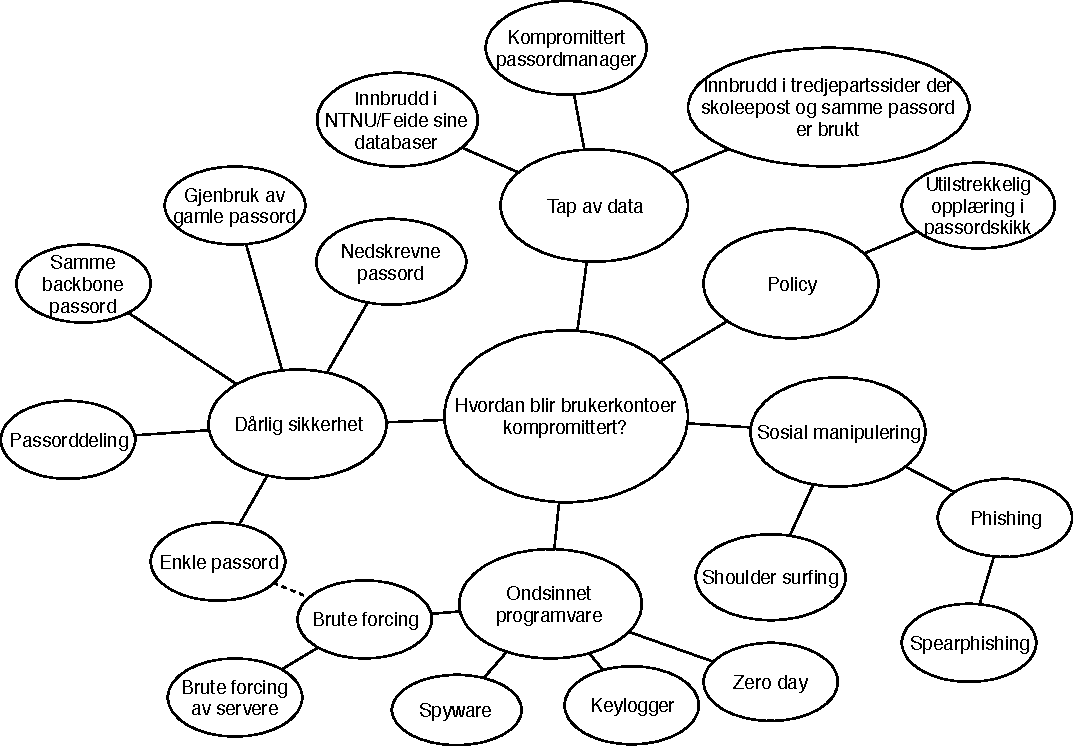
\includegraphics[scale=0.6]{case_2/bilder/idemyldring.pdf}
    \caption[Idémyldring for kompromitterte kontoer]{Resultater og gruppering av idémyldringen}
    \label{fig:case2-idemyldring}
\end{figure}

Resultatene er gruppert inn i 4 hovedkategorier:
\begin{description}
    \item [Dårlig sikkerhet] er alt fra enkle passord til passordgjenbruk.
    \item [Tap av data] inkluderer at for eksempel sider som dropbox har en lekkasje av brukerinformasjon.
    \item [Sosial manipulering] vil si å få tak i informasjon ved å lure noen.
    \item [Ondsinnet programvare] er programvare brukt som hjelpemiddel for å få tak i brukerinformasjon.
\end{description}

\section{Datainnsamling}
Under idémyldringen ble det avdekket en rekke faktorer som kunne være medvirkende i at ansatte og studenter ved NTNU fikk sin konto på avveie. Vi brukte denne informasjonen aktivt da spørreundersøkelsen ble konstruert. Spørreundersøkelsen slik den fremstår for respondenten finnes i vedlegg \ref{undersokelse_norsk}. Når spørsmålene ble laget ble det bestemt hypoteser til spørsmålene. Disse er listet i tabell \ref{tab:case2-hypoteser} under. 

% Table generated by Excel2LaTeX from sheet 'Ark2'
\begin{table}[H]
  \centering
  \caption{Hypoteser til spørsmålene for kompromitterte kontoer}
    \begin{tabular}{|p{20.215em}|p{20.57em}|}
    \hline
    \rowcolor{yellow} Spørsmål & Hypoteser \\
    \hline
    Din alder? & Eldre er overrepresentert i statistikken over tapte kontoer \\
    \hline
    Ditt kjønn? & Flere kvinner enn menn har blitt kompromittert \\
    \hline
    Hva er din primærrolle ved NTNU? & Det er ansatte som er målgruppen til trusselaktørene \\
    \hline
    I hvilken by jobber/studerer du primært? & Gjøvik har høyere sikkerhetskompetanse \\
    \hline
    I hvor mange år har du jobbet/studert ved NTNU eller de tidligere høgskolene? & Folk med lavere ansiennitet kjenner universitetets retningslinjer bedre \\
    \hline
    Når fant du ut at NTNU kontoen din var blitt kompromittert? & Folk vet ikke at de har blitt kompromittert før de blir kontaktet \\
    \hline
    Har du noen formening om hvor lang tid kontoen var kompromittert før Seksjon for Digital Sikkerhet kontaktet deg? & Ingen hypotese grunnet vagt spørsmål \\
    \hline
    Har du noen formening om hvordan kontoen din ble kompromittert? & Ingen hypotese grunnet åpent svar \\
    \hline
    Bruker du din NTNU e-post til å registrere deg på ulike tjenester på nett i forbindelse med jobben/studiet? & Over halvparten bruker NTNU e-post til tjenester i forbindelse med jobb \\
    \hline
    Bruker du din NTNU e-post til å registrere deg på tjenester på nett til privat bruk? & Under halvparten bruker NTNU e-post til privat bruk \\
    \hline
    På en skala fra 1-6, der 1 er lite bevisst og 6 er svært bevisst, hvor bevisst er du på sikkerhet når du... & \multirow{4}[2]{*}{Folk er generelt sett lite bevisste} \\
    besøker nettsider? & \multicolumn{1}{r|}{} \\
    lager passord? & \multicolumn{1}{r|}{} \\
    sjekker e-post? & \multicolumn{1}{r|}{} \\
    \hline
    Har du i din tid hos NTNU lagt merke til phishing-forsøk mot deg på din NTNU e-post? & Phishing er en svært utbredt angrepsvektor \\
    \hline
    Har du blitt lurt av phishing på din NTNU e-post? & Av de som har blitt kompromittert har under en tredjedel blitt lurt av phishing \\
    \hline
    Har du i løpet av din tid ved NTNU eller de andre høgskolene, oppdaget virus eller annen skadevare på maskinen din? & Virus og annen skadevare er utbredt \\
    \hline
    Bruker du ditt NTNU passord på flere tjenester? & Passordgjenbruk er utbredt \\
    \hline
    Brukte du regler til å generere ditt NTNU passord? & De fleste bruker ikke passordregler til å generere passord \\
    \hline
    Er ditt NTNU passord tilfeldig sammensatt av bokstaver, tall og/eller tegn? & De fleste bruker ikke tilfeldig sammensatte passord \\
    \hline
    Hvor mange tegn består ditt NTNU passord av? & Over halvparten har passord på under 12 tegn \\
    \hline
    Har du i løpet av din tid ved NTNU delt NTNU passordet ditt med andre? & Passorddeling er ikke særlig utbredt \\
    \hline
    Omtrent hvor ofte bytter du ditt NTNU passord? & Passord byttes for det meste sjeldnere enn hvert andre år \\
    \hline
    Bruker du en passordmanager? & De fleste bruker ikke passordmanager, og mange vet ikke engang hva det er \\
    \hline
    På en skala fra 1 til 6, hvor godt kjent er du med... & \multirow{4}[2]{*}{Det er svært lite kjennskap til retningslinjer} \\
    NTNU sine retningslinjer for behandling av brukernavn, passord og andre autentiseringsdata? & \multicolumn{1}{r|}{} \\
    IT reglementet til NTNU? & \multicolumn{1}{r|}{} \\
    NTNU sine prinsipper for informasjonssikkerhet? & \multicolumn{1}{r|}{} \\
    \hline
    Har du fått opplæring i passordsikkerhet fra NTNU? & Under en fjerdedel har fått opplæring i passordskikk fra NTNU \\
    \hline
    \end{tabular}%
  \label{tab:case2-hypoteser}%
\end{table}%

Av de som e-posten ble sendt ut til fikk vi totalt 72 gyldige respondenter, mens 26 stoppet rett etter åpning av undersøkelsen eller underveis. Undersøkelsen var aktiv i perioden fra 20. April til og med 27. April. I løpet av denne tiden ble det sendt ut én purring den 25. April. 

\section{Dataanalyse}
I denne fasen analyseres dataene som er samlet inn, og ved hjelp av statistiske verktøy kan vi trekke konklusjoner basert på svarene. Verktøyet vi bruker til å utføre mesteparten av analysene er SPSS.

\subsection{Svarstatistikk}
Spørreundersøkelsen ble mottatt av 157 personer som har fått kontoen kompromittert. Av disse var det 72 som svarte. Det var i tillegg 26 som startet spørreundersøkelsen, men ikke fullførte. Figur \ref{fig:case2-svar-per-dag} under viser statistikk over hvor mange svar som kom inn per dag.

\begin{figure}[H]
    \centering
    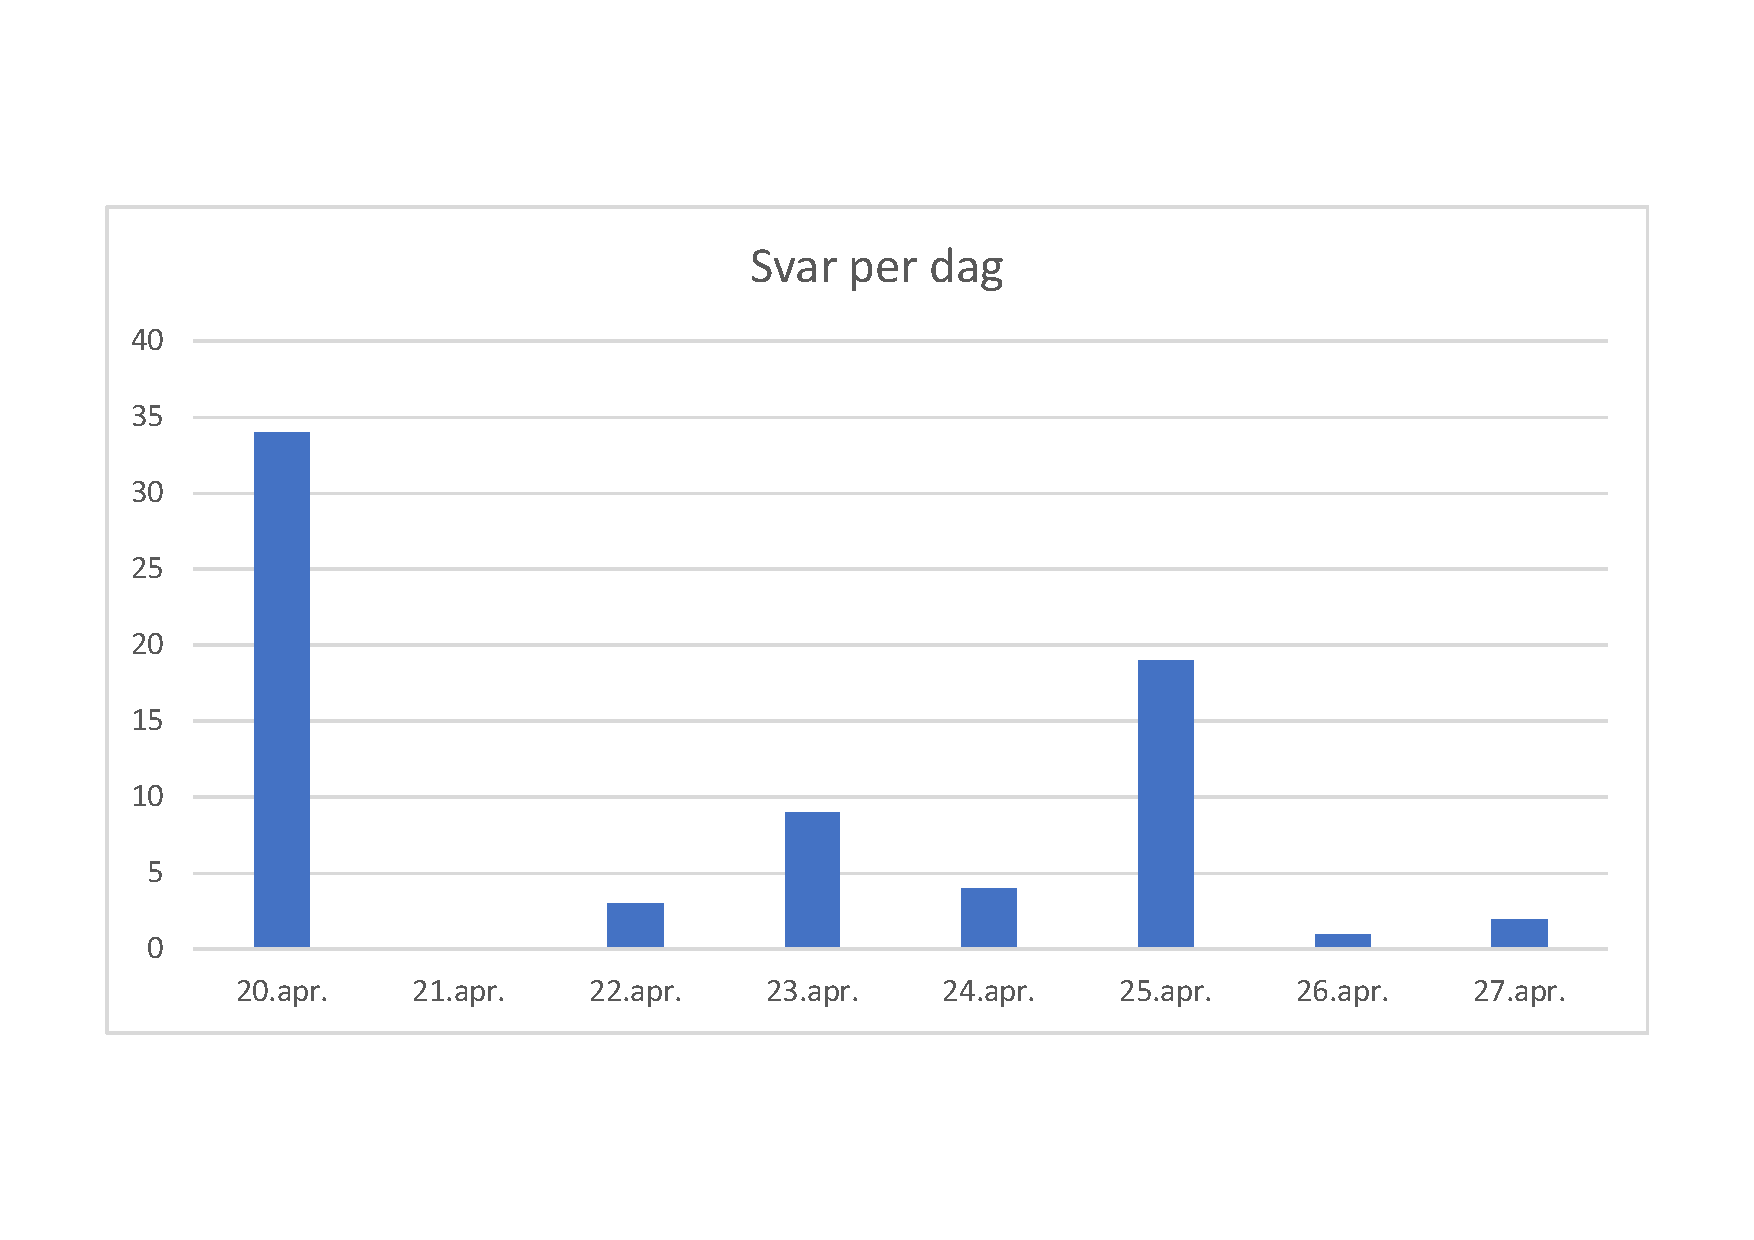
\includegraphics[scale=0.5, clip, trim=1cm 3cm 0cm 3cm]{case_2/bilder/spss/svar_per_dag.pdf}
    \caption[Svar per dag]{Antall svar vi fikk per dag}
    \label{fig:case2-svar-per-dag}
\end{figure}

Det var tydelig mest svar dagen spørreundersøkelsen ble lansert, og 25. April, hvor vi sendte ut en purre e-post. Det bør nevnes at undersøkelsen ble sendt ut på en fredag, og 21. og 22. April var en lørdag og søndag. Derfor gikk antall svar litt opp igjen på mandag 23. April. 

\subsection{Demografi}
I denne delen fremlegges resultatene fra demografien i spørreundersøkelsen. Disse blir om mulig sammenliknet med generelle tall fra NTNU for å få et innblikk i demografien til de som har blitt kompromittert, kontra NTNU sine ansatte og studenter generelt. Vi fokuserer stort sett på de ansatte siden antall studenter i undersøkelsen var få.

\subsubsection{Aldersgruppe}
Aldersgruppene ble kategorisert i intervaller på 10 år. Fra de ulike kategoriene fikk vi:

\begin{itemize}
    \item Under 20: 1 person
    \item 20-29: 3 personer
    \item 30-39: 13 personer
    \item 40-49: 27 personer
    \item 50-59: 11 personer
    \item 60-69: 9 personer
    \item 70 eller over: 8 personer
\end{itemize}

Under ser vi aldersfordelingen visuelt fremstilt i et histogram.

\begin{figure}[H]
    \centering
    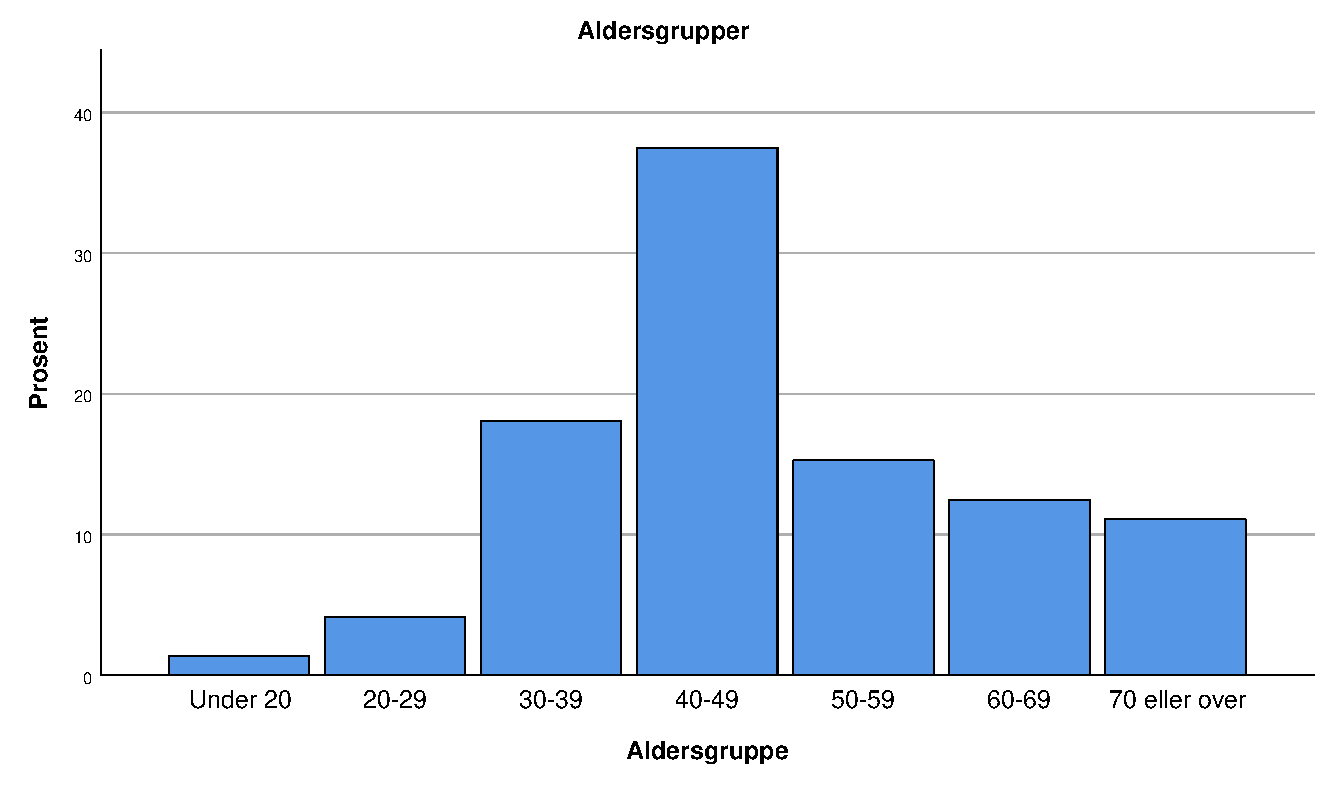
\includegraphics[scale=0.5]{case_2/bilder/spss/aldersgrupper.pdf}
    \label{fig:case2-aldersgruppe}
    \caption[Aldersgrupper av de kompromitterte]{Aldersgrupper av respondentene}
\end{figure}

Ut fra resultatene kan vi konkludere med at de som har blitt kompromittert er stort sett middelaldrene til eldre personer. Disse personene er også noe eldre enn gjennomsnittsalderen til de som jobber ved NTNU \cite{MorkRapport}. 

\subsubsection{Kjønn}
Av de 72 respondentene var det 45 kvinner og 27 menn. Det er henholdsvis 62,5\% og 37,5\%. Under er kjønnsfordelingen visualisert i et sektordiagram.

\begin{figure}[H]
    \centering
    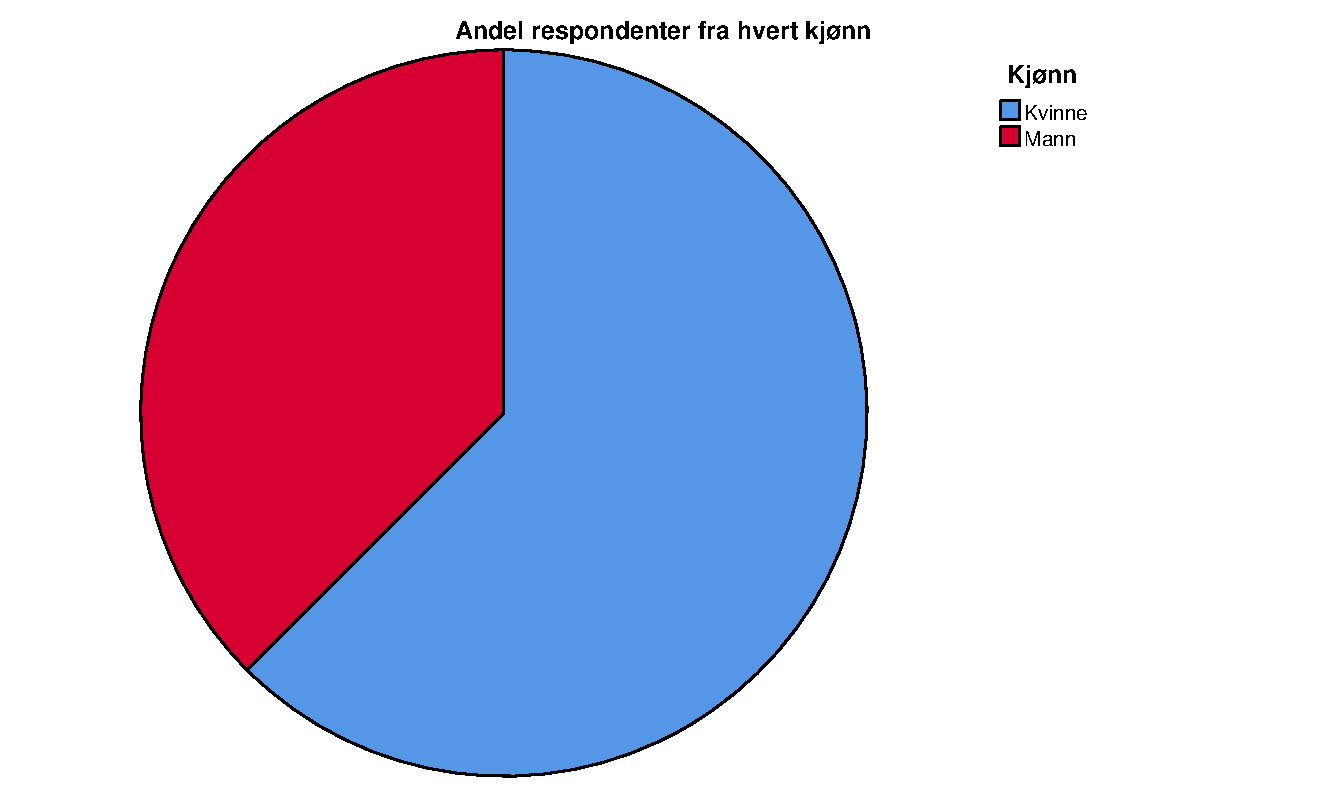
\includegraphics[scale=0.5]{case_2/bilder/spss/kjonn.pdf}
    \label{fig:case2-kjonn}
    \caption[Andel fra hvert kjønn av de kompromitterte]{Andel fra hvert kjønn}
\end{figure}

De fleste av de som har svart er kvinner. Av de ansatte ved NTNU er det 41\% kvinner totalt \cite{NTNUfakta}. Totalt sendte vi ut spørreundersøkelsen til 167 e-postadresser, der 157 av de mottok. Vi har tall på at 91 av de 167 vi først sendte ut til var kvinner. Dette er omtrent 55\%. For å kunne si noe om antallet kvinner som svarte på spørreundersøkelsen må vi se på om svarene våre er representative for hele samplet. Vi brukte en kalkulator for å regne ut konfidensintervallet for vårt sample \cite{SSCalc}. Utregningen kom fram til at vi er 95\% sikre på at feilmarginen for dette spørsmålet er \(\pm 8,5\%\). I og med at andelen kvinner totalt på NTNU er 41\%, kan vi fastslå at kvinner er noe mer utsatt for å få kontoen kompromittert, men denne forskjellen er ikke stor.

\subsubsection{Primærrolle}
Av de 72 respondentene var det 6 studenter og 66 ansatte. Dette er henholdsvis 8,3\% og 91,7\%. Sektordiagrammet under viser fordelingen.

\begin{figure}[H]
    \centering
    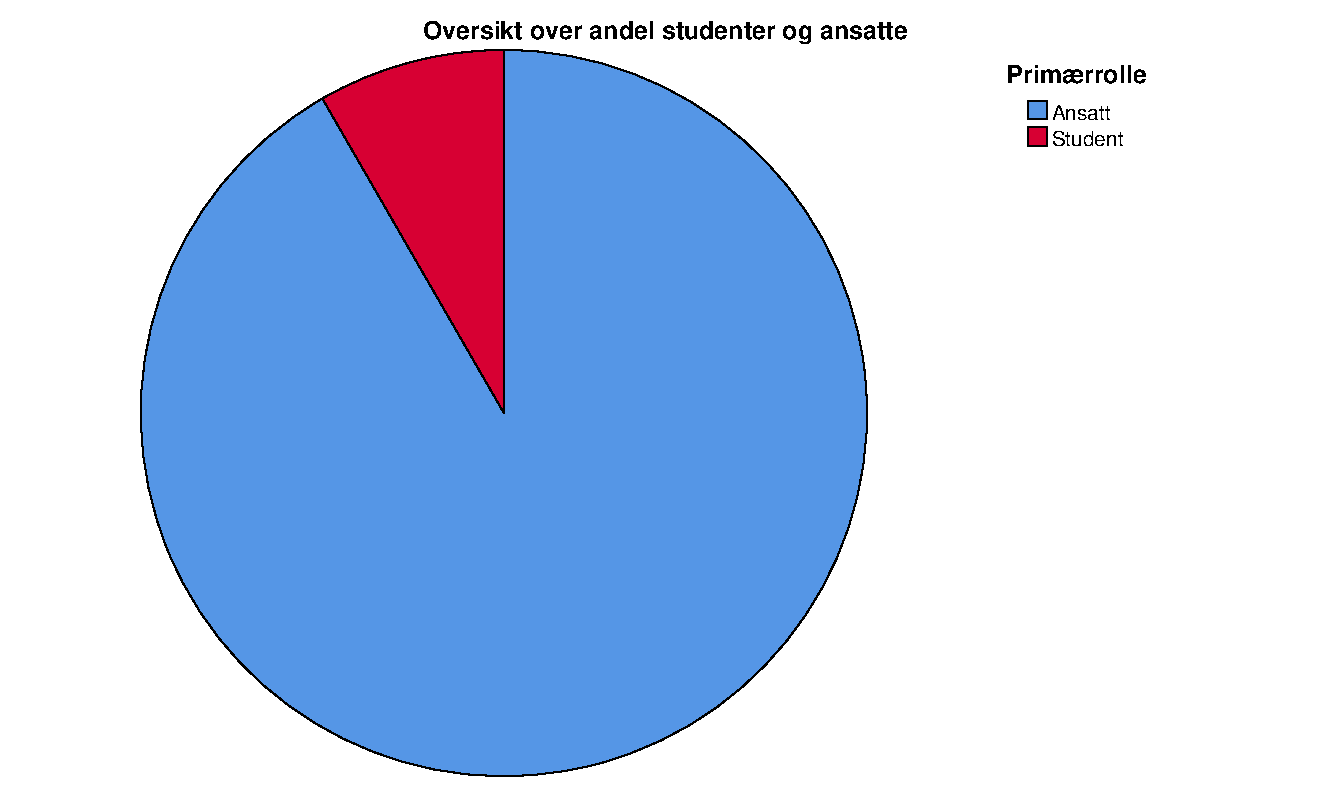
\includegraphics[scale=0.5]{case_2/bilder/spss/primaerrolle.pdf}
    \label{fig:case2-primaerrolle}
    \caption[Primærrolle ved NTNU]{Primærrolle ved NTNU}
\end{figure}

Fra dataene kan vi se at ansatte er overrepresentert i de som blir kompromittert. Vi har data på at det er 18 studenter i vårt sample, altså står studenter for omtrent 10\% av de kompromitterte. På samme måte som i forrige seksjon, ble konfidensintervallet regnet ut \cite{SSCalc}. Utregningen kom frem til at vi er 95\% sikre på at feilmarginen er på \(\pm 5,12\%\). Det er desidert flere studenter enn ansatte ved NTNU \cite{NTNUfakta}. Derfor kan vi med høy sikkerhet si at trusselaktørenes målgruppe er de ansatte og ikke studenter. 

\subsubsection{Primærby}
Av de 72 respondentene var det bare en fra Ålesund og resten var fra Trondheim. Det var ingen respondenter fra Gjøvik. 

\subsubsection{År ved NTNU}
Bare 6 personer, eller 8,3\% av respondentene hadde jobbet eller studert ved NTNU i under 2 år og i 2 til 4 år. 9 personer, eller 12,5\% hadde jobbet eller studert her i 5 til 9 år, og 15 personer, eller 20,8\% hadde jobbet eller studert her i 10 til 15 år. Hele 36 personer, eller akkurat halvparten av respondentene har vært hos NTNU i over 15 år. En oversikt over disse tallene finnes i histogrammet under. 

\begin{figure}[H]
    \centering
    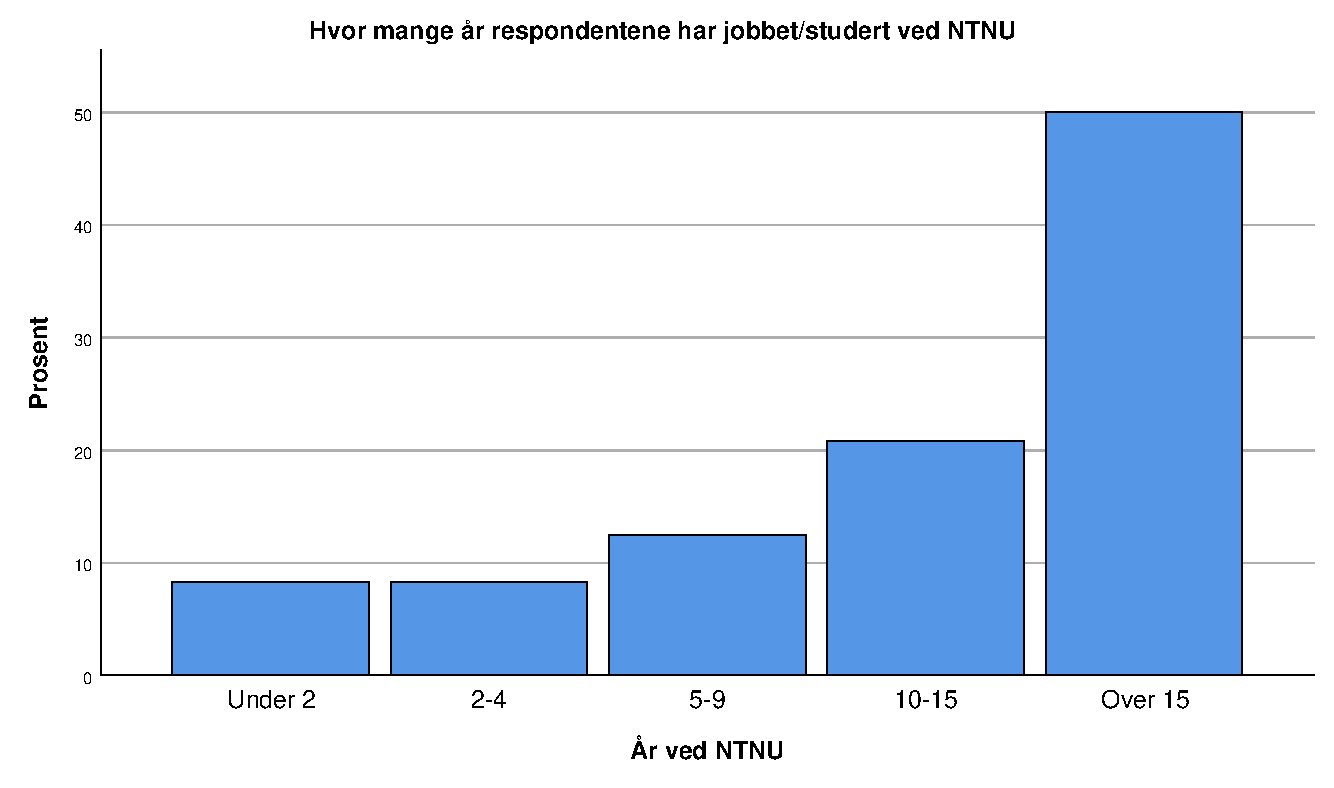
\includegraphics[scale=0.5]{case_2/bilder/spss/aarvedNTNU.pdf}
    \label{fig:case2-aarvedNTNU}
    \caption[Antall år ved NTNU]{Antall år ved NTNU}
\end{figure}

\subsection{Bevissthet på sikkerhet}
Spørsmålene skulle gi svar på hvor sikkerhetsbevisst en tenker når man besøker nettsider, lager passord og sjekker e-post. Hypotesen som ble fremhevet her var at folk generelt sett er lite bevisste. 

Histogrammet i figur \ref{fig:case2-bevisst-nettsider} viser en tilnærmet normalfordelt situasjon, men med noe fler svar på høyresiden. De fleste er derfor litt mer bevisste på sikkerhet når de besøker nettsider enn de er ubevisste. 
\begin{figure}[H]
    \centering
    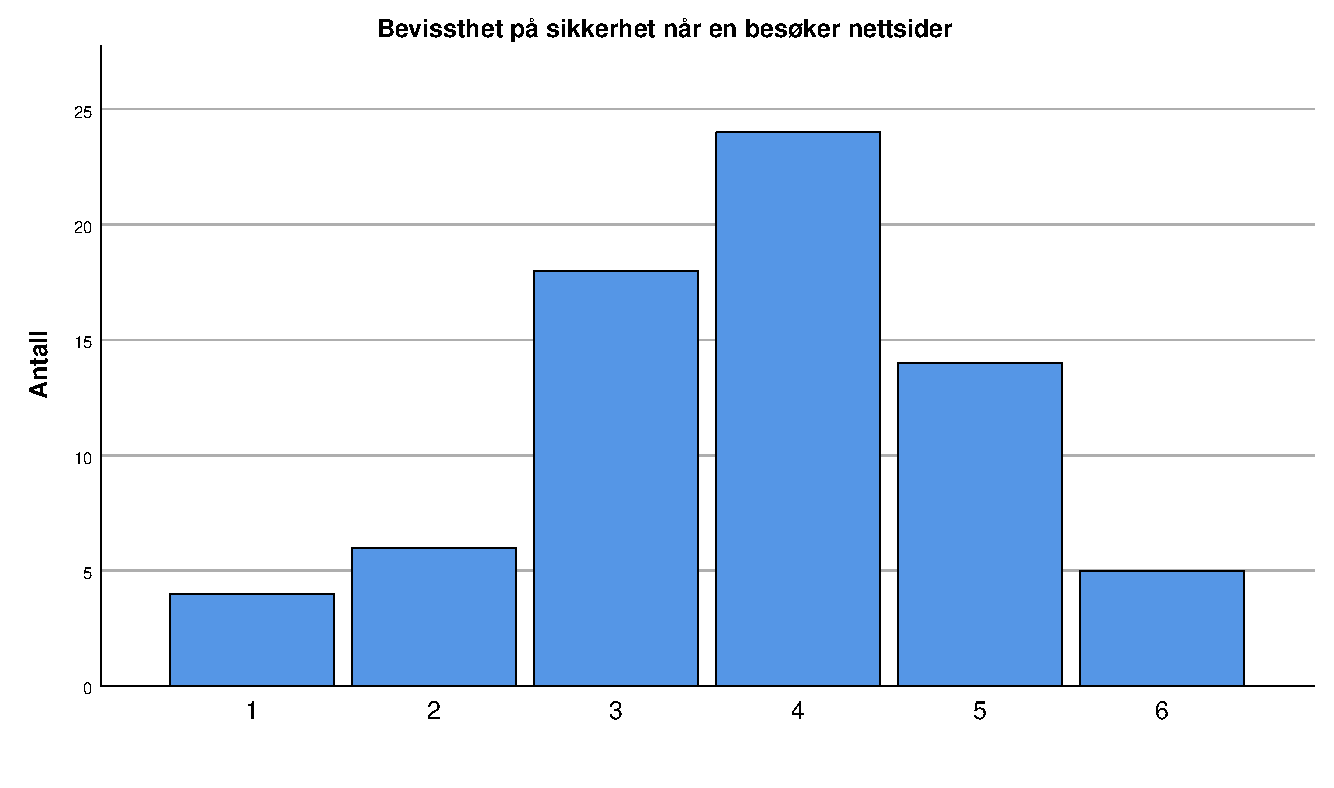
\includegraphics[scale=0.5]{case_2/bilder/spss/bevisst_nettsider.pdf}
    \caption[Bevisst på sikkerhet med nettsider]{Bevissthet på sikkerhet når en besøker nettsider}
    \label{fig:case2-bevisst-nettsider}
\end{figure}

Når det kommer til sikkerhet når en lager passord svarer respondentene at de generelt sett er bevisste på dette. Figur \ref{fig:case2-bevisst-passord} under viser at fordelingen er konsentrert hovedsaklig på høyresiden.
\begin{figure}[H]
    \centering
    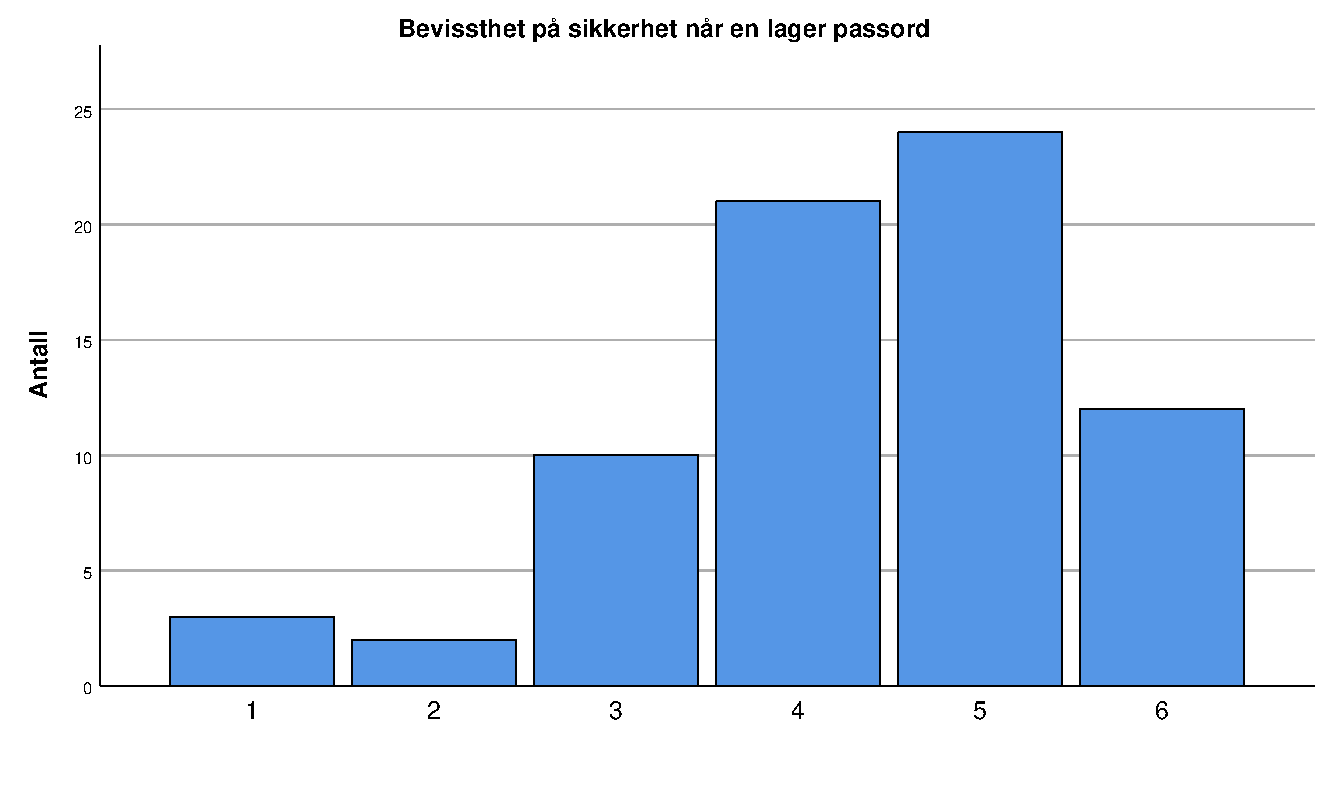
\includegraphics[scale=0.5]{case_2/bilder/spss/bevisst_passord.pdf}
    \caption[Bevisst på sikkerhet med passord]{Bevissthet på sikkerhet når en lager passord}
    \label{fig:case2-bevisst-passord}
\end{figure}

Figur \ref{fig:case2-bevisst-e-post} under viser bevissthetsfordelingen når det kommer til sjekking av e-post. Dette var noe vi spesielt ønsket å se på siden en av hovedhypotesene våre til kompromitterte brukerkontoer er phishing. Histogrammet viser at respondentene stort sett er bevisste på sikkerhet når de sjekker e-post.
\begin{figure}[H]
    \centering
    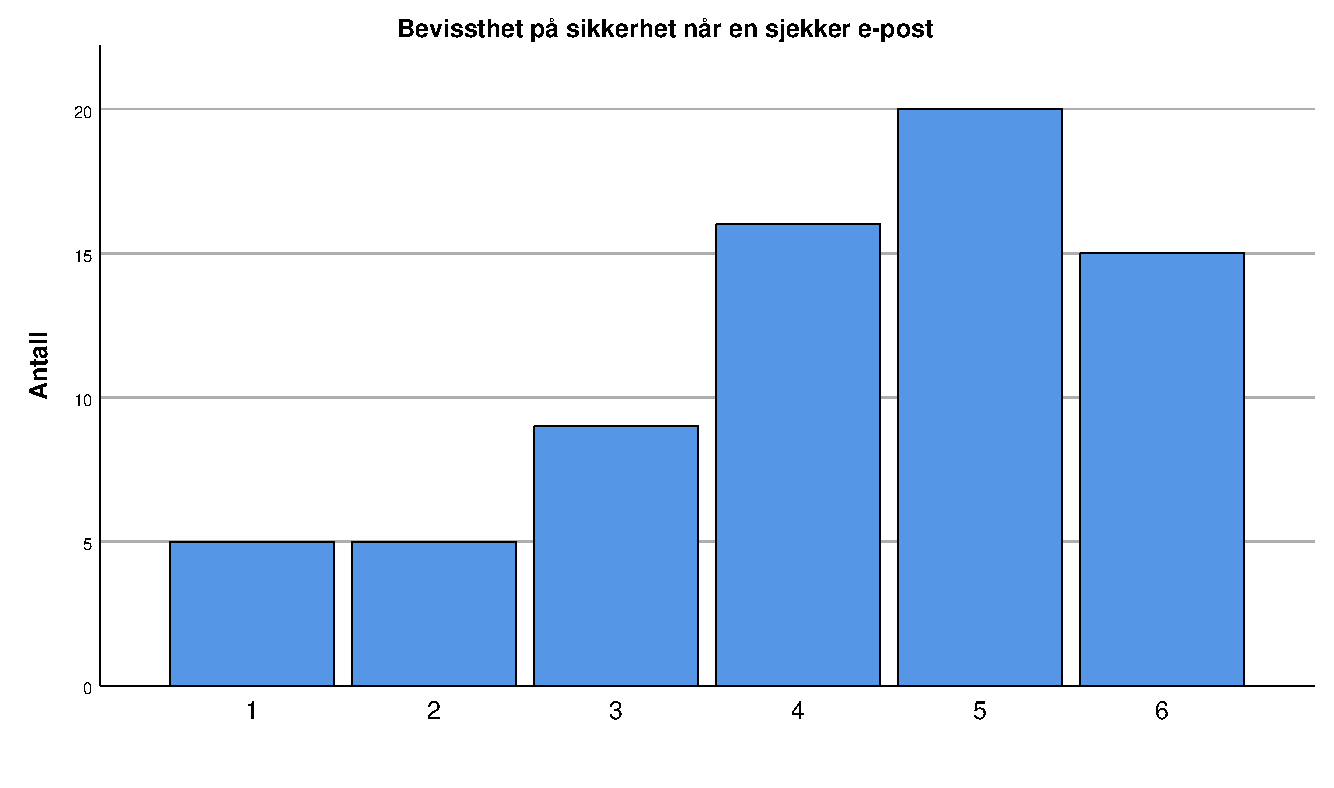
\includegraphics[scale=0.5]{case_2/bilder/spss/bevisst_e-post.pdf}
    \caption[Bevisst på sikkerhet med e-post]{Bevissthet på sikkerhet når en sjekker e-post}
    \label{fig:case2-bevisst-e-post}
\end{figure}

\subsection{Kjennskap til retningslinjer, reglementer og prinsipper}
Disse spørsmålene handler om hvor godt kjennskap respondentene har til NTNU sine retningslinjer for behandling av autentiseringsdata, IT reglementet og prinsipper for informasjonssikkerhet. Hypotesen vi hadde her var at de aller fleste hadde lite kjennskap til disse.

Det viser seg fra figur \ref{fig:case2-retningslinjer} at respondentene kan lite om NTNU sine retningslinjer for behandling av brukernavn, passord og andre autentiseringsdata. 
\begin{figure}[H]
    \centering
    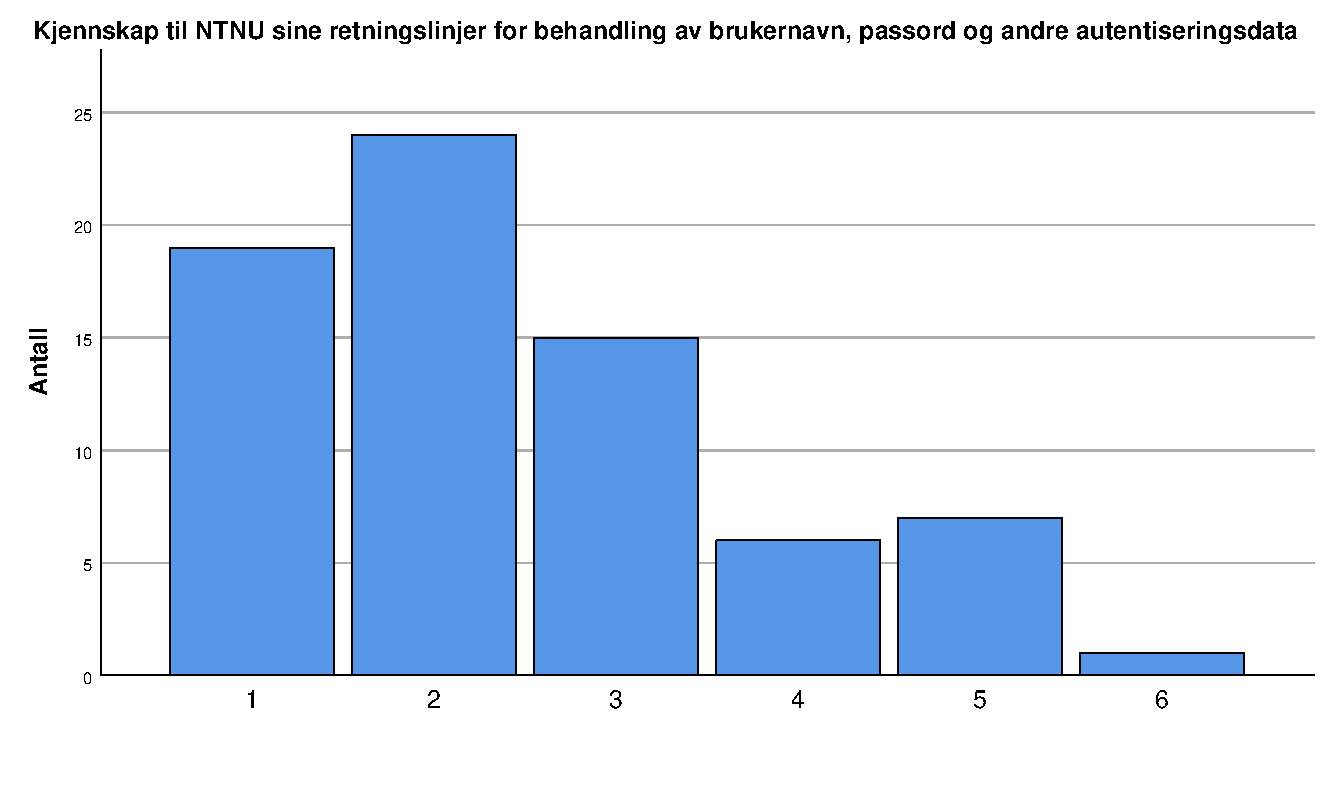
\includegraphics[scale=0.5]{case_2/bilder/spss/retningslinjer.pdf}
    \caption[Kjennskap til retningslinjer]{Kjennskap til retningslinjer}
    \label{fig:case2-retningslinjer}
\end{figure}

Figur \ref{fig:case2-ITreglement} viser at respondentene ikke kjenner så godt til IT reglementet til NTNU. Over 70\% svarte 3 eller under på hvor godt de kjente IT reglementet til NTNU, der 1 var lite kjent og 6 var meget kjent.  
\begin{figure}[H]
    \centering
    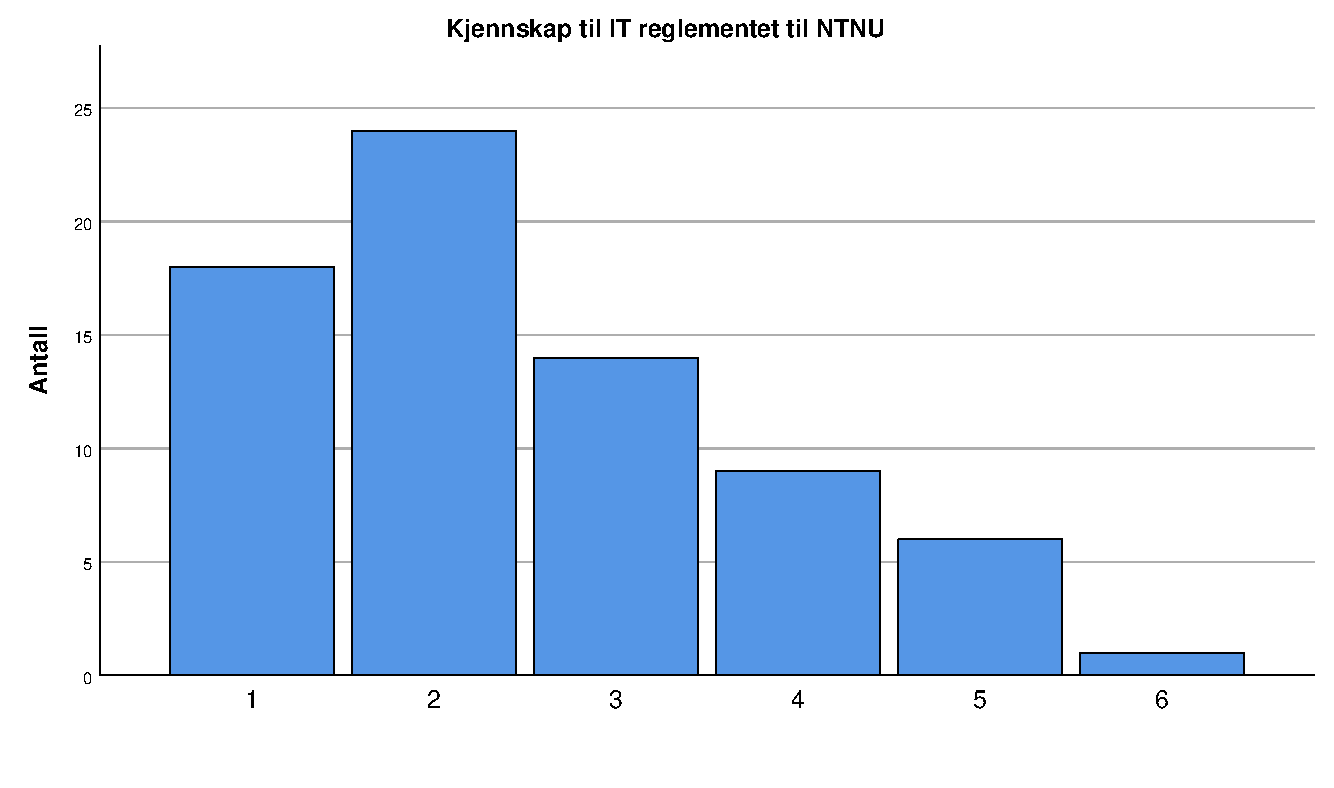
\includegraphics[scale=0.5]{case_2/bilder/spss/ITreglement.pdf}
    \caption[Kjennskap til IT-reglement]{Kjennskap til IT reglement}
    \label{fig:case2-ITreglement}
\end{figure}

Under viser figur \ref{fig:case2-InfoSecPolicy} at folk har dårlig kjennskap til NTNU sine prinsipper for informasjonssikkerhet. Der står det blant annet at brukere er ansvarlige for enhver bruk av innloggingskredentialier og at de holder dette konfidensielt \cite{PrinsInfoSec}. 
\begin{figure}[H]
    \centering
    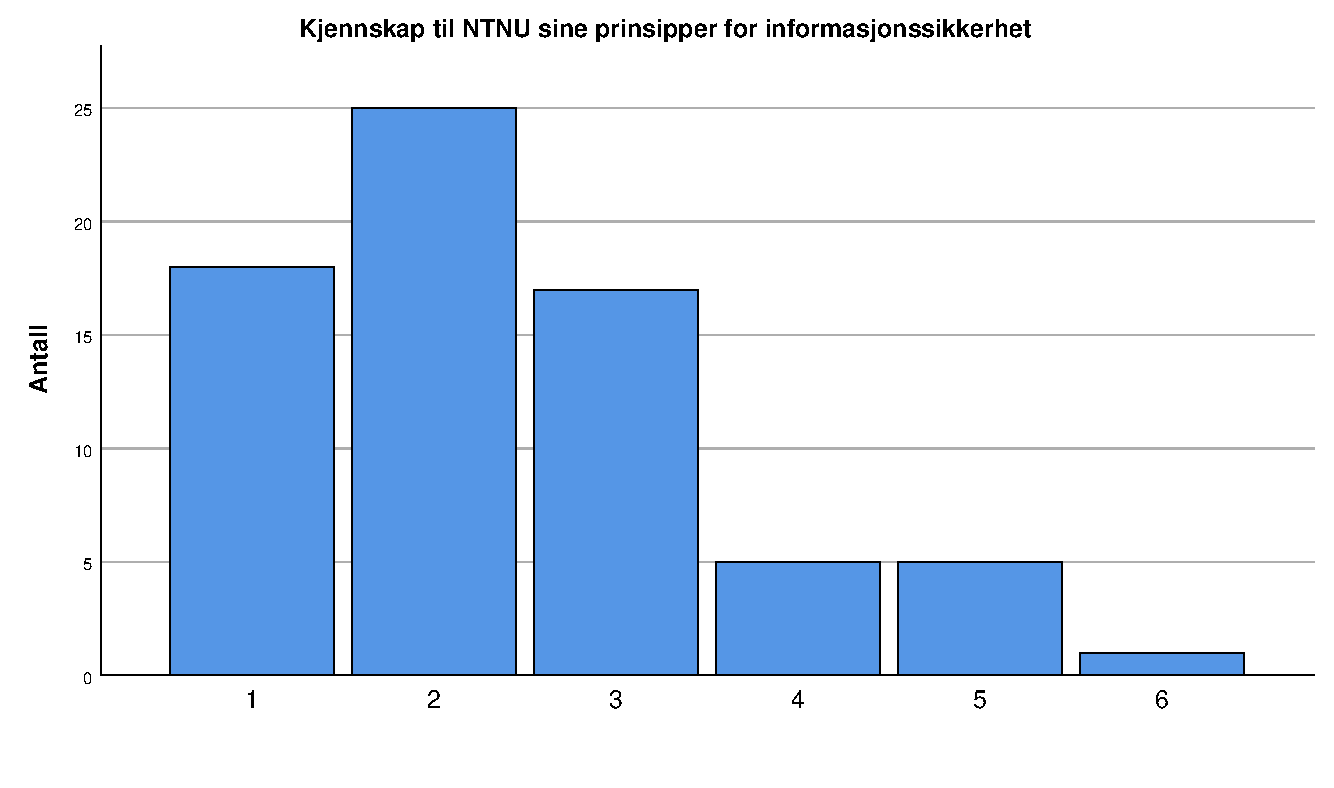
\includegraphics[scale=0.5]{case_2/bilder/spss/InfoSecPolicy.pdf}
    \caption[Kjennskap til prinsipper for informasjonssikkerhet]{Kjennskap til NTNU sine prinsipper for informasjonssikkerhet}
    \label{fig:case2-InfoSecPolicy}
\end{figure}

Det viser seg at hypotesen vi hadde stemte. Det er lite kjennskap til styringsdokumentene.

\subsection{Respondentenes egen oversikt}
Over 60\% av respondentene viste ikke at kontoen var blitt kompromittert før Seksjon for Digital Sikkerhet ringte, og kun 20\% svarte at de fant ut av det før og resten svarte at de ikke vet.

\begin{figure}[H]
    \centering
    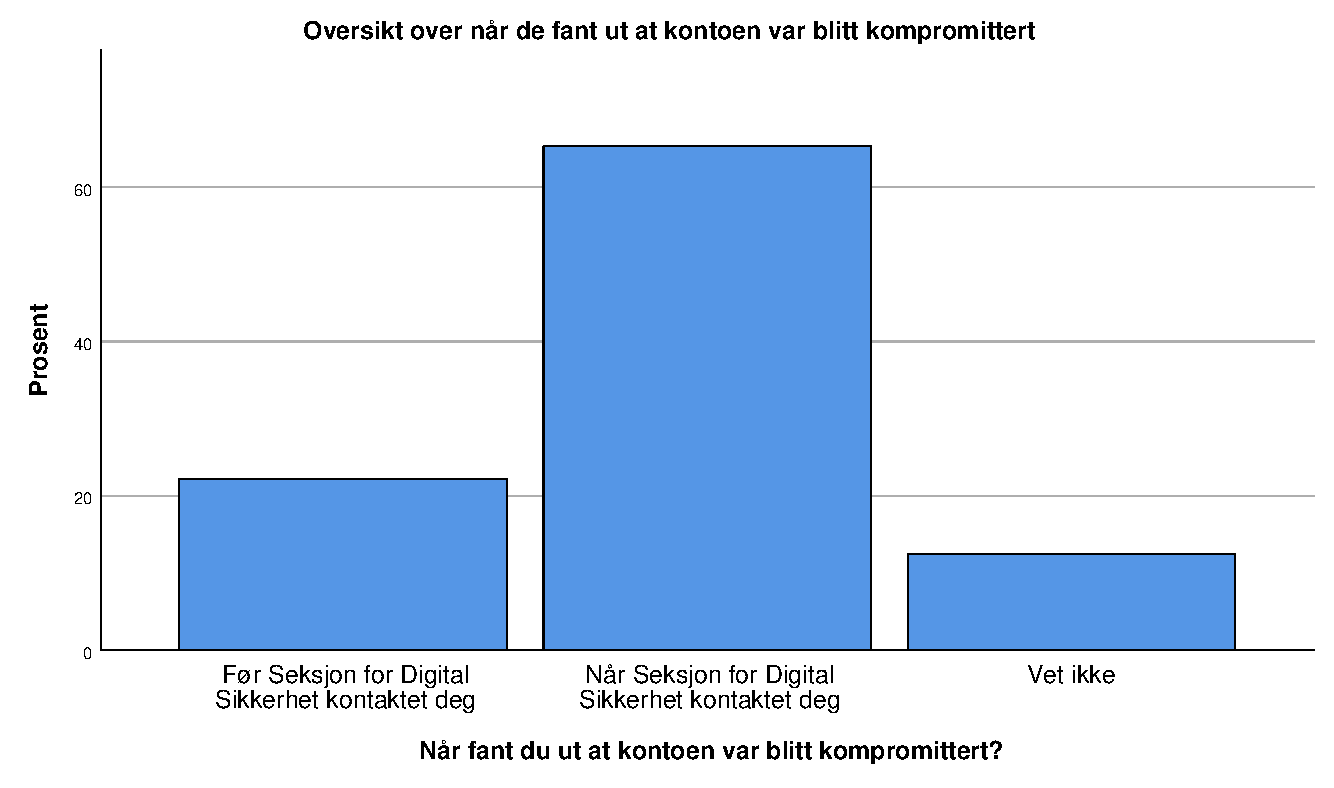
\includegraphics[scale=0.5]{case_2/bilder/spss/Fant_ut_kompromittert.pdf}
    \caption[Når de fant ut de var kompromittert]{Viser når de fant ut at de var blitt kompromittert}
    \label{fig:case2-fant-ut-kompromittert}
\end{figure}

Hypotesen vår her var korrekt. De vet ikke at de har blitt kompromittert før de blir kontaktet.

Respondentene svarte at de trodde kontoen var kompromittert mindre enn tre måneder før Seksjon for Digital Sikkerhet kontaktet dem, som vist i figur \ref{fig:fant-ut-kompromittert}. Denne statistikken kan vi ikke være helt sikre på, fordi halvveis i undersøkelsen fikk vi tilbakemeldiner på at det var flere som ikke ville fullføre spørreundersøkelsen siden dette svaret var obligatorisk og det ikke var noe alternativ for ``vet ikke''. Vi fjernet da kravet om å svare halvveis ut i undersøkelsen.
\begin{figure}[H]
    \centering
    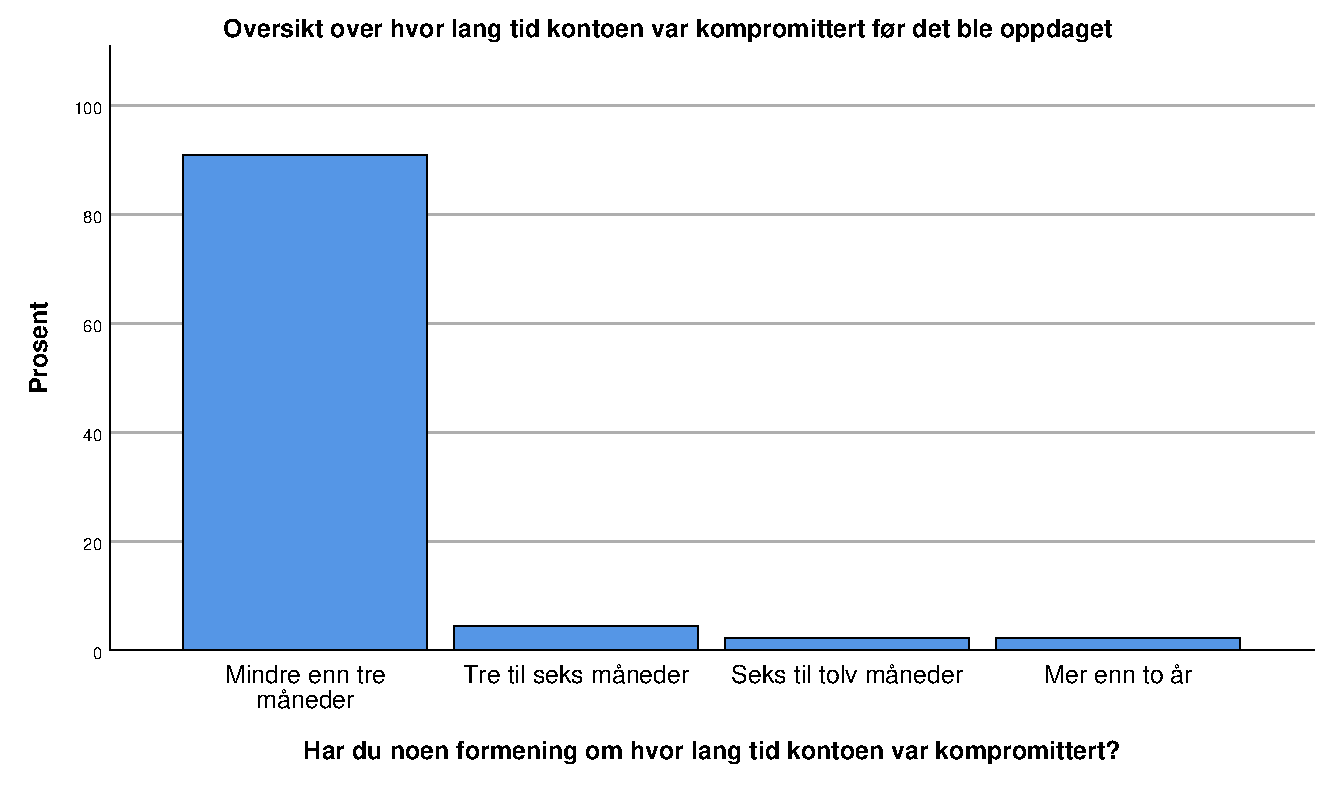
\includegraphics[scale=0.5]{case_2/bilder/spss/lang_tid_konto_kompromittert.pdf}
    \caption[Hvor lang tid de tror de var kompromittert]{Viser hvor lang tid de tror de var kompromittert}
    \label{fig:fant-ut-kompromittert}
\end{figure}

\subsubsection{Formening om hvordan det skjedde}
Affinitetsdiagramet viser at respondentene i hovedsak ikke har noen formening om hvordan kontoen ble kompromittert. Over 85\% svarte at de ikke hadde noen formening om hvordan kontoen ble kompromittert.
\begin{figure}[H]
    \centering
    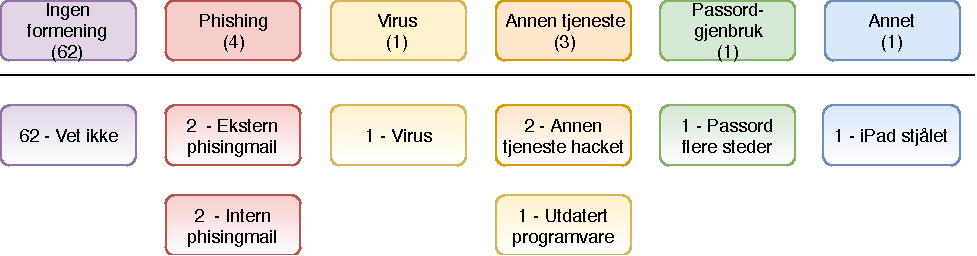
\includegraphics[scale=0.8]{case_2/bilder/Affinitetsdiagram.pdf}
    \caption[Affinitetsdiagram av formening om hvordan det skjedde]{Affinitetsdiagram av respondentenes formening over hvordan kontoen ble kompromittert}
    \label{fig:case2-affinitetsdiagram}
\end{figure}

\subsection{Bruker- og passordvaner}
Som vi kan se i figur \ref{fig:case2-epost-jobb} under, bruker over 60\% av respondentene NTNU e-posten til å registrere seg på tjenester i forbindelse med jobb.
\begin{figure}[H]
    \centering
    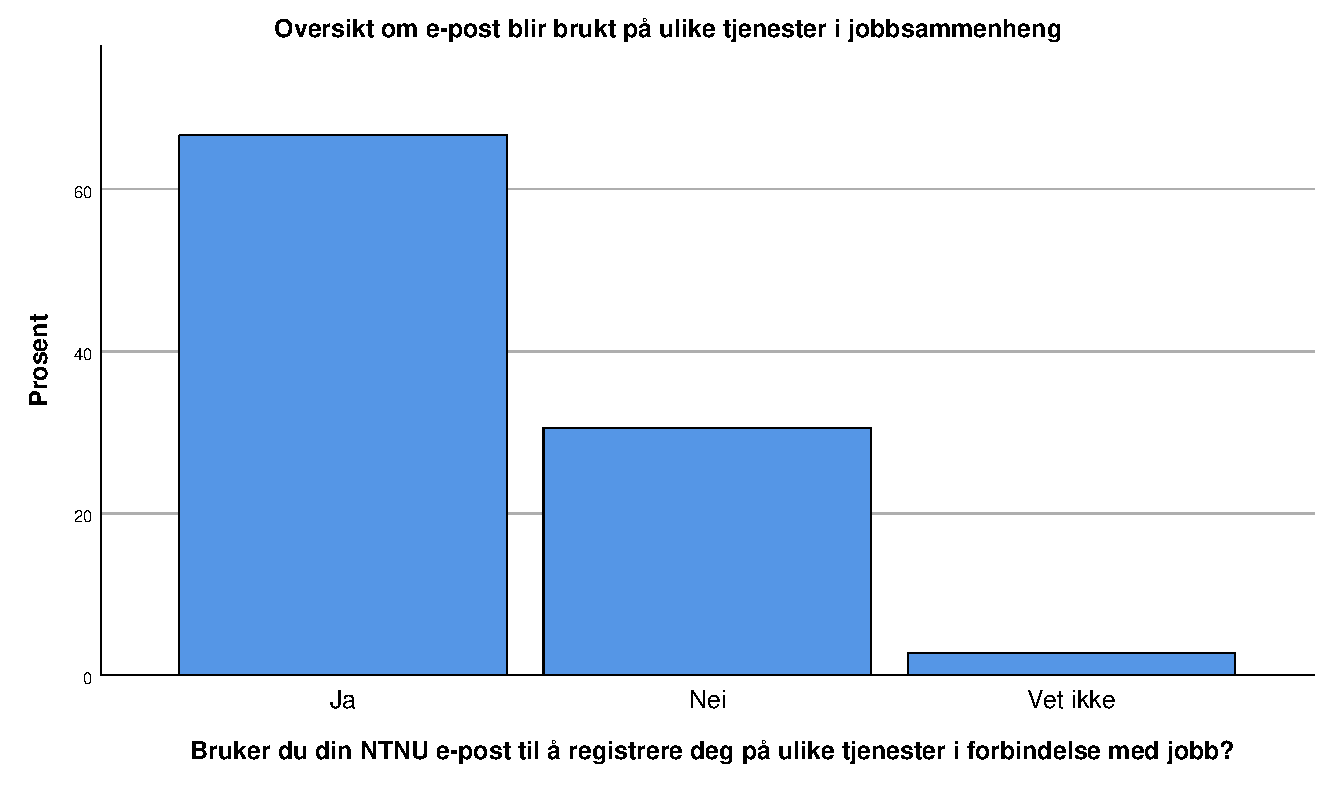
\includegraphics[scale=0.5]{case_2/bilder/spss/epost_jobb.pdf}
    \caption[E-post til jobbrelaterte tjenester]{Viser hvor mange som bruker NTNU e-post til andre jobbrelaterte tjenester}
    \label{fig:case2-epost-jobb}
\end{figure}

48,6\% av respondentene bruker NTNU e-posten sin til private tjenester. Den samme andelen gjør ikke det og de restende (2,8\%) har svart at de ikke vet. Dette blir vist i figur \ref{fig:case2-epost-privat}.
\begin{figure}[H]
    \centering
    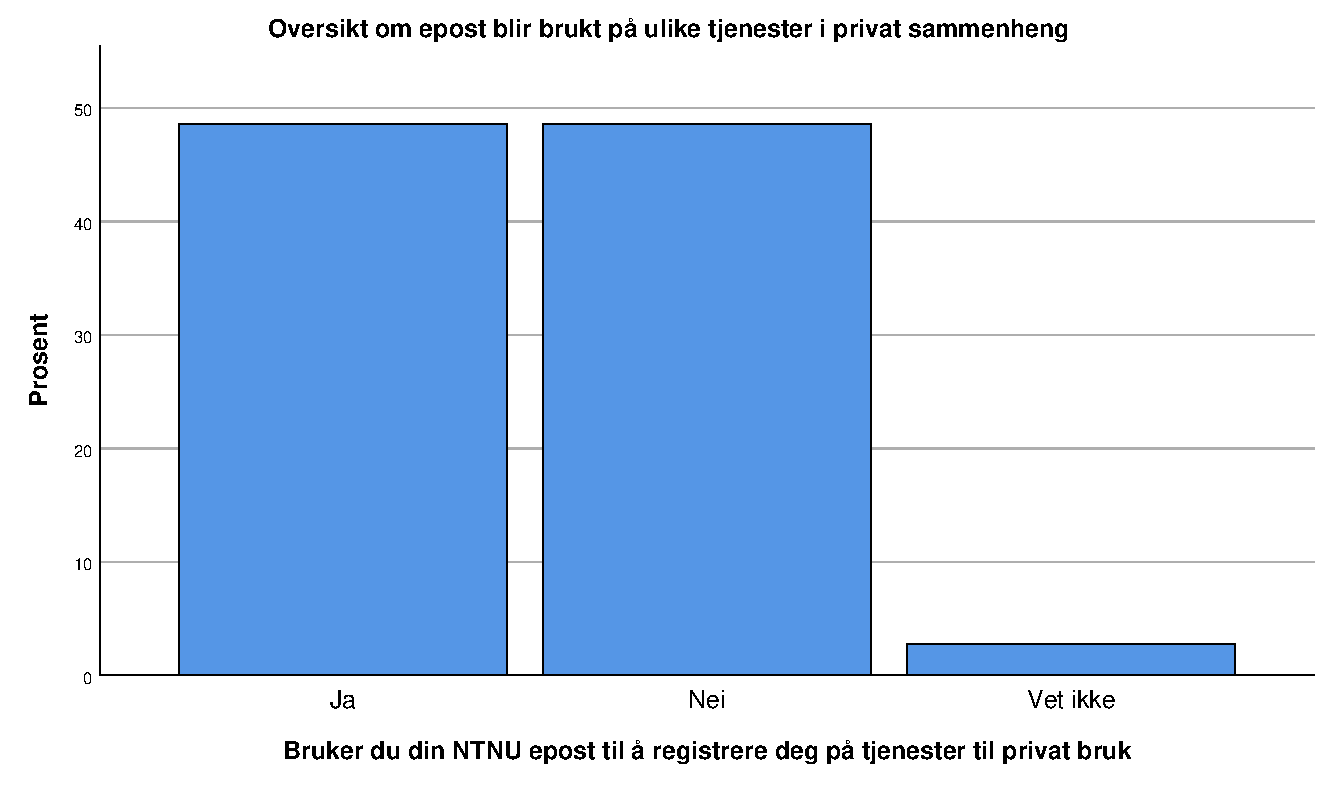
\includegraphics[scale=0.5]{case_2/bilder/spss/epost_privat.pdf}
    \caption[E-post til private tjenester]{Viser hvor mange som bruker NTNU e-post til private tjenester}
    \label{fig:case2-epost-privat}
\end{figure}

Over 50\% av respondentene bruker NTNU passordet på flere tjenester som vist i figuren under. 
\begin{figure}[H]
    \centering
    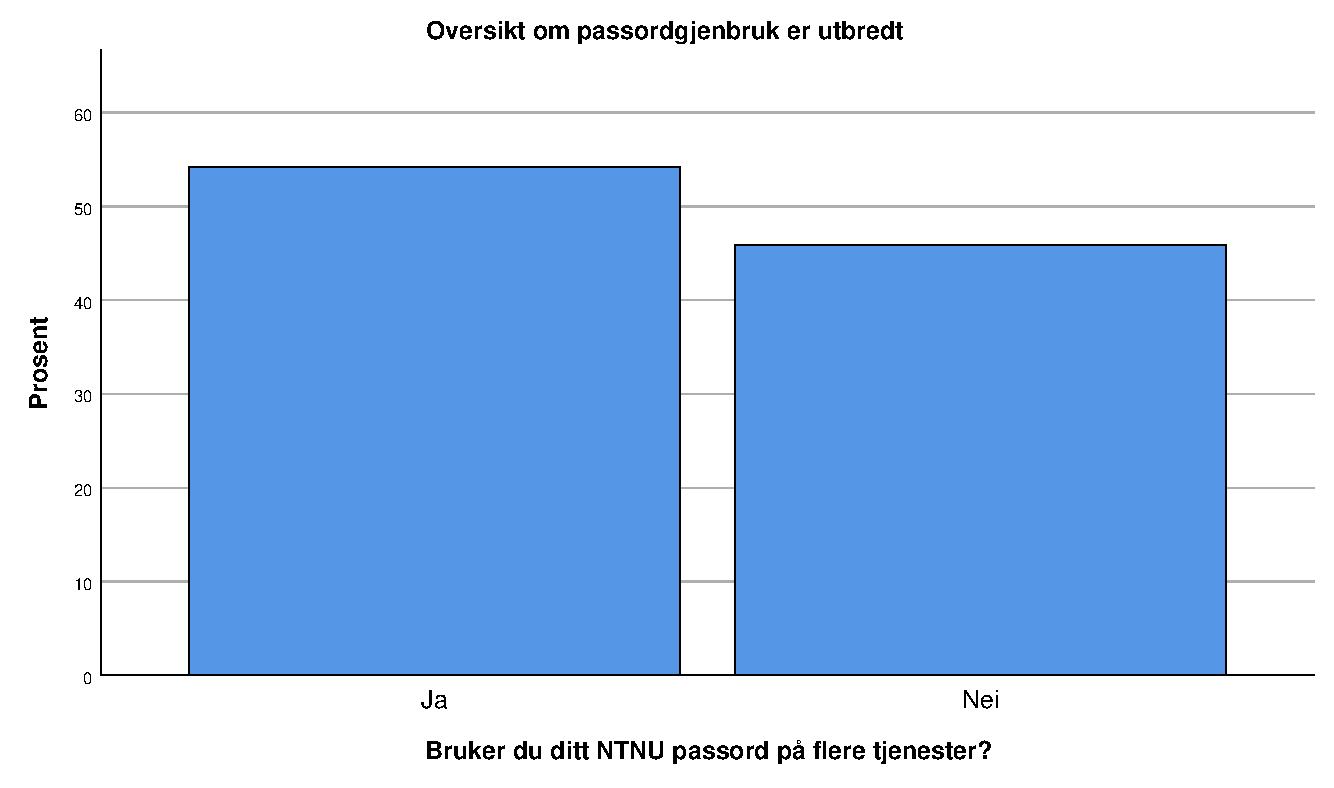
\includegraphics[scale=0.5]{case_2/bilder/spss/passordgjenbruk.pdf}
    \caption[Frekvens av passordgjenbruk]{Oversikt over gjenbruk av NTNU passord}
    \label{fig:case2-passordgjenbruk}
\end{figure}

Over 80\% av respondentene svarte at de ikke brukte regler når de lager passord.
\begin{figure}[H]
    \centering
    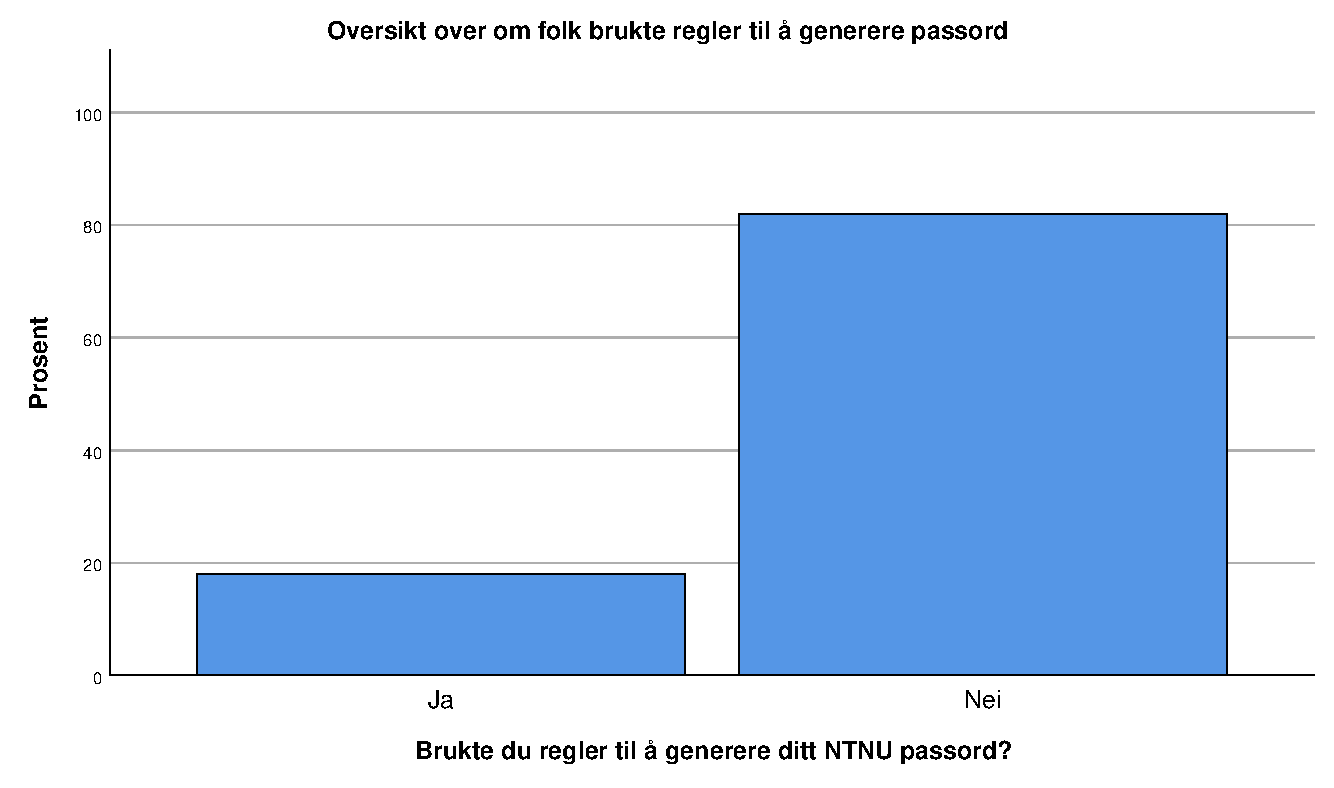
\includegraphics[scale=0.5]{case_2/bilder/spss/regler_passord.pdf}
    \caption[Bruk av passordregler]{Viser hvor mange som bruker passordregler}
    \label{fig:case2-passordregler}
\end{figure}

Over 80\% av respondentene har passord som er mellom 8-11 tegn. Resterende fordelte seg likt utover de andre valgene. 
\begin{figure}[H]
    \centering
    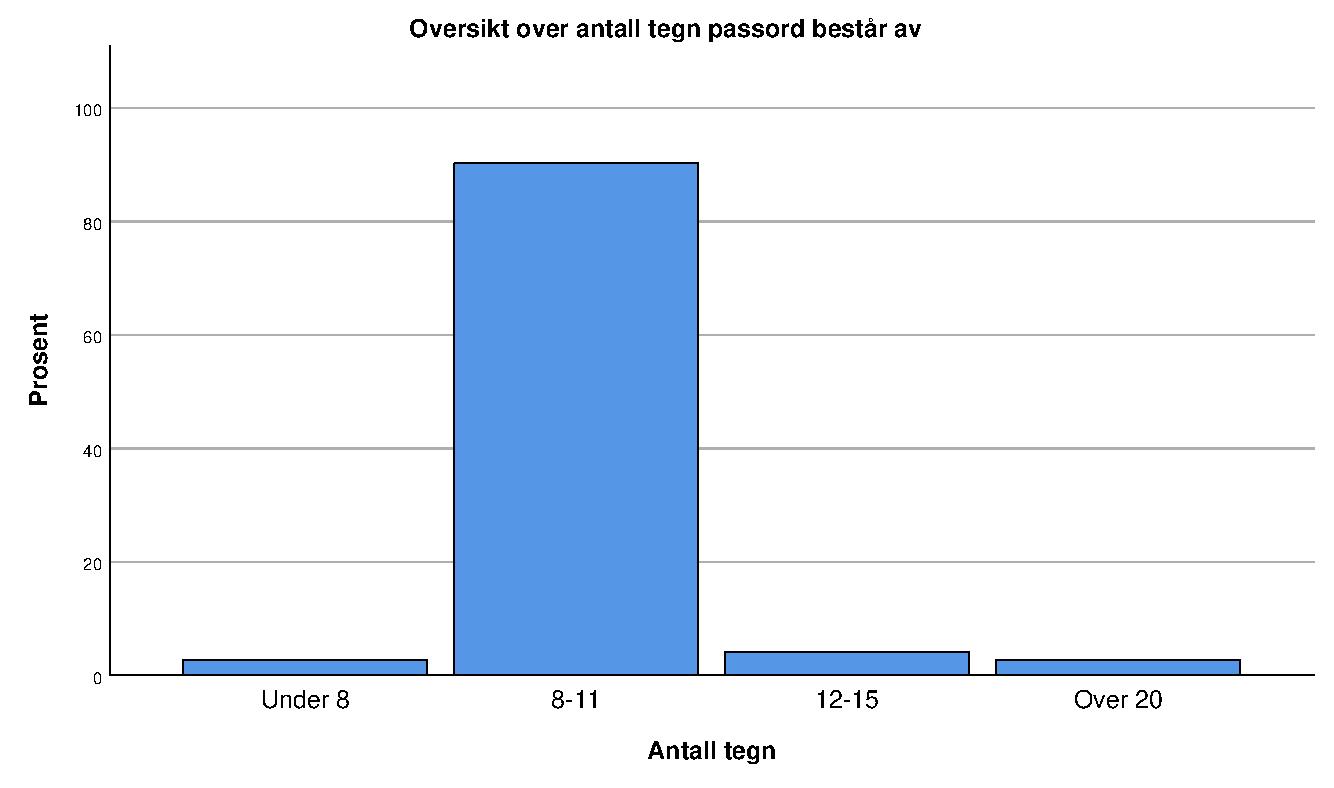
\includegraphics[scale=0.5]{case_2/bilder/spss/antall_tegn.pdf}
    \caption[Antall tegn i passord]{Antall tegn på passord}
    \label{fig:case2-antalltegn}
\end{figure}
Hypotesen vår var korrekt, de fleste bruker passord som er under 12 tegn. Det er mulig vi burde ha splittet opp intervallene ytterligere jo mindre antall tegn det var snakk om. 

Figur \ref{fig:case2-bytter-passord} viser statistikken over hvor ofte respondentene bytter passord. Over 50\% sier at de bytter passord sjeldnere enn hvert andre år, over 20\% sier at de bytter hvert andre år, rett under 20\% sier at de bytter hvert år og resten sier at de bytter hver sjette måned. 
\begin{figure}[H]
    \centering
    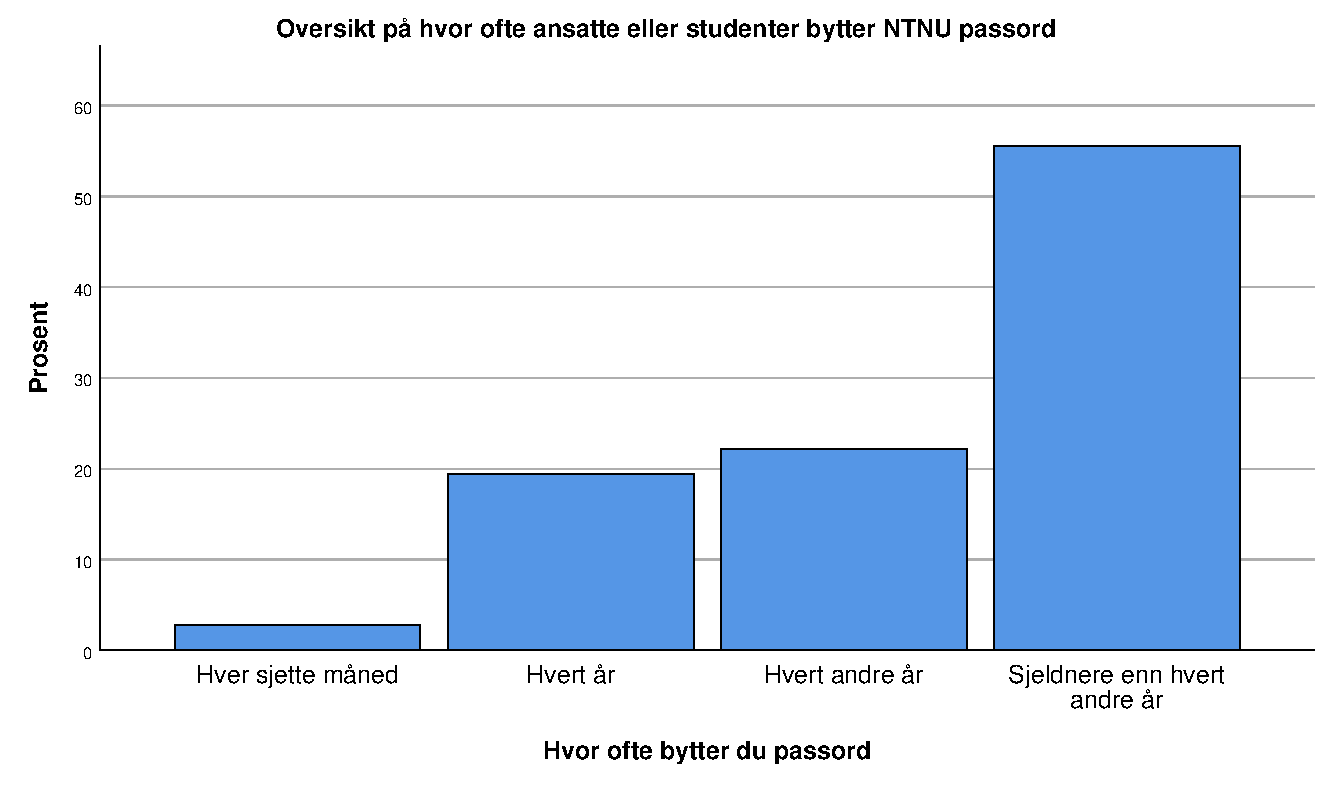
\includegraphics[scale=0.5]{case_2/bilder/spss/bytter_passord.pdf}
    \caption[Hvor ofte de bytter passord]{Viser hvor ofte de bytter passord}
    \label{fig:case2-bytter-passord}
\end{figure}
Hypotesen var korrekt, flertallet av respondentene bytter passord sjeldnere enn hvert andre år. I henhold til retningslinjer for passord, brukernavn og authentiseringsdata så skal passord byttes hver sjette måned og tvungen passordbytte hvert år. Dette viser at respondentene ikke kjent med IT-reglementet og reglementet blir ikke overholdt.

I figur \ref{fig:case2-passordsikkerhet} ser vi antallet som sier at de har fått opplæring i passordsikkerhet fra NTNU. Ut fra tabellen ser vi at under 80\% av respondentene sier at de ikke har fått opplæring i passordsikkerhet. 15\% sier at de ikke vet om de har fått opplæring og resten sier at de har fått det. 
\begin{figure}[H]
    \centering
    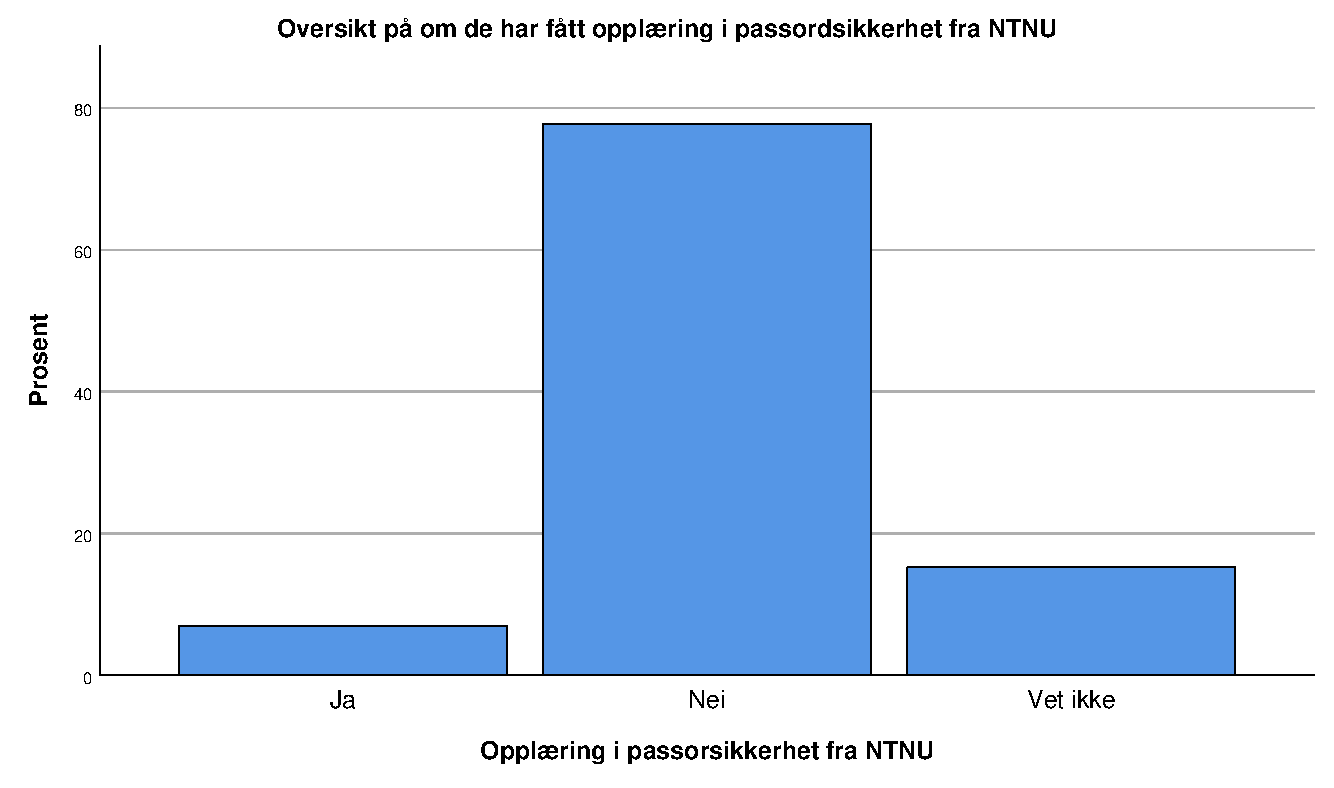
\includegraphics[scale=0.5]{case_2/bilder/spss/opplaring_passordsikk_NTNU.pdf}
    \caption[Opplæring i passordsikkerhet]{Viser hvor mange som har fått opplæring i passordsikkerhet}
    \label{fig:case2-passordsikkerhet}
\end{figure}

\subsection{Phishing}
Over 70\% av respondentene sa at de har oppdaget phishing e-post en eller flere ganger på sin NTNU e-post, og rett under 20\% som ikke har oppdaget phishing e-post. Resten av respondentene svarte at de ikke vet. Dette vises i figur \ref{fig:case2-oppdaget-phishing} under.
\begin{figure}[H]
    \centering
    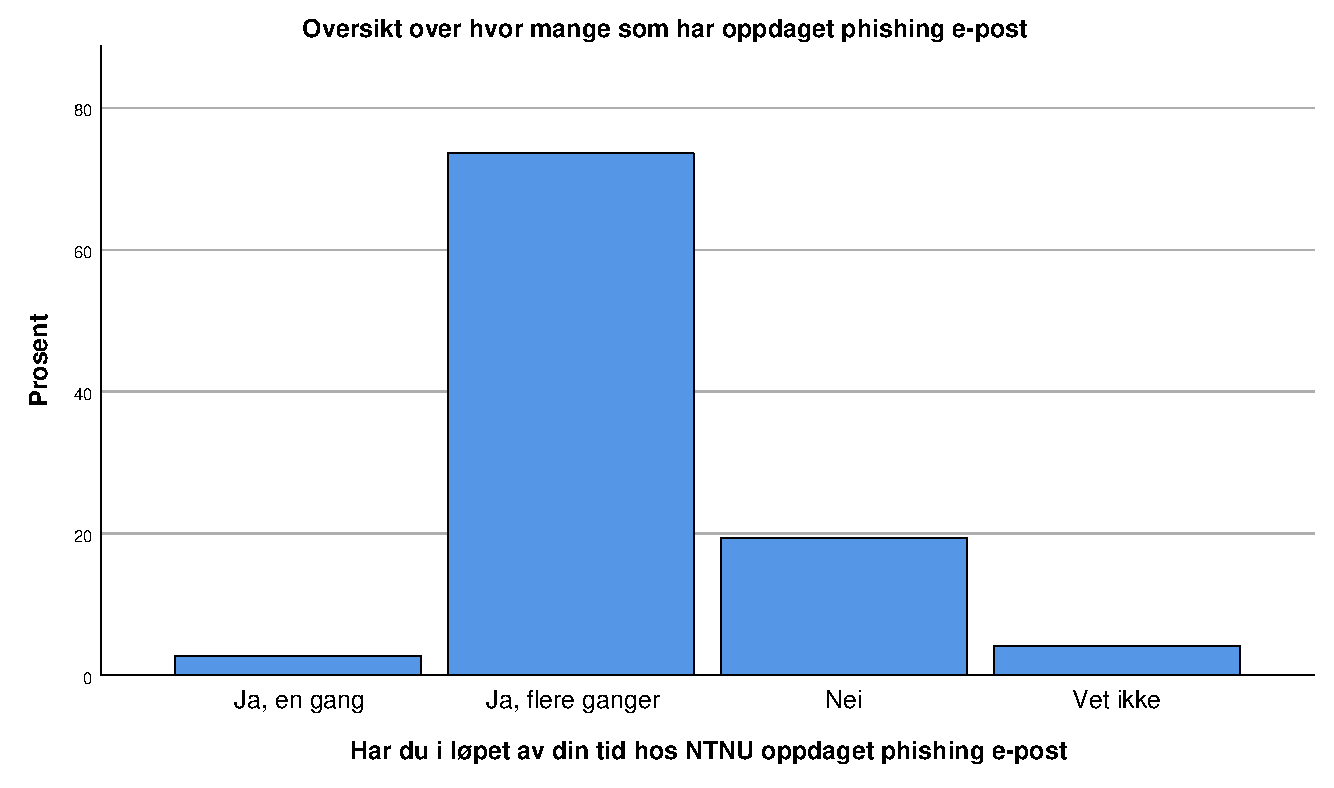
\includegraphics[scale=0.5]{case_2/bilder/spss/oppdaget_phish.pdf}
    \caption[Oppdaget phishing]{Viser hvor mange som har oppdaget phishing e-post}
    \label{fig:case2-oppdaget-phishing}
\end{figure}

Over 70\% av respondentene sier at de ikke har blitt lurt av phishing e-post, og under 20\% sier at de har blitt lurt. Som vist i tabellen under. 
\begin{figure}[H]
    \centering
    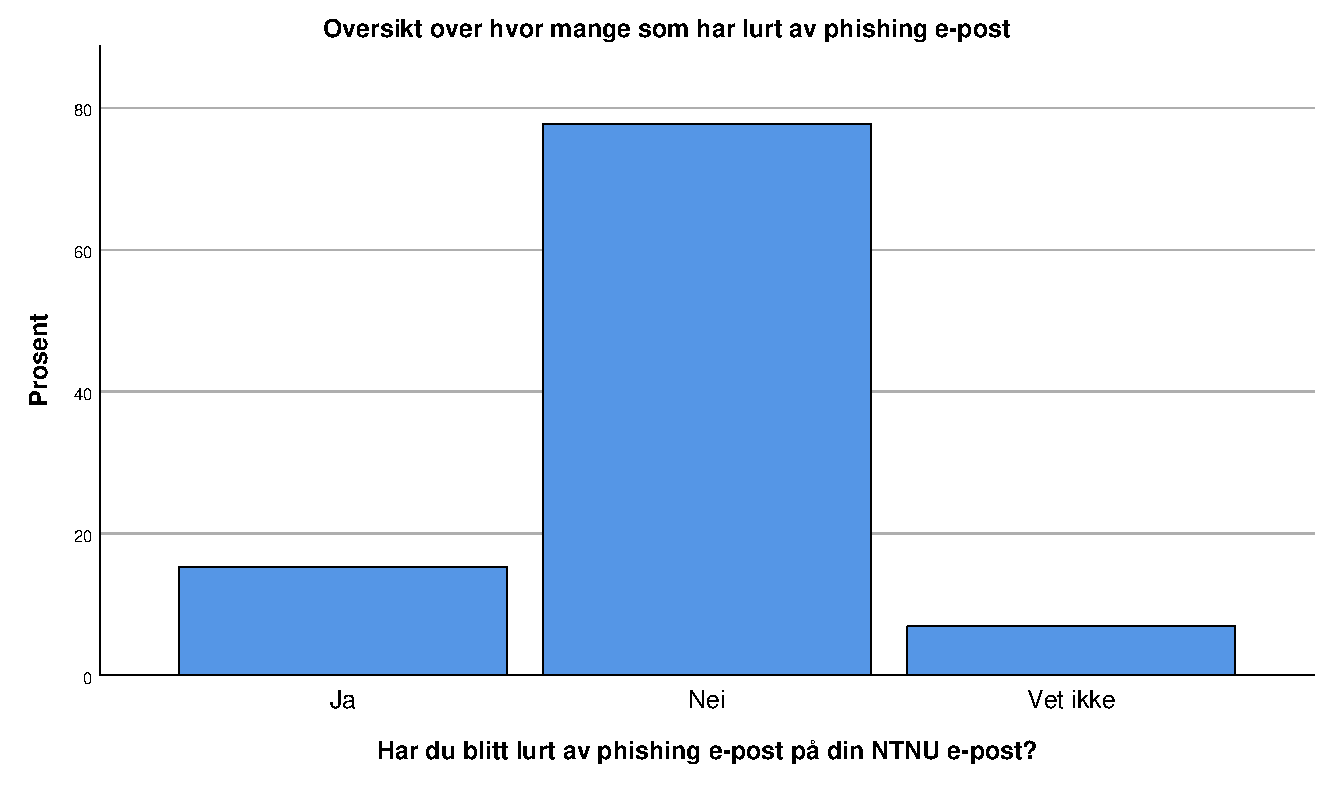
\includegraphics[scale=0.5]{case_2/bilder/spss/lurt_phish.pdf}
    \caption[Lurt av phishing]{Viser hvor mange som sier de har blitt lurt av phishing}
    \label{fig:lurt-av-phishing}
\end{figure}

\subsection{Statistisk analyse}
I denne delen bruker vi statistiske analyseverktøy for å finne relasjoner. De mindre relevante analysene er plassert i vedlegg \ref{vedlegg:statanalys}. Som en generell regel for utføring av analysen har vi valgt et signifikansnivå på: \[\alpha \leq 0,05\]

\subsubsection{ANOVA på alder mot bevissthet og kjennskap}
Denne testen sjekker om det er signifikans mellom alder på respondenten, og hvor bevisste de er på sikkerhet og hvor godt de kjenner til de ulike retningslinjene og reglementene. Alle spørsmålene er besvart på en skala fra 1 til 6, der 1 er lite bevisst eller kjent, og 6 er svært bevisst eller kjent. I tabellen under beskrives svarene til datasettet som er analysert. 
\begin{figure}[H]
    \centering
    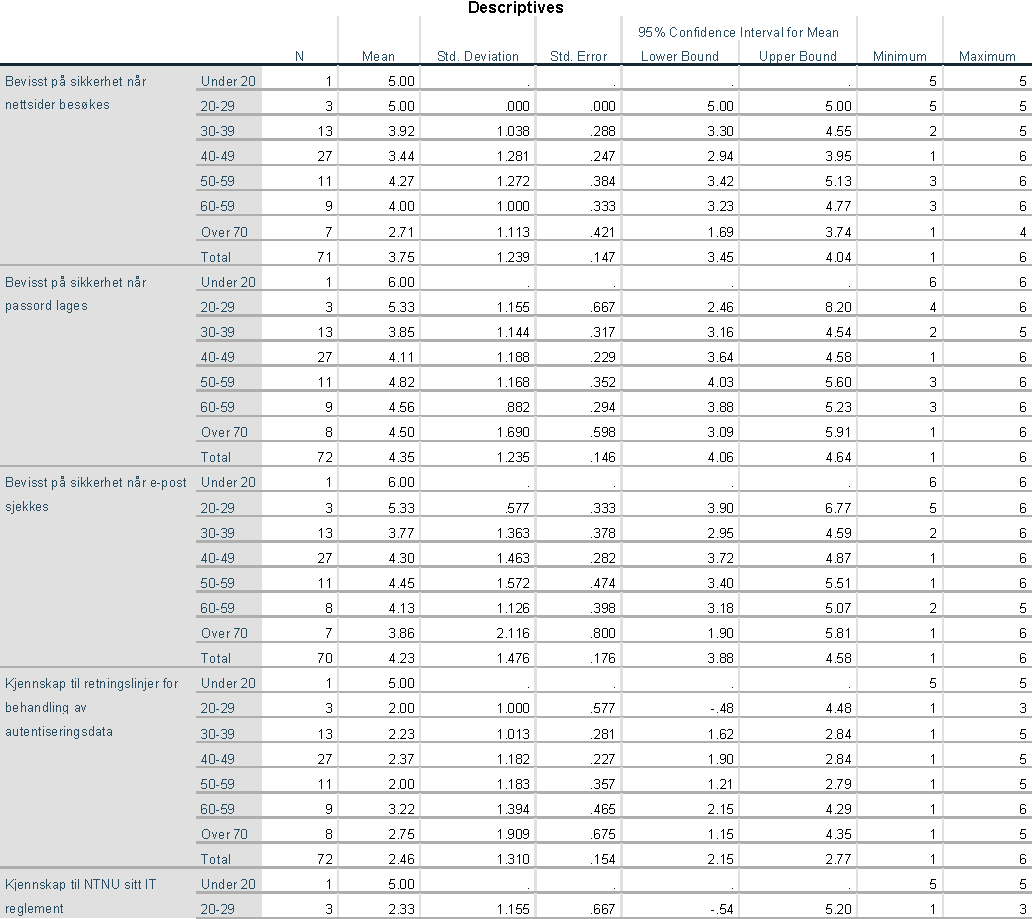
\includegraphics[scale=0.7]{case_2/bilder/spss/anova_ttest/alder_bevissthetogkjennskap_descriptive_1.pdf}
    \caption[Descriptive av alder mot bevissthet på sikkerhet og kjennskap til dokumenter del 1]{Descriptive av alder mot bevissthet på sikkerhet og kjennskap til retningslinjer, del 1}
    \label{fig:alder-bevissthetogkjennskap-descriptive-1}
\end{figure}

\begin{figure}[H]
    \centering
    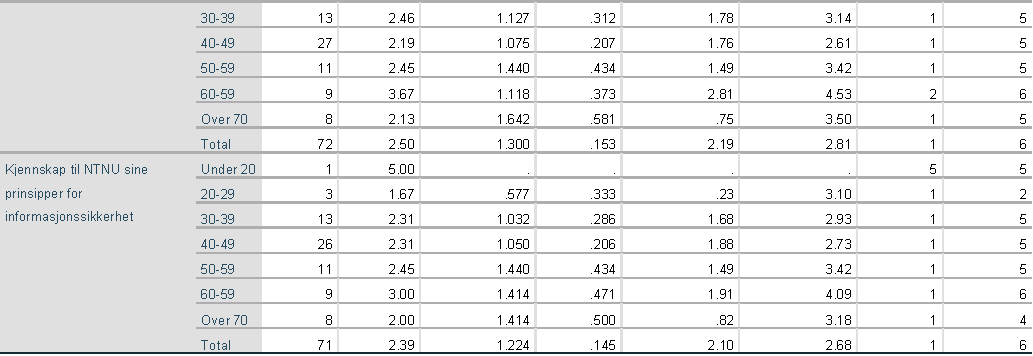
\includegraphics[scale=0.7]{case_2/bilder/spss/anova_ttest/alder_bevissthetogkjennskap_descriptive_2.pdf}
    \caption[Descriptive av alder mot bevissthet på sikkerhet og kjennskap til dokumenter del 1]{Descriptive av alder mot bevissthet på sikkerhet og kjennskap til retningslinjer, del 2}
    \label{fig:alder-bevissthetogkjennskap-descriptive-2}
\end{figure}

Fra dataene over kan vi se at generelt sett går bevisstheten på sikkerhet og kjennskapen til retningslinjene ned etterhvert som respondentene blir eldre. Dette gjelder spesielt for bevissthet på sikkerhet når nettsider besøkes og kjennskap til IT-reglementet. 

\begin{figure}[H]
    \centering
    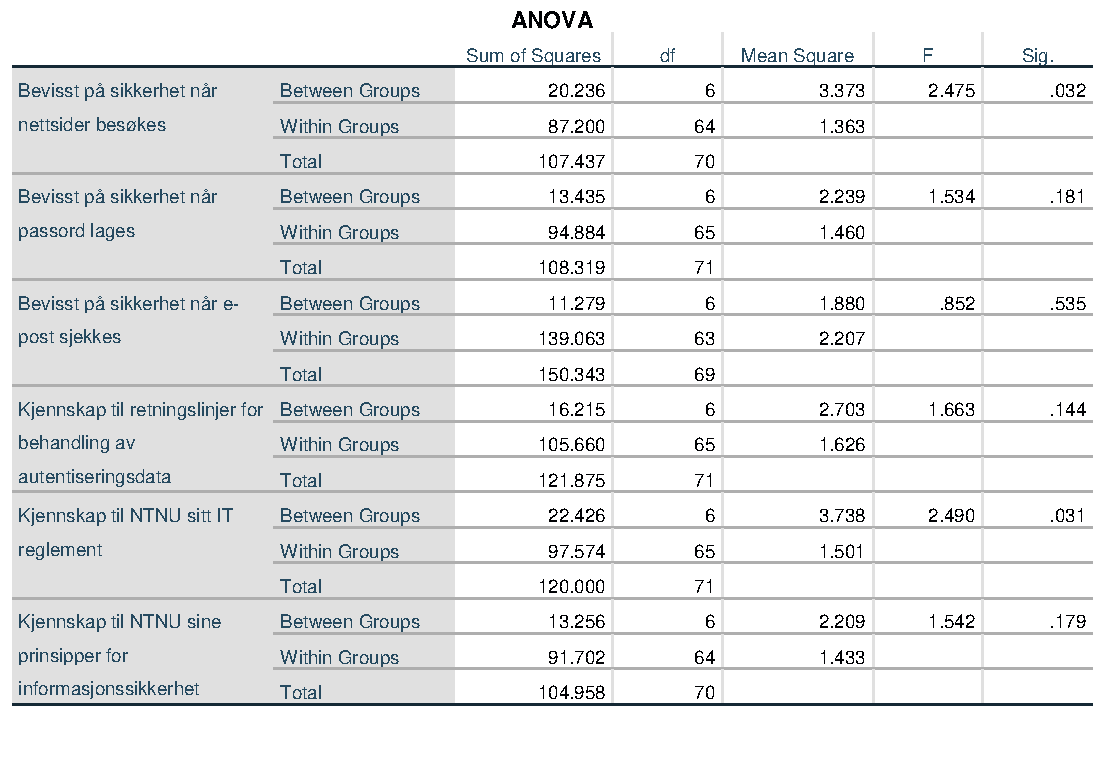
\includegraphics[scale=0.7]{case_2/bilder/spss/anova_ttest/alder_bevissthetogkjennskap_anova.pdf}
    \caption[ANOVA av alder mot bevissthet på sikkerhet og kjennskap til retningslinjer]{ANOVA av alder mot bevissthet på sikkerhet og kjennskap til dokumenter}
    \label{fig:alder-bevissthetogkjennskap-ANOVA}
\end{figure}

I tabellen over ser vi at når det kommer til alder basert på bevissthet på sikkerhet når nettsider besøkes er dette signifikant siden \(\alpha = 0,032\). Dette betyr at vi kan konkludere med at jo eldre folk blir, jo mindre bevisste er de på sikkerhet når de besøker nettsider. Dette gjelder også for kjennskap til NTNU sitt IT-reglement, der signifikansen er på \(\alpha = 0,031\). 

En post-hoc test kunne ikke kjøres her fordi en av kategoriene bare hadde ett svar. 

\subsubsection{ANOVA på år ved NTNU mot passord-, e-post- og andre brukervaner}
Denne testen sjekker om det er signifikans mellom antall år respondenten har vært hos NTNU, og om de bruker NTNU e-posten sin på andre tjenester, om de har blitt lurt av phishing og om de benytter sitt NTNU passord på flere tjenester. I tabellen under beskrives svarene til datasettet vi skal analysere.
\begin{figure}[H]
    \centering
    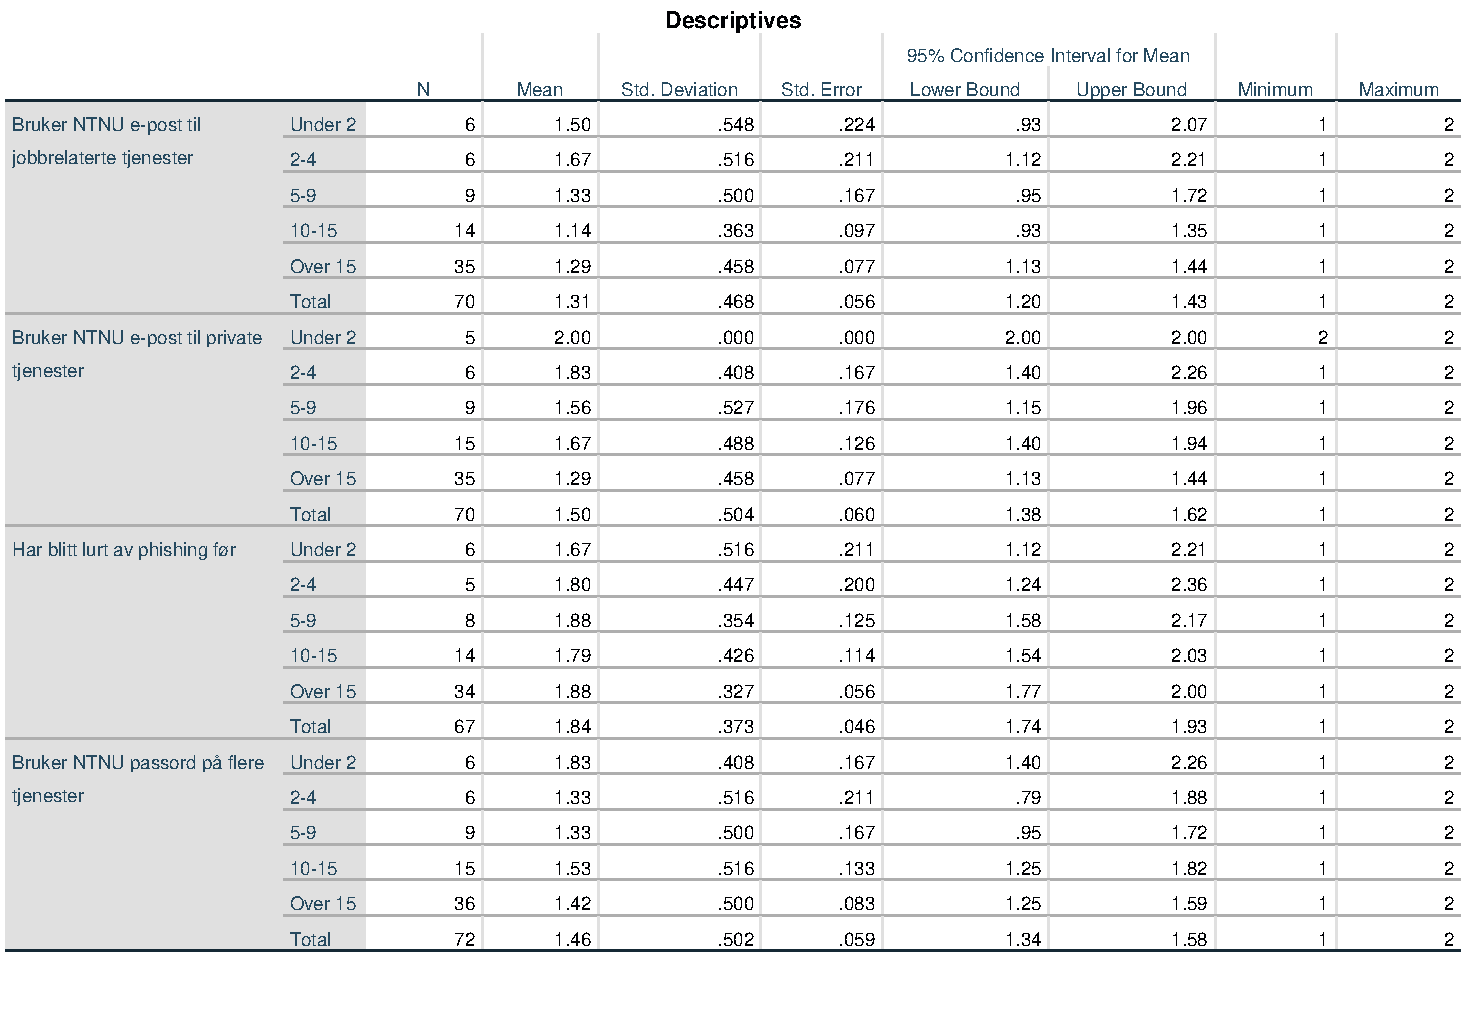
\includegraphics[scale=0.5]{case_2/bilder/spss/anova_ttest/ansiennitet_diverse_descriptive.pdf}
    \caption[Descriptive av år ved NTNU mot passord-, e-post- og andre brukervaner]{Descriptive av år ved NTNU mot passord-, e-post- og andre brukervaner}
    \label{fig:ansiennitet-diverse-descriptive}
\end{figure}

\begin{figure}[H]
    \centering
    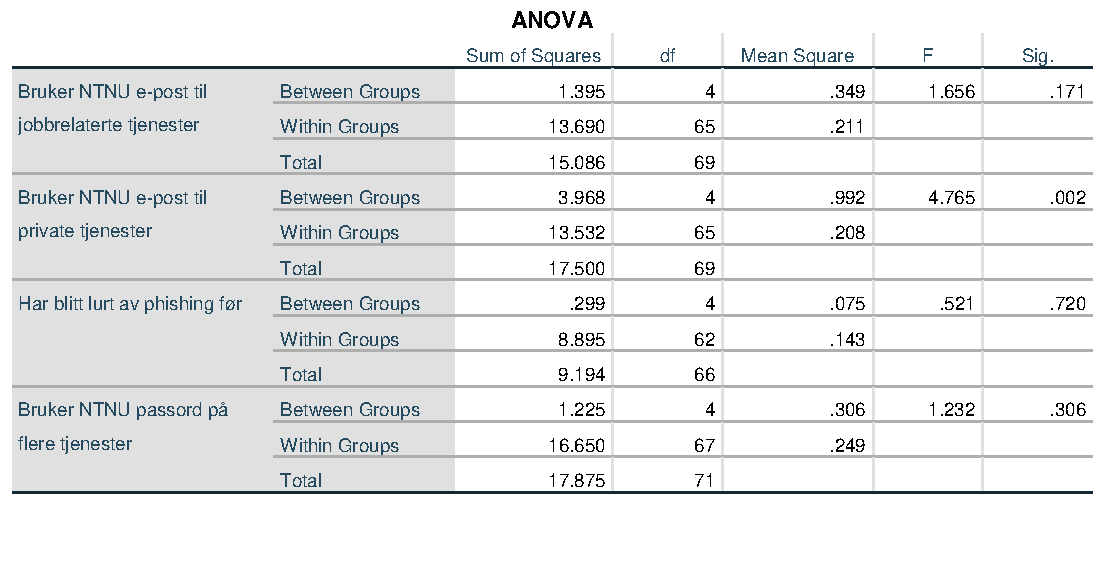
\includegraphics[scale=0.7]{case_2/bilder/spss/anova_ttest/ansiennitet_diverse_anova.pdf}
    \caption[ANOVA av år ved NTNU mot passord-, e-post- og andre brukervaner]{ANOVA av år ved NTNU mot passord-, e-post- og andre brukervaner}
    \label{fig:ansiennitet-diverse-ANOVA}
\end{figure}

Siden det er signifikans på de som bruker NTNU e-post til private tjenester (\(\alpha \leq 0,05\)), ble en post-hoc test kjørt for å se om det var noen ytterligere signifikans mellom gruppene. Grunnet plassbesparelse er bare de variablene som inkluderte signifikans tatt med i rapporten. 

\begin{figure}[H]
    \centering
    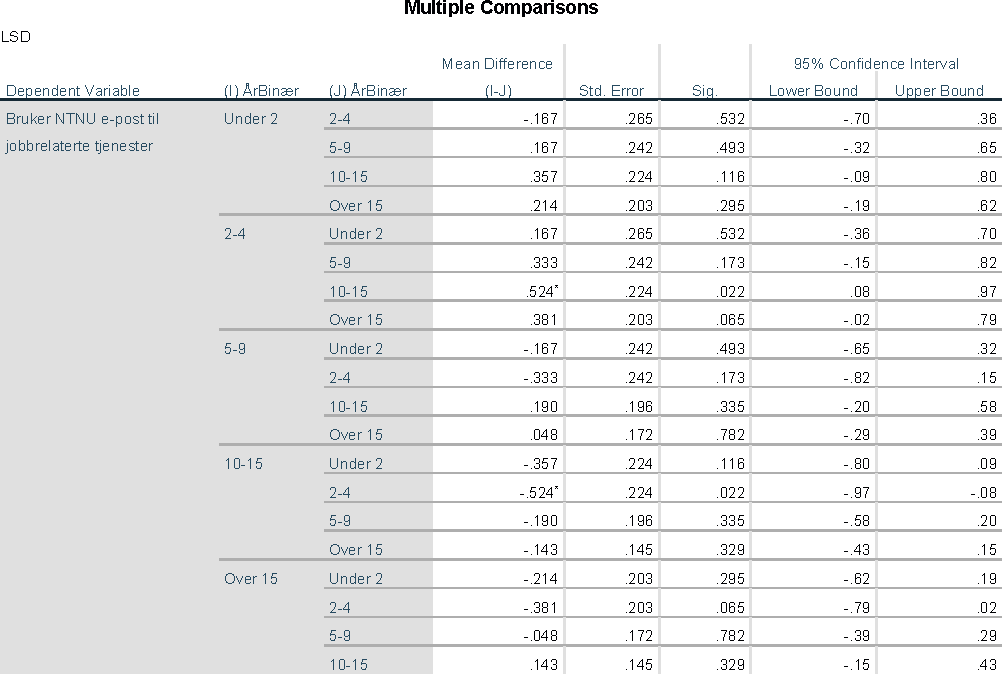
\includegraphics[scale=0.7]{case_2/bilder/spss/anova_ttest/ansiennitet_diverse_posthoc_1.pdf}
    \caption[Post-hoc av år ved NTNU mot passord-, e-post- og andre brukervaner del 1]{Post-hoc av år ved NTNU mot passord-, e-post- og andre brukervaner, del 1}
    \label{fig:alder-bevissthetogkjennskap-posthoc-1}
\end{figure}

\begin{figure}[H]
    \centering
    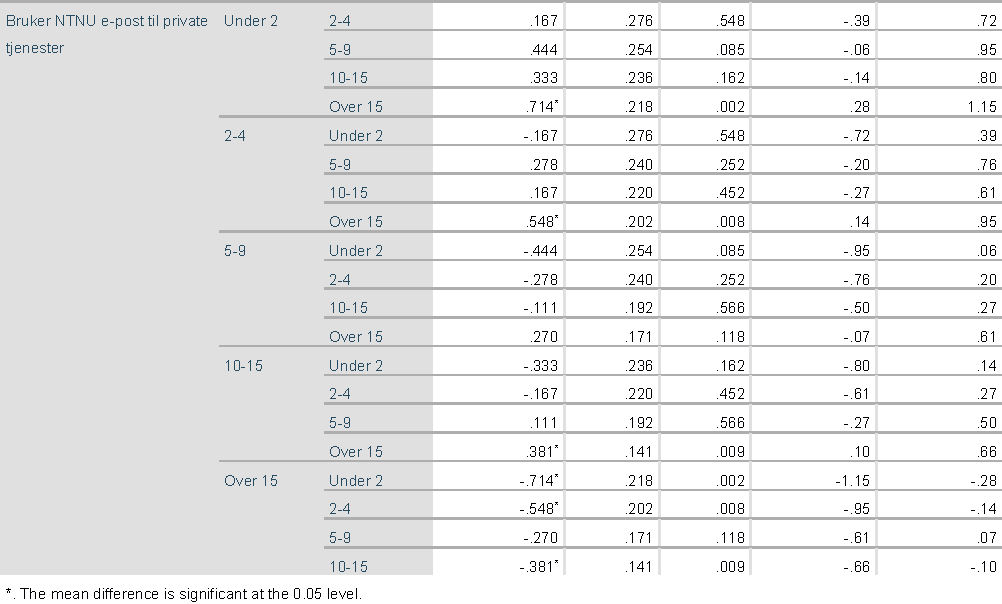
\includegraphics[scale=0.7]{case_2/bilder/spss/anova_ttest/ansiennitet_diverse_posthoc_2.pdf}
    \caption[Post-hoc av år ved NTNU mot passord-, e-post- og andre brukervaner del 2]{Post-hoc av år ved NTNU mot passord-, e-post- og andre brukervaner, del 2}
    \label{fig:alder-bevissthetogkjennskap-posthoc-2}
\end{figure}

I post-hoc testen i figur \ref{fig:alder-bevissthetogkjennskap-posthoc-1} og \ref{fig:alder-bevissthetogkjennskap-posthoc-2} ser vi at når det kommer til jobbrelaterte tjenester er forskjellen signifikant mellom de som har vært ved NTNU i 2-4 år og 10-15 år. Når det kommer til private tjenester er forskjellen signifikant mellom under 2 år og over 15, 2-4 år og over 15, og mellom 10-15 år og over 15. Vi ser at det er en relasjon mellom hvor mange år ved NTNU de og om de bruker NTNU e-post på andre tjenester. Jo lenger de er der, jo mer sannsynlig er det at de bruker e-posten på flere tjenester. 

\subsubsection{ANOVA på alder mot passord-, e-post- og andre brukervaner}
Siden det ble funnet signifikans på antall år ved NTNU og bruk av NTNU e-post på private tjenester, kunne det være sannsynlig at dette også korrelerte med alder. Det er logisk å tro at jo lenger tid en har tilbringet ved NTNU, jo eldre er personen. Derfor ble det kjørt en korrelasjonstest på alder og antall år ved NTNU for å teste dette. I tabellen under kan vi se at det er en sterk positiv korrelasjon (\(\alpha \le 0,01\)) mellom alder og tid ved NTNU.

\begin{figure}[H]
    \centering
    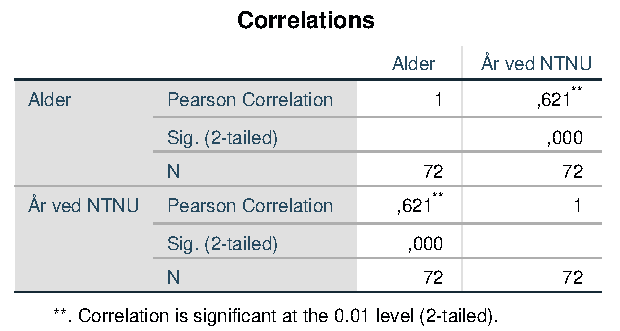
\includegraphics[scale=1]{case_2/bilder/spss/anova_ttest/alder_aarvedNTNU_korrelasjon.pdf}
    \caption[Korrelasjon mellom alder og antall år ved NTNU]{Korrelasjon mellom alder og antall år ved NTNU}
    \label{fig:alder-aarvedNTNU-korrelasjon}
\end{figure}

Basert på resultatene er det grunnlag for å tro at siden jo eldre respondenten som har fått sin konto kompromittert er, jo mer sannsynlig er det at personen har benyttet e-posten på private tjenester, basert på resultatene i figur \ref{fig:ansiennitet-diverse-ANOVA} i forrige seksjon.

\subsection{Independent sample t-test på de som har delt passord mot hvor ofte de bytter passord}
Selv om det bare er åtte personer som har sagt at de har delt sitt NTNU passord er dette åtte personer for mye. I IT-reglementet står det at dersom du har mistanke om at noen kan passordet, skal du bytte det med en gang \cite{ITReg}. Derfor var det relevant å se hvor ofte de som har delt passordet sitt bytter passord. Variabelen ``ByttePassordBinær'' går fra 1-4 der 1 er bytte av passord hver sjette måned og 4 er hvert andre år. 

\begin{figure}[H]
    \centering
    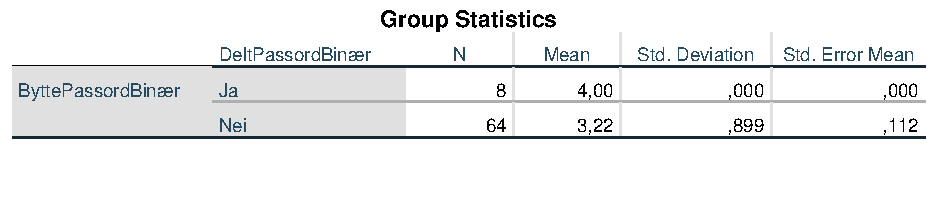
\includegraphics[scale=0.7]{case_2/bilder/spss/anova_ttest/deltpassord_byttepassord_groupstats.pdf}
    \caption[Group statistics av de som har delt passord mot hvor ofte de bytter]{Group statistics av de som har delt passord mot hvor ofte de bytter}
    \label{fig:deltpassord-byttepassord-groupstats}
\end{figure}

Statistikken i figur \ref{fig:deltpassord-byttepassord-groupstats} over viser at alle de som har delt passordet sitt, bytter passord sjeldnere enn hvert andre år. Dette er bekymringsfullt i og med at passordene er kjent av andre over lengre tid. I figur \ref{fig:deltpassord-byttepassord-ttest} sjekker vi om disse tallene er signifikante.

\begin{figure}[H]
    \centering
    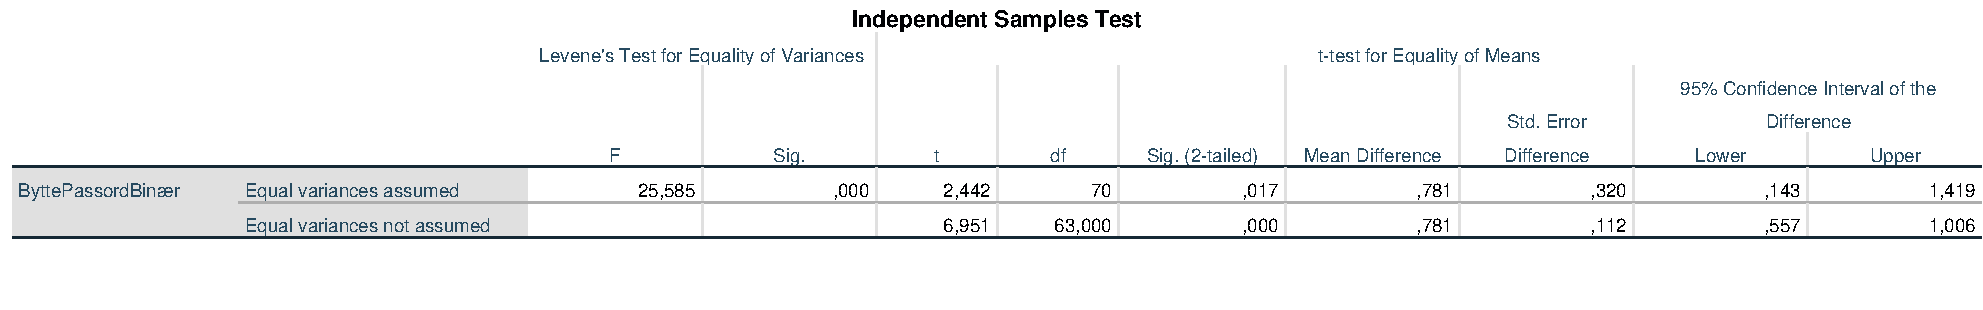
\includegraphics[scale=0.4]{case_2/bilder/spss/anova_ttest/deltpassord_byttepassord_ttest.pdf}
    \caption[Independent t-test av de som har delt passord mot hvor ofte de bytter]{Independent t-test av de som har delt passord mot hvor ofte de bytter}
    \label{fig:deltpassord-byttepassord-ttest}
\end{figure}

Vi kan se at \(\alpha = 0,017\), som betyr at resultatet er statistisk signifikant. 


\section{Rotårsaksidentifisering}

\subsection{Årsak-virkningsdiagram}
Innledningsvis ble problemet beskrevet som rotårsaken til kompromitterte kontoer ved NTNU. Hovedkategoriene som ble undersøkt for å finne svar på dette var gjenbruk av innloggingskredentialier tilhørende NTNU, IT-reglementet og andre styringsdokumenter, passordvaner, phishing og oversikt over situasjonen. Både hovedkategoriene og årsakene under disse er i hovedsak basert på dataanalysen, mens noe er basert på kreativ idémyldring. 

\begin{figure}[H]
    \centering
    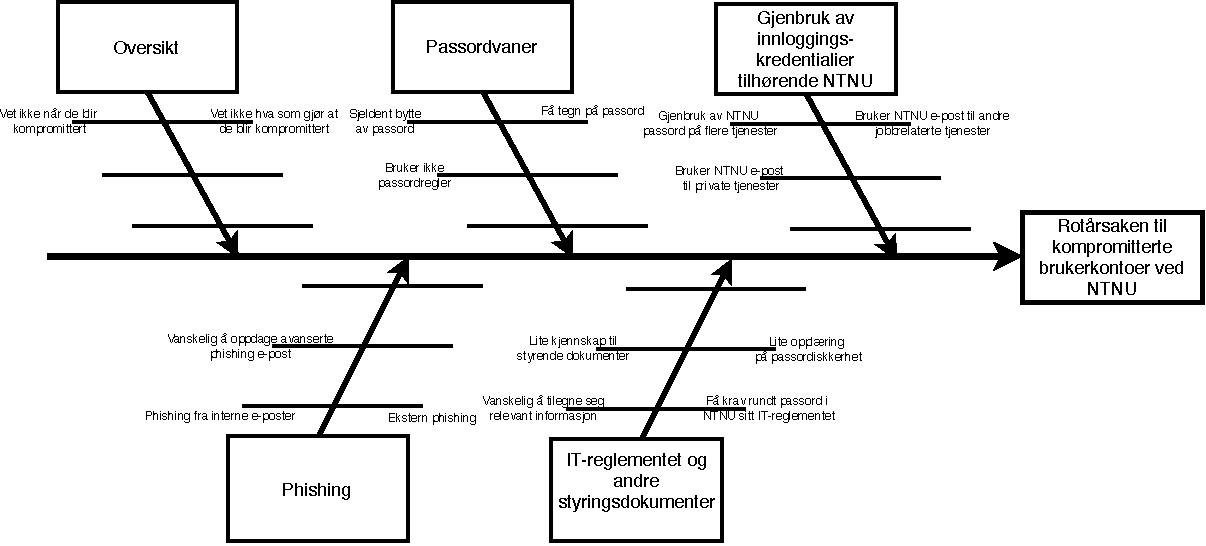
\includegraphics[scale=0.65]{case_2/bilder/fiskebein.pdf}
    \label{fig:fiskebein-case2}
    \caption[Fiskebeindiagram for kompromitterte kontoer]{Fiskebeindiagram over hovedkategorier og årsaker til kompromitterte kontoer}
\end{figure}

Vi har kommet frem til at rotårsaken til kompromitterte kontoer er sammensatt av flere faktorer. Et passord på mellom åtte til elleve tegn i seg selv er ikke nok for at kontoen skal bli kompromittert, men sammen med at de bytter sjeldnere enn hvert andre år gjør at dette blir et problem. I tillegg til dette bruker flertallet NTNU e-posten til andre tjenester, enten til jobbrelatert eller til privat bruk. De bruker også samme NTNU passord på flere tjenester. Dette er noe en burde unngå til enhver tid, og er noe av det vi anser å være blant det mest kritiske. 

Respondentene hadde også liten kjennskap til IT-reglementet og andre styringsdokumenter. De svarte også at de har fått lite opplæring på passordsikkerhet. Vi har lest gjennom IT-reglementet og andre styringsdokumenter, og har kommet frem til at IT-reglementet har for få krav til passord. Det var vanskelig å tilegne seg all informasjon på de forskjellige styringsdokumentene da IT-reglementet ikke henviste til noen av retningslinjene. I retningslinjer for behandling av brukernavn, passord og andre autentiseringsdata \cite{RetnBPA} står det at passordet skal byttes hver 12 måned. Denne retningslinjen er ikke nevnt i IT-reglementet at du skal gjøre deg bekjent med. 

Sammenlagt så viste det oss at respondentene hadde dårlige passordvaner, gjenbruk av innloggingskredentialier tilhørende NTNU og lite kunnskap til IT-reglementet og andre styrende dokumenter. Phishing er også en relevant årsak til kompromitterte kontoer. Phishing e-poster har blitt såpass sofistikerte at det er vanskelig å skille mellom falske og legimite e-poster. \cite{SophPhish}. Rotårsakene er derfor som følger: 

\begin{itemize}
    \item Mistet kontodetaljer av phishing
    \item E-post og passordgjenbruk på andre tjenester
    \item Liten kjennskap til IT-reglement og andre styrende dokumenter
    \item Dårlige passordvaner
\end{itemize}

\subsection{5 Whys}
Det ble fremhevet fem årsaker som skulle analyseres. Fire av disse kom fra fiskebeindiagrammet over, og en fra idémyldring. Tabellene under viser resultatene fra gjennomføringen. 

\begin{table} [H]
    \centering
    \begin{tabular}{ | m{5em} | m{30em} | }
        \hline
            \cellcolor{yellow} Årsak: & \cellcolor{yellow} Mistet kontodetaljer av phishing                \\
        \hline
            Why? & Fordi e-posten kom fra en intern e-postadresse                                   \\
        \hline
            Why? & Fordi kontoen var blitt kompomittert                                             \\
        \hline
            Why? & Fordi kontodetaljene ble phishet fra en ekstern e-postadresse                \\
        \hline
            Why? & Fordi brukeren var ikke oppmerksom på at det var en phishing e-post              \\
        \hline
            Why? & Fordi brukeren hadde ikke fått tilstrekkelig opplæring i deteksjon av phishing e-post    \\
        \hline
    \end{tabular}
    \caption[5 Whys: Mistet kontodetaljer av phishing]{5 Whys på mistet kontodetaljer av phishing}
    \label{5Whys-phishing}
\end{table}

Å miste kontodetaljer av en phishing e-post kan skje fra enten interne eller eksterne e-postadresser. I 5 Whys over kom vi frem til at dette skjer fordi en ikke er oppmerksom på tvilsomme e-poster. Årsaken til det kan være fordi brukerne ikke har fått tilstrekkelig opplæring i deteksjon av phishing e-post.

\begin{table} [H]
    \centering
    \begin{tabular}{ | m{5em} | m{30em} | }
        \hline
            \cellcolor{yellow} Årsak: & \cellcolor{yellow} E-post og passordgjenbruk på andre tjenester \\
        \hline
            Why? & Fordi det er vanskelig å huske mange unike brukerdetaljer \\
        \hline
            Why? & Fordi det ikke brukes passordmanager \\
        \hline
            Why? & Fordi de ikke vet hva det er \\
        \hline
            Why? & Fordi det ikke gis informasjon om det i retningslinjene \\
        \hline
            Why? & - \\
        \hline
    \end{tabular}
    \caption[5 Whys: E-post og passordgjenbruk på andre tjenester]{5 Whys på e-post og passordgjenbruk på andre tjenester}
    \label{5Whys-phishing}
\end{table}

Årsaken til at mange velger å benytte samme kredentialer flere steder er som regel at de synes det er vanskelig å huske mange brukerdetaljer, og motsatt, enkelt å huske få. Noe som kan gjøre dette lettere er å bruke en passordmanager, men dette informeres det ikke om i styringsdokumentene. 

\begin{table} [H]
    \centering
    \begin{tabular}{ | m{5em} | m{30em} | }
        \hline
            \cellcolor{yellow} Årsak: & \cellcolor{yellow} Liten kjennskap til IT-reglement og andre styrende dokumenter \\
        \hline
            Why? & Fordi det er vanskelig å tilegne seg informasjon \\
        \hline
            Why? & Fordi informasjonen er spredt på mange sider og dokumenter \\
        \hline
            Why? & Fordi det ikke er et overordnet ISMS \\
        \hline
            Why? & - \\
        \hline
            Why? & - \\
        \hline
    \end{tabular}
    \caption[5 Whys: Liten kjennskap til IT-reglement og andre styrende dokumenter]{5 Whys på liten kjennskap til IT-reglement og andre styrende dokumenter}
    \label{5Whys-phishing}
\end{table}

En mulig årsak til at det er liten kjennskap til disse dokumentene er at det er vanskelig å tilegne seg informasjonen. Det blir ofte mye for en person å forholde seg til, spesielt når informasjonen er spredt utover mange forskjellige sider og dokumenter. Et overordnet ISMS kunne hjulpet med å standardisere sikkerhetsstyringen, og kanskje sentralisere informasjonen. 

\begin{table} [H]
    \centering
    \begin{tabular}{ | m{5em} | m{30em} | }
        \hline
            \cellcolor{yellow} Årsak: & \cellcolor{yellow} Dårlige passordvaner \\
        \hline
            Why? & Fordi de er lite bevisste på sikkerhet \\
        \hline
            Why? & Fordi de tenker det ikke er så viktig \\
        \hline
            Why? & Fordi det er ingen tydelige krav rundt passord i NTNU sitt IT-reglement \\
        \hline
            Why? & Fordi IT-reglementet ikke henviser til de relevante dokumentene \\
        \hline
            Why? & - \\
        \hline
    \end{tabular}
    \caption[5 Whys: Dårlige passordvaner]{5 Whys på dårlige passordvaner}
    \label{5Whys-passordvaner}
\end{table}

Mange har dårlige passordvaner, fordi de er lite bevisste på sikkerhet, og at de ikke tenker det er så viktig. Mulig årsak til dette kan være fordi det ikke er noen tydelige krav rundt passord i NTNU sitt IT-reglement. IT-reglementet henviser ikke til de dokumentene som nevner passordrutiner \cite{ITReg}, og det er bare IT-reglementet brukerne er pliktig å sette seg inn i og skrive under på \cite{}. 

\begin{table} [H]
    \centering
    \begin{tabular}{ | m{5em} | m{30em} | }
        \hline
            \cellcolor{yellow} Årsak: & \cellcolor{yellow} Lukrativt for trusselaktører \\
        \hline
            Why? & Fordi de tjener og sparer penger på å kompromittere kontoer \\
        \hline
            Why? & Fordi de får tilgang til forskningsdatabaser \\
        \hline
            Why? & Fordi det er for enkelt å få tilgang til brukerkontoene \\
        \hline
            Why? & Fordi det er utilstrekkelig tilgangskontroll på brukerkontoene \\
        \hline
            Why? & - \\
        \hline
    \end{tabular}
    \caption[5 Whys: Lukrativt for datakriminelle]{5 Whys på lukrativitet for datakriminelle}
    \label{5Whys-passordvaner}
\end{table}

Det er lukrativt for datakriminelle å prøve å kompromittere brukerkontoer fordi det er for god kost-nytte effekt. De kan tjene penger på å selge kontoene, eller spare penger ved å laste ned forskningsartikler. Her kom vi frem til at utilstrekkelig tilgangskontroll kan være en rotårsak til at det er så høy kost-nytteverdi for trusselaktørene.

\section{Rotårsakseliminering}

\subsection{Systematisk Innovativ Tenkning (SIT)}
Alle komponenter som eksisterer i problemets naturlige omgivelser listes under:

\begin{itemize}
    \item E-postadresse
    \item Brukernavn
    \item Autentisering
    \item IT-reglement
    \item Retningslinjer for behandling av brukernavn, passord og andre autentiseringsdata
    \item Prinsipper for informasjonssikkerhet (inkludert Policy)
    \item Påloggingssystem
    \item E-post filter
\end{itemize}

Når komponentene er gjort rede for, vil de fem SIT prinsippene brukes sekvensielt på komponentene for å utvikle løsninger på problemene. Ikke alle SIT-prinsipper finner løsninger som er gjennomførbare for alle komponenter. I disse tilfellene vil det stå: ``Ikke gjennomførbart''. Resultatene fremheves under.

\paragraph{E-post}
\begin{itemize}
    \item \textbf{Attributtavhengighet} Ikke gjennomførbart.
    \item \textbf{Komponentkontroll} Bevisstgjøringskampanje for god e-postskikk.
    \item \textbf{Erstatning} Gi folk kurs og hjelp til å ordne private e-postadresser.
    \item \textbf{Forkastning} Ikke gjennomførbart.
    \item \textbf{Oppdeling} Gi folk en egen epost adresse som bare skal brukes til privat bruk.
\end{itemize}

\paragraph{Brukernavn}
\begin{itemize}
    \item \textbf{Attributtavhengighet} Ikke gjennomførbart.
    \item \textbf{Komponentkontroll} Ikke gjennomførbart.
    \item \textbf{Erstatning} Ha mer tilfeldig brukernavn som er vanskeligere å gjette.
    \item \textbf{Forkastning} Ikke la e-postadressen kunne brukes som brukernavn.
    \item \textbf{Oppdeling} Ikke gjennomførbart.
\end{itemize}

\paragraph{Autentisering}
\begin{itemize}
    \item \textbf{Attributtavhengighet} Krav om sterkere passord.
    \item \textbf{Komponentkontroll} Bruke passordmanager for å behandle passord. 
    \item \textbf{Erstatning} Ikke gjennomførbart.
    \item \textbf{Forkastning} Ikke gjennomførbart.
    \item \textbf{Oppdeling} Gå over til 2-faktor autentisering.
\end{itemize}

\paragraph{IT-reglement}
\begin{itemize}
    \item \textbf{Attributtavhengighet} Utbedre IT-reglementet med tydeligere krav rundt passord. 
    \item \textbf{Komponentkontroll} Henvise til de andre styringsdokumentene.
    \item \textbf{Erstatning} Ikke gjennomførbart.
    \item \textbf{Forkastning} Ikke gjennomførbart.
    \item \textbf{Oppdeling} Ikke gjennomførbart.
\end{itemize}

\paragraph{Retningslinjer for behandling av brukernavn, passord og andre autentiseringsdata}
\begin{itemize}
    \item \textbf{Attributtavhengighet} Ikke gjennomførbart.
    \item \textbf{Komponentkontroll} Bevisstgjøringskampanje.
    \item \textbf{Erstatning} Legge retningslinjene inn i IT-reglementet.
    \item \textbf{Forkastning} Ikke gjennomførbart.
    \item \textbf{Oppdeling} Ikke gjennomførbart.
\end{itemize}

\paragraph{Prinsipper for informasjonssikkerhet}
\begin{itemize}
    \item \textbf{Attributtavhengighet} Ikke gjennomførbart.
    \item \textbf{Komponentkontroll} Integrere det i et ISMS
    \item \textbf{Erstatning} Ikke gjennomførbart.
    \item \textbf{Forkastning} Ikke gjennomførbart.
    \item \textbf{Oppdeling} Ikke gjennomførbart.
\end{itemize}

\paragraph{Påloggingssystem}
\begin{itemize}
    \item \textbf{Attributtavhengighet} Øk minimum antall tegn på passord fra 8 til 10. 
    \item \textbf{Komponentkontroll} Overholde kravet om å bytte passord hver 12. måned.
    \item \textbf{Erstatning} Ikke gjennomførbart. 
    \item \textbf{Forkastning} Ikke gjennomførbart. 
    \item \textbf{Oppdeling} Enhetskontroll på nye innlogginger.
\end{itemize}

\paragraph{E-post filter}
\begin{itemize}
    \item \textbf{Attributtavhengighet} Forbedre e-post filter.
    \item \textbf{Komponentkontroll} Ikke gjennomførbart. 
    \item \textbf{Erstatning} Ikke gjennomførbart. 
    \item \textbf{Forkastning} Ikke gjennomførbart. 
    \item \textbf{Oppdeling} Ikke gjennomførbart. 
\end{itemize}

Vi sorterer og beskriver de mest relevante idéer til videre utdyping:

\begin{description}
\item[Bevisstgjøringskampanje for god e-postskikk]
Med god e-postskikk så mener vi at brukerene er bevisste på om e-post er legitim eller ikke, og at NTNU e-post ikke skal bli benyttet til andre tjenester.

\item[Gi folk kurs og hjelp til å ordne private e-postadresser]
Det er et problem at folk bruker sin NTNU e-post til andre tjenester. Dette kan være fordi de ikke har en egen privat e-post de kan bruke til dette. Dette tiltaket vil hjelpe de med å anskaffe en privat e-post, så de ikke bruker NTNU e-posten på andre ting en det den er ment for.

\item[Ikke la e-postadressen kunne brukes som brukernavn]
Dersom e-postadressen er brukt på andre tjenester med samme passord som NTNU, kan trusselaktørene også kompromittere NTNU kontoen. Hvis ikke e-postadressen lar seg bruke som brukernavn, vil det senke risikoen for at de får logget seg på. 

\item[Krav om sterkere passord]
Krav om sterkere passord i form av økt minimumslengde til 10 tegn. 

\item[Overholde kravet om å bytte passord hver 12. måned]
I retningslinjene for behandling av autentiseringsdata er det krav om å bytte passord hver 12. måned. Dette blir ikke håndhevet. Et mulig tiltak er derfor å automatisk kreve endring av passord hver 12. måned. 

\item[Gå over til 2-faktor autentisering]
For å hindre at kontoen blir kompromittert dersom passordet ble det kan man benytte seg av 2-faktor autentisering. Dette skaper ekstra redundans dersom kredentialiene går tapt.

\item[Bruke passordmanager for å behandle passord]
Det blir lettere å behandle lange, kompliserte og unike passord med en passordmanager. 

\item[Utbedre IT-reglementet med tydeligere krav rundt passord]
Per nå er det eneste som står i IT-reglementet rundt passord at man skal bytte passord dersom man har mistanke om at noen vet det. Dette mener vi ikke er nok, og burde utbedres, for eksempel ved å referere til retningslinjer for behandling av autentiseringsdata. 

\item[Henvise til de andre styringsdokumentene]
Per nå er det lite henvisning til andre styringsdokumenter som gjør det vanskelig og tungvint for brukerene å lete igjennom dokumentene. Dette burde samles på ett sted og henvise til hverandre.

\item[Bevisstgjøringskampanje rundt autentiseringsdata]
Bevisstgjøringskampanjen skal få frem at passordet til NTNU kontoen skal ikke bli brukt til andre tjenester for å sikre at uvedkommende ikke får tilgang til kontoen.

\item[Integrere Prinsipper for informasjonssikkerhet i et ISMS]
Etter hva vi har fått av informasjon fra oppdragsgiver har ikke NTNU et skikkelig ISMS. Dette er noe som før eller siden bør være på plass. 

\item[Enhetskontroll på nye innlogginger]
En mulig måte å gjennomføre dette på er å sende en e-post eller SMS om å autorisere enheten når det er første gang du logger på, på den enheten. Eventuelt validere den for 30 dager av gangen før dette må gjøres på nytt. 
\end{description}

\subsection{Tiltaksplan}
Etter å ha brukt de fem SIT-prinsippene på hver komponent, og filtrert de, sitter vi igjen med et par idéer. I denne delen fremhever vi idéer i en tiltaksplan som vi anbefaler å implementere. 
Under beskrives de ulike tiltakene:

\begin{description}
    \item[Bevisstgjøringskampanje for god e-postskikk og behandling av autentiseringsdata] Denne bevisstgjøringskampanjen vil inkludere opplæring i deteksjon av phishing e-post, beste praksis innen behandling av brukernavn, passord og andre autentiseringsdata, og innsikt i eksisterende dokumentasjon som NTNU har på informasjonssikkerhet. 
    \item[Krav om strengere passordkontroll] Dette tiltaket vil inkludere en økning av minimum passordlengde til 10 tegn, og innføre en automatisk funksjon som pålegger deg å bytte passord hver 12. måned, slik det er krav om i retningslinjene. 
    \item[Implementer 2-faktor autentisering] Tiltaket går ut på å implementere 2-faktor autentisering for hver innlogging. Vi anbefaler å bruke SMS, som gir deg en kode du kan logge inn med. Dette er ikke nødvendigvis den sikreste 2-faktor løsningen, men det er en av de enkelere.
    \item[Enhetskontroll og informering på nye innlogginger] Dette tiltaket går på å ha en enhetskontroll der ansvarlig bruker får SMS når noen logger inn fra en ny enhet. Dersom dette var et legitimt påloggingsforsøk fra brukeren kan han eller hun validere enheten for en gitt periode. Vi anbefaler 30 dager av gangen, men dette kan også spesifiseres av brukeren selv. 
    \item[Utbedre IT-reglement til å inkludere og samle retningslinjer og krav] Dette tiltaket går på å utbedre passordkrav i tillegg til å henvise retningslinjer og andre styrende dokumenter. Dette burde samles på èn Innsida-side slik at det er lett å finne frem de nødvendige dokumentene til informasjonssikkerhet. 
    \item[Anbefale brukere å benytte passordmanager] Dette tiltaket går på å inkludere passordmanager som et anbefalt verktøy på samlesiden til IT-reglementet, retningslinjer og andre styrende dokumenter
\end{description}

\section{Løsningsimplementering}

\subsection{Trediagram}
For å få en oversikt over hva som må gjøres for å implementere tiltaksplanen bruker vi Trediagram til å dele opp aktivitetene og bestemme rekkefølgen. Diagrammet viser hovedtiltakene og underaktivitetene som må gjøres for å fullføre implementeringen. 

\begin{figure}[H] 
    \centering    
    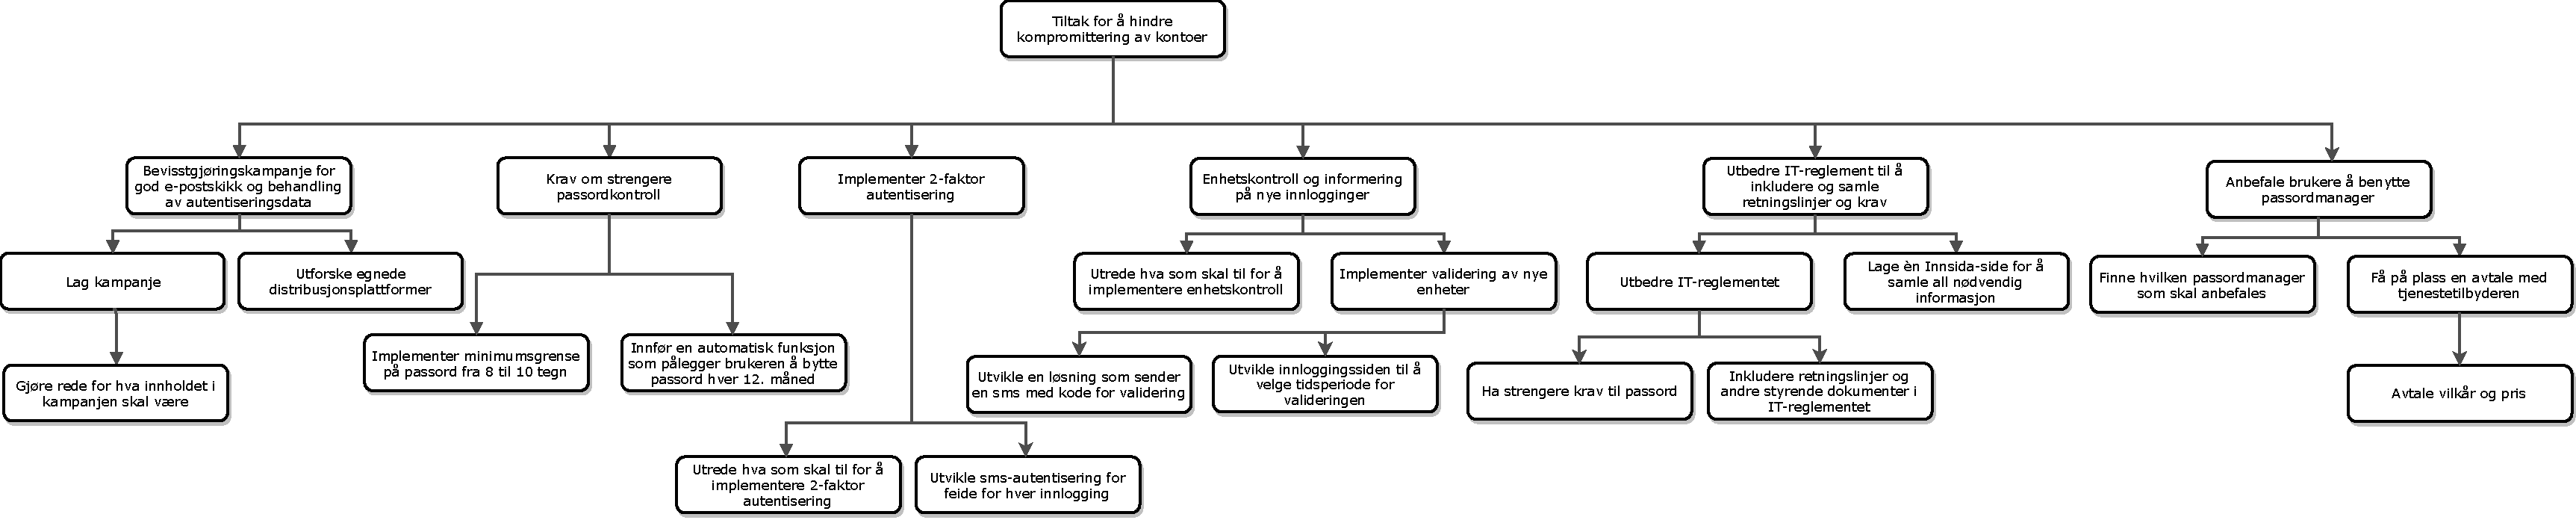
\includegraphics[scale=0.4, angle=90]{case_2/bilder/trediagram.pdf}
    \caption[Trediagram av tiltak mot kompromitterte kontoer]{Trediagram av tiltak mot kompromitterte kontoer}
    \label{fig:trediagram-case2}
\end{figure}

\section{Kostnad-nytte-analyse}
Denne seksjonen tar for seg en kostnad-nytte-analyse av nytteverdien til bruk av rotårsaksanalyse for case 2. 

\subsection{Kostnad for gjennomføring}
I denne analysen definerer vi kostnad som tid brukt på en iterasjonen av metoden. Vi definerer en skala for kostnad fra 1 til 5 der nivåene tilsvarer følgende tidsbruk:

\begin{enumerate}
    \item Under 50 timer
    \item 50-150 timer
    \item 150-250 timer
    \item 250-400 timer
    \item Over 400 timer
\end{enumerate}

Tabell \ref{tab:tidsbruk_case2} under viser tidsbruken i enkeltfasene i dette caset. Dette inkluderer tid brukt til å dokumentere alt som har med de enkelte fasene å gjøre. 

% Table generated by Excel2LaTeX from sheet 'Ark1'
\begin{table}[H]
  \centering
  \caption{Tidsbruk i de ulike fasene i case 2}
    \begin{tabular}{|lr|l|}
    \hline
    \multicolumn{3}{|c|}{\cellcolor{yellow}\textbf{Case 2}} \\
    \hline
    \multicolumn{1}{|l|}{\cellcolor{apricot}\textbf{Fase}} & \multicolumn{1}{l|}{\cellcolor{apricot}\textbf{Verktøy brukt}} & \cellcolor{apricot}\textbf{Timer totalt} \\
    \hline
    \multicolumn{1}{|l|}{Problemforståelse} & \multicolumn{1}{l|}{Kritiske hendelser} & 14-18t \\
    \hline
    \multicolumn{1}{|l|}{Idémyldring} & \multicolumn{1}{l|}{Idemyldring} & 14-18t \\
    \hline
    \multicolumn{1}{|l|}{Datainnsamling} & \multicolumn{1}{l|}{Sampling og spørreundersøkelse} & 70-90t \\
    \hline
    \multicolumn{1}{|l|}{Datanalyse} & \multicolumn{1}{l|}{Analyseverktøy} & 90-110t \\
    \hline
    \multicolumn{1}{|l|}{Rotårsaksidentifisering} & \multicolumn{1}{l|}{Årsak-virkningsdiagram og 5 Whys} & 18-22t \\
    \hline
    \multicolumn{1}{|l|}{Rotårsakseliminering} & \multicolumn{1}{l|}{SIT} & 14-18t \\
    \hline
    \multicolumn{1}{|l|}{Løsningsimplementering} & \multicolumn{1}{l|}{Trediagram} & 8-10t \\
    \hline
    \multicolumn{2}{|l|}{\textbf{Sum}} & \textbf{228-286t} \\
    \hline
    \end{tabular}%
  \label{tab:tidsbruk_case2}%
\end{table}%

Dersom kosten på caset går over flere nivåer regner vi med medianen til ytterpunktene for å plassere kostnaden. Basert på kostnadsnivåene vi definerte over, plasseres tidsbruken på case 2 til:
\[Kostnad = 4\]

\subsection{Nytte av resultatene}
I denne analysen definerer vi nytten som egen oppfatning av hvor gode resultatene fra caset var. Det vurderes ut fra om vi tror det kan finnes andre underliggende årsaker, og hvorvidt vi mener problemet blir løst dersom rotårsakene fjernes. Nytten defineres på en skala fra 1 til 5. 

I dette caset kom vi frem til at rotårsakene var spredt over flere årsaker. Hovedårsakene var gjenbruk av kredentialier på flere tjenester, phishing og utilstrekkelig tilgangskontroll på brukerkontoene. Vi er sikre på at hvis disse årsakene fjernes, vil brorparten av problemet løses. Vi definerer derfor nytten til:
\[Nytte = 5\]

\subsection{Total nytteverdi}
Når vi regner ut kostnad-nytte deler vi kostnaden på nytteverdien. 
\[\frac{Kostnad}{Nytte} = Total nytteverdi\]

I dette caset blir regnestykket slik:
\[\frac{4}{5} = 0,8\]

Svarene på regnestykket kan bli fra 0,2 til 5. Jo lavere denne nytteverdien er, jo bedre fungerte metoden til caset. 
\chapter{Resultater og analyse fra Case 3: Misbruk av NTNU sin infrastruktur til utvinning av kryptovaluta}
I dette kapittelet fremlegger vi våre resultater i alle fasene i case 3.
%%%%%%%%%%%%%%%%%%%%%%%%%%%%%%%%%%%%%%%%%%%%%%%%%%%%%%%%%%%%%%%%%%%%%
\section{Problemforståelse}
\subsection{Ytelsesmatrise}
Variablene som ble vurdert til å kunne hjelpe til å redusere utvinning av kryptovaluta hos NTNU er som følger:
\begin{description}
    \item[Adgangskontroll på HPC klynger:] Klynger av tilkoblet maskinvare som sammen utgir svært høy ytelse. Er også kjent som superdatamaskiner. Disse er godt beskyttet med streng adgangskontroll og logging av alt som blir gjort.
    \item[Adgangskontroll på kritiske servere:] Adgangskontroll til servere som har en funksjonskritisk og/eller virksomhetskritisk rolle i driften av NTNU, som for eksempel DNS og DHCP servere. 
    \item[Adgangskontroll på andre servere:] Adgangskontroll til alle servere som ikke har en kritisk rolle i NTNU, men som fortsatt kan bli misbrukt. Inkluderer servere som står åpent ut mot nettet. 
    \item[Beskyttelse mot ufrivillig utvinning på datamaskiner:] Beskyttelse mot at personer får tilgang til din datamaskin gjennom nettleseren og bruker den til å utvinne kryptovaluta. 
    \item[Policy på hva som er akseptabelt som BYOD:] Definerer hva som er lov å ta med av BYOD.
    \item[IT-reglement på krypto utvinning:] IT-reglementet spesifiserer per i dag bare at det å misbruke universitetets ressurser til kommersiell virksomhet ikke er greit. Det kan være vanskelig for folk å skjønne at strøm er en slik ressurs og at utvinning av kryptovaluta kan regnes som kommersiell virksomhet. Slik som IT-reglementet er idag er det heller ikke noen gode sanksjonsmuligheter mot folk som utvinner kryptovaluta.
\end{description}

Under ser vi hvor de ulike ressursene, eller aktiva, er plassert i henhold til de tidligere nevnte områdene.
\begin{figure}[H]
    \centering
    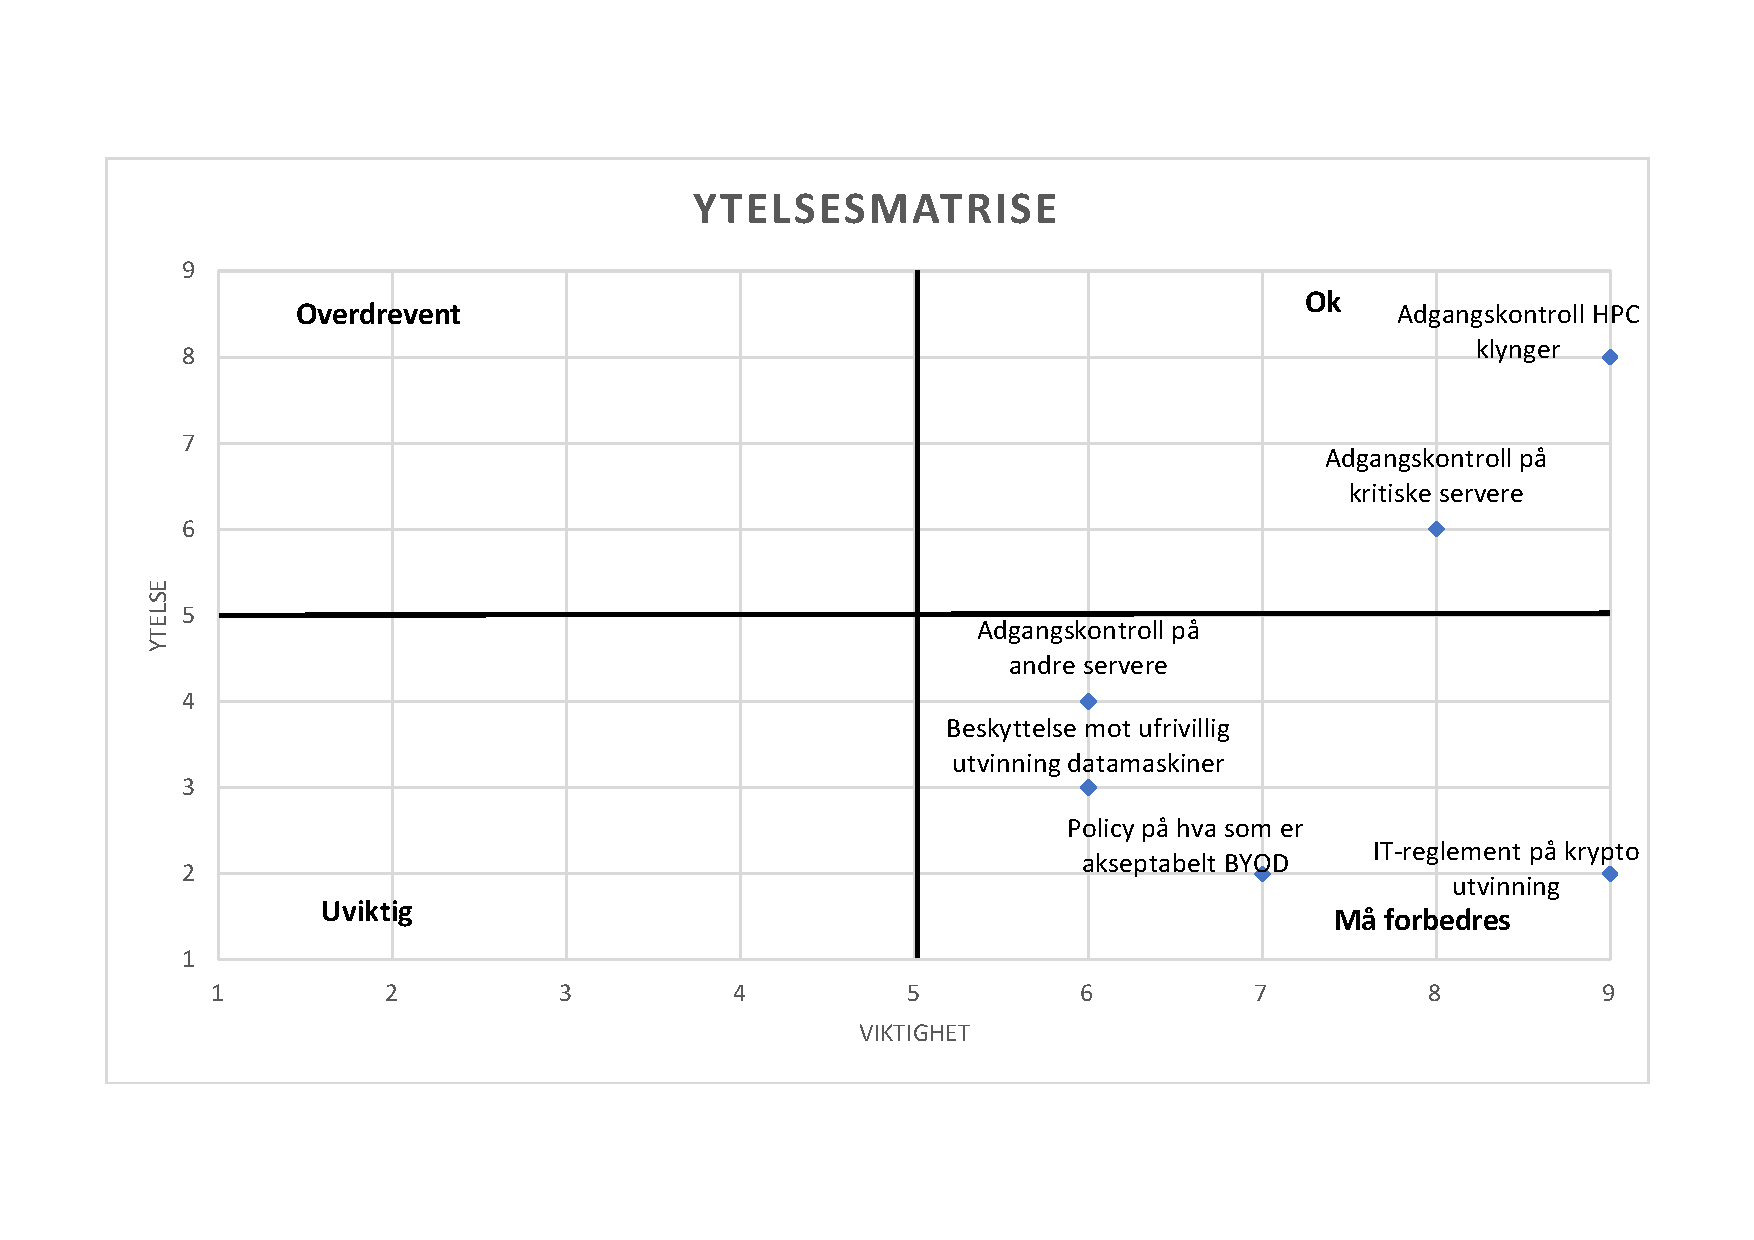
\includegraphics[scale=0.5]{case_3/bilder/ytelsesmatrise.pdf}
    \caption[Ytelsesmatrise]{Resultater fra ytelsesmatrisen}
    \label{fig:ytelsesmatrise}
\end{figure}

Det er mest kritisk å vurdere de variablene som havner under ``må forbedres''. Selv om noen havner under ``ok'', bør de fortsatt vurderes, men de vil ha lavere prioritet enn de nevnt over. Variabler som er uviktig eller overdrevent trenger man ikke vurdere nøye. Matrisen viser følgende prioriteringsgrunnlag til utbedring:

\begin{enumerate}
    \item IT-reglement på krypto utvinning
    \item Policy på hva som er akseptabelt som BYOD
    \item Beskyttelse mot ufrivillig utvinning på datamaskiner
    \item Adgangskontroll på andre servere
    \item Adgangskontroll på kritiske servere
    \item Adgangskontroll på HPC klynger
\end{enumerate}

%%%%%%%%%%%%%%%%%%%%%%%%%%%%%%%%%%%%%%%%%%%%%%%%%%%%%%%%%%%%%%%%%%%%%
\section{Idémyldring}
\subsection{Idémyldring}
Etter at idémyldringsøkten var ferdig ble det gjort en vurdering av hvilke momenter som hørte sammen eller hadde likhetstrekk.  Disse ble gruppert sammen, se figur \ref{fig:idemyldring-hvordan} og \ref{fig:idemyldring-hvorfor} under.

\begin{figure}[H]
    \centering
    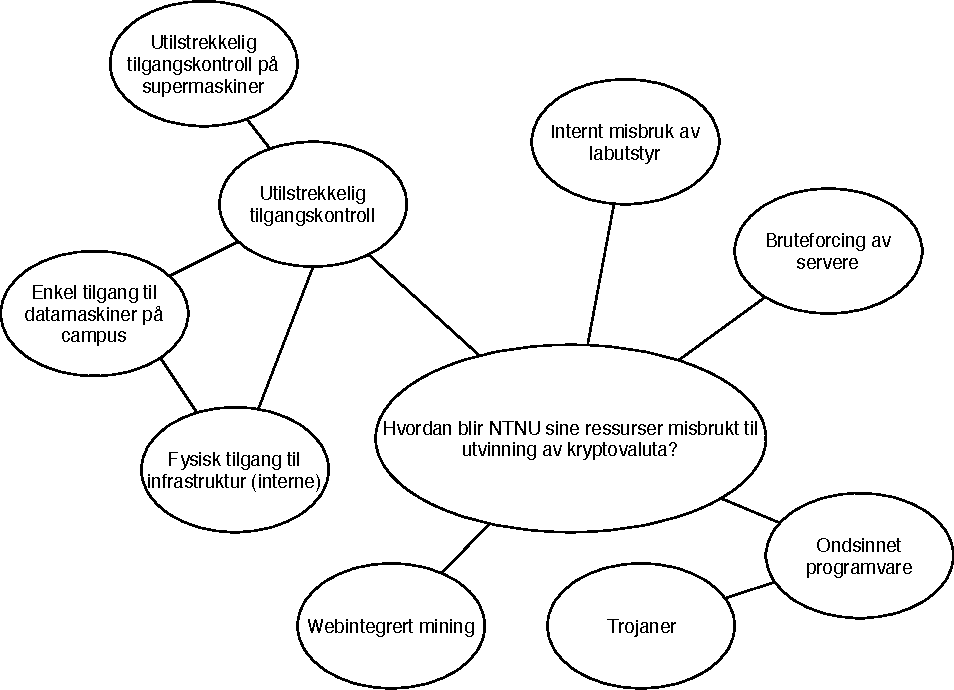
\includegraphics[scale=0.6]{case_3/bilder/idemyldring-hvordan.pdf}
    \caption[Idémyldring]{Resultater og gruppering av Hvordan}
     \label{fig:idemyldring-hvordan}
\end{figure}

\begin{figure}[H]
    \centering
    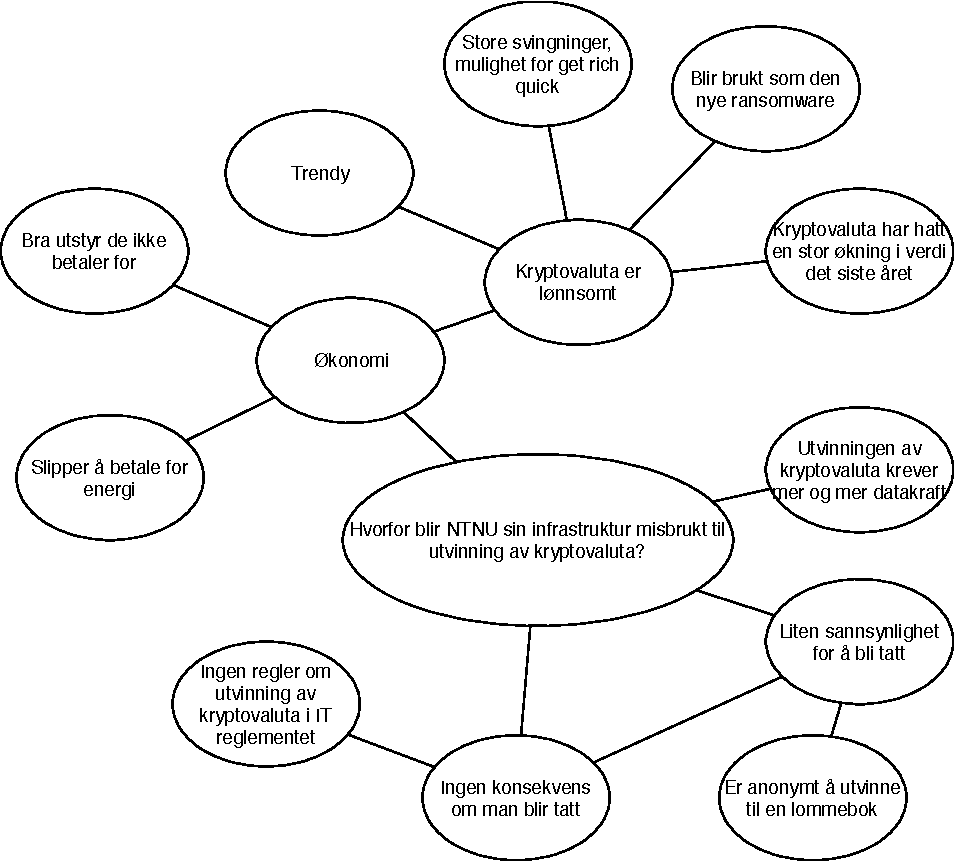
\includegraphics[scale=0.6]{case_3/bilder/idemyldring-hvorfor.pdf}
    \caption[Idémyldring]{Resultater og gruppering av Hvorfor}
    \label{fig:idemyldring-hvorfor}
\end{figure}

Resultatene er gruppert inn i 4 hovedkategorier:
\begin{description}
    \item [Ondsinnet programmvare] Er i stor grad trojanere i form av javascript.
    \item [Utilstrekkelig tilgangskontroll] Tilganskontroll på diverese datamaskiner rundt på campus, som kan utnyttes.
    \item [Økonomi] Er i stor grad motivasjonen til aktørene, der det er stor økonomisk vinning med kryptovaluta.
    \item[Ingen konsekvens om man blir tatt] Det står lite i IT-reglementet om at krypto utvinning ikke er lov.
\end{description}

\subsection{NGT}
Etter at hvert gruppemedlem hadde gitt ut sine 15 poeng satt vi igjen med 4 idéer som stakk seg ut med hvor mange poeng de fikk. Disse vises i fet skrift i tabell \ref{tab:NGT}. 

\begin{table} [H]
    \begin{tabular}{ | m{2em} | m{30em} | m{3em} | }
        \hline
            \cellcolor{yellow}  & \cellcolor{yellow} \textbf{Årsak} & \cellcolor{yellow} Poeng \\
        \hline
           A& Bra utstyr de ikke betaler for & 5 \\
        \hline
          B & Bruteforce av servere & 0 \\
        \hline
          C & Enkel tilgang til datamaskiner på campus & 0 \\
        \hline
         \textbf{D} & \textbf{Ingen regler om utvinning av kryptovaluta i IT reglementet} & 11 \\
        \hline
          \textbf{E} & \textbf{Internt misbruk av labutstyr} & 8  \\
        \hline
          F & Kryptovaluta har hatt en stor økning i verdi det siste året & 0 \\
        \hline
         G & Liten sannsynlighet for å bli tatt & 2 \\
        \hline
         \textbf{H} & \textbf{Ondsinnet programvare som utvinner} &  16 \\
        \hline
         I & Slipper å betale for energi & 0 \\
        \hline
         J & Store svingninger, mulighet for “get rich quick" & 0 \\
        \hline
         K & Utilstrekkelig tilgangskontroll på supermaskiner & 0 \\
        \hline
         L & Utvinningen av kryptovaluta krever mer og mer datakraft & 4 \\
        \hline
         \textbf{M} & \textbf{Kryptoutvinner integrert i nettleser} & 14 \\
        \hline
    \end{tabular}
    \caption{Oversikt over prioritering av idéer ved hjelp av NGT}
    \label{tab:NGT}
\end{table}

Disse fire årsakene er de vi kommer til å fokusere på i dette caset. De fire fokuspunktene kan deles etter de to problemstillingene ``hvordan og hvorfor''.

De to årsakene knyttet til ``hvorfor'' går ut på at det ikke er ulovlig med kryptoutvinning i henhold til gjeldende regelverk \cite{ITReg}. De faller derfor i en gråsone der en ikke får noen represalier for å holde på med kryptoutvinning, annet enn å bli kastet av nettet. Konsekvensene får man hvis en utnytter NTNU sine ressurser til egen vinning.

De neste årsakene går ut på hvilke aktører som bruker universitetet sine ressurser til utvinning av kryptovaluta, og hvordan de bruker ressursene. Internt misbruk av labutstyr går ut på at studenter eller ansatte har tilgang til diverse labber og PCer som kan brukes til utvinning av kryptovaluta. Både ondsinnet programvare som utvinner kryptovaluta og kryptoutvinnere integrert i nettleser brukes av eksterne trusselaktører. Pengene som tjenes her går til kriminelle. Utvinning av kryptovaluta har blitt mer utbredt som et alternativ til løsepengevirus, der løsepengevirus har blitt mindre lønnsomt den siste tiden \cite{RW}.

%%%%%%%%%%%%%%%%%%%%%%%%%%%%%%%%%%%%%%%%%%%%%%%%%%%%%%%%%%%%%%%%%%%%%
\section{Datainnsamling}
\subsection{Spørreundersøkelse}
Før intervjuet fikk vi et utdrag av alarmer som SOCen får av de kjente signaturene som omhandler kryotoutvinning. Disse alarmene stammer fra kryptoutvinnere som folk har fått lagt inn på PCene sine, kryptoutvinnere i nettleser som er lagt inn på diverse nettsteder eller trojanere. 

Vi hadde noen hypoteser når vi utformet intervjuspørsmålene, disse var:
\begin{itemize}
    \item Det er tekniske løsninger som kan brukes til å fikse store deler av problemet.
    \item Det er begrenset handlingsrom for hva som kan bli gjort mot interne som utvinner.
    \item Lite bevissthet rundt regelverket til NTNU angående bruk av universitetets ressurser.
    \item Utviklingen av utvinning følger kryptovalutaen sin verdi.
    \item Dataer blir kompromittert gjennom de vanlige formene, phishing og wateringholes.
\end{itemize}

\begin{table}[H]
    \centering
    \begin{tabular}{|m{30em}|} 
        \hline
        \cellcolor{yellow} Spørsmål  \\
        \hline
        Hva er de typiske angrepsvektorene?  \\
        \hline
        Tar det lang tid å oppdage trojanere i nettverket? \\ 
        \hline
        Hva gjør Seksjon for Digital Sikkerhet når de oppdager trojanere? \\
        \hline
        Hvordan fant dere ut om HPC clusterne blir misbrukt? \\
        \hline
        Hvordan fant dere ut at det var internt misbruk?\\
        \hline
        Har dere andre tiltak enn å stenge internett til de som miner? \\
        \hline
        hva er grunnen til at dere ikke har implementert noe slike tiltak? \\
        \hline
        Hva tror du er oppfatningen blant dine kolleger er angående utvinning. Vet folk det er ulovlig eller har de ikke tenkt så mye over det og utvinner fordi det er en trend? \\
        \hline
        Hva er måten dere for du snakket tidligere om at dere så mange av de lommebøkene som ble brukt var fra mørke siden av nettet?  \\
        \hline
        Hvordan ser dere at de går til disse lommebøkene? \\
        \hline
        Hvordan skal dere implementere kryptoutvinning i neste IT-reglement? \\
        \hline
        Tenker folk over at det ikke er lov til å utvinne krypto i henhold til IT-reglementet? \\
        \hline
        Har dere noen tiltak på utvinning på nettsider? \\
        \hline
        Er det like stor økning nå som det var før jul? \\
        \hline
        Økningen er det gjort av de profesjonelle aktørene eller er det folk som setter frivillig opp utvinnere? \\
        \hline
        Dere hadde ikke sett noe tilfeller av bruteforcede PCer og servere som ble installert kryptominere på, etter at de ble bruteforcet?  \\
        \hline
        Er det noen regler på hva ansatte får lov til å legge på serverne? \\
        \hline
        Har dere noen tilfeller av PCer på datalabber der studenter har installert kryptoutvinning? \\
        \hline
    \end{tabular}
    \caption{Spørsmål til intervju case 3}
    \label{tab:spm-intervju}
\end{table}
Under intervjuet ble det tatt lydopptak, slik at vi lett kunne gå tilbake til svarene for å få det mest mulig nøyaktig til neste fase. Når intervjuet var ferdig ble det transkribert. Transkripsjonen finnes i vedlegg \ref{transkripsjon}.
%%%%%%%%%%%%%%%%%%%%%%%%%%%%%%%%%%%%%%%%%%%%%%%%%%%%%%%%%%%%%%%%%%%%%
\section{Dataanalyse}
\subsection{Affinitetsdiagram}
Affinitetsdiagram brukes til å analysere data som det ikke er mulig å nummerere, eksempelvis meninger eller idéer. Affinitetsdiagram grupperer data og finner de underliggende korrelasjoner og likhetstrekk i gruppen.

Analysen ble gjennomført med å ta transkripsjon av intervjuet og stykke den opp i fem hovedgrupper.     

\begin{figure}[H]
    \centering
    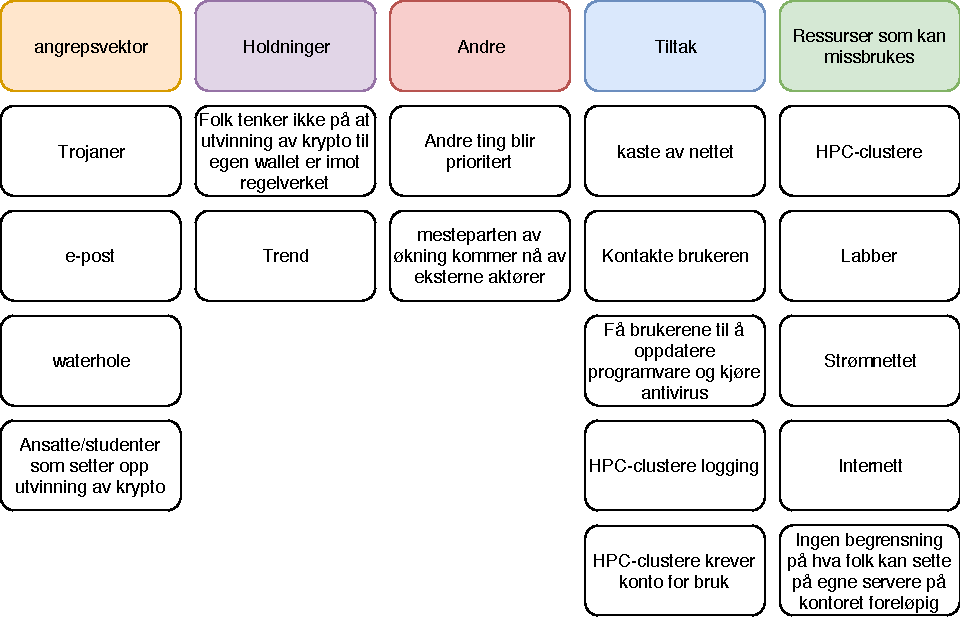
\includegraphics[scale=0.6]{case_3/bilder/AD.pdf}
    \label{fig:AD_miner}
    \caption{Hvordan fungerer utvinning av kryptovaluta ved NTNU?}
\end{figure}

Affinitetsdiagrammet deles inn i hovedkategoriene: angrepsvektor, holdninger, ressurser som kan misbrukes, tiltak og andre. Blant disse er mulige årsaker til problemet og anbefalte tiltak som kan løse det. 



%RESULTAT for affinitetsdiagram.

%%%%%%%%%%%%%%%%%%%%%%%%%%%%%%%%%%%%%%%%%%%%%%%%%%%%%%%%%%%%%%%%%%%%%
\section{Rotårsaksidentifisering}
\subsection{5 whys}
Det ble fremhevet fem årsaker som skulle analyseres. Fire av disse kom fra fiskebeindiagrammet over, og en fra idémyldring. Tabellene under viser resultatene fra gjennomføringen. 

\begin{table} [H]
    \centering
    \begin{tabular}{ | m{5em} | m{30em} | }
        \hline
            \cellcolor{yellow} Årsak: & \cellcolor{yellow} Ansatte og studenter utvinner krypto med universitetet sine ressurser                \\
        \hline
            Why? & Lønnsomhet                                    \\
        \hline
            Why? & Har ingen utgifter                                            \\
        \hline
            Why? & Bruker strøm og infrastrukturen til skolen                \\
        \hline
            Why? & Det er en gråsone i regelverket           \\
        \hline
            Why? & Ikke spesifisert godt nok i IT-reglementet   \\
        \hline
    \end{tabular}
    \caption[5 Whys: Ansatte og studenter utvinner krypto med skolens]{5 Whys på ansatte og studenter utvinner krypto med skolens}
    \label{5Whys-interne}
\end{table}
Det å utvinne krypto på universitetet sine ressurser er alt fra å kjøre en kryptoutvinner på en PC til å sette opp maskinvare ment for kryptoutvinning. I 5 Whys over kom vi frem til at lønnsomhet er primærgrunnen til at de driver med kryptoutvinning, men årsaken til at ansatte og studenter utvinner på universitet er at det ikke er spesifisert godt nok i IT-reglementet.   


\begin{table} [H]
    \centering
    \begin{tabular}{ | m{5em} | m{30em} | }
        \hline
            \cellcolor{yellow} Årsak: & \cellcolor{yellow} Eksterne trusselaktører utvinner kryptovaluta med skolens ressurser              \\
        \hline
            Why? & Lønnsomhet                                   \\
        \hline
            Why? & Enkelt å spre minere                                           \\
        \hline
            Why? & Folk går inn på waterholes og trykker på phishingmail               \\
        \hline
            Why? & Brukeren var ikke oppmerksom nok på e-post eller siden de gikk på           \\
        \hline
            Why? & Brukere har ikke fått nok opplæring i hvordan dette unngås    \\
        \hline
    \end{tabular}
    \caption[5 Whys: Eksterne trusselaktører utvinner kryptovaluta med skolens ressurser]{5 Whys Eksterne trusselaktører utvinner kryptovaluta med skolens ressurser}
    \label{5Whys-eksterne}
\end{table}

Årsaken til at eksterne trusselaktører utvinner kryptovaluta med universitetet sine ressurser er fordi det er en lønnsom affære som koster lite å distribuere og som det er liten sannsynlighet å bli tatt for. Dette virker i kombinasjon med at brukere ikke er oppmerksom på hva de trykker på. Rotårsaken til at de ikke er oppmerksomme er at de ikke har fått nok opplæring.

\begin{table} [H]
    \centering
    \begin{tabular}{ | m{5em} | m{30em} | }
        \hline
            \cellcolor{yellow} Årsak: & \cellcolor{yellow} Utvinnere som implementert inn i nettsider              \\
        \hline
            Why? & God fortjeneste                                   \\
        \hline
            Why? & Fordi de når en stor menge folk som utvinner kryptovaluta for dem                                           \\
        \hline
            Why? & Mange har ikke en annonseblokkering som også stopper utvinnere på nett               \\
        \hline
            Why? & På grunn av lite eller ingen opplæring til denne typen programvare           \\
        \hline
            Why? & Ikke prioritert    \\
        \hline
            Why? & Fordi det ikke er nok folk/ressurser    \\
        \hline
    \end{tabular}
    \caption[5 Whys: Minere som er implementert inn i nettsider]{5 Whys på ansatte og studenter utvinner kryptovaluta med skolens}
    \label{5Whys-minere}
\end{table}

Utvinning på nettsider blir mer utbredt fordi det er profitabelt og en god erstatning til reklame. Dette kan bli stoppet med annonseblokkering eller blokkering av DNS adresser. Dette blir ikke gjort fordi det ikke er en prioritet fra seksjon for digital sikkerhet.

\subsection{Feiltreanalyse}
Feiltreanalyse tar for seg alle mulige årsaker i et diagram og identifiserer mulige relasjoner. Analysen bygger på hva som ble gjort i 5 Whys.

Vi har kommet fram til fire hovedgrunner til at kryptoutvinning på NTNU forekommer. Rotårsaken er sammensatt av årsakene definert i figur \ref{fig:feil_tre_analyse}. I dette caset er problemet delt inn i to deler: de interne og de eksterne. Det er to forskjellige typer årsaker, der interne går mer på regelverk og eksterne er mer teknisk. 

 \begin{figure}[H]
    \centering
    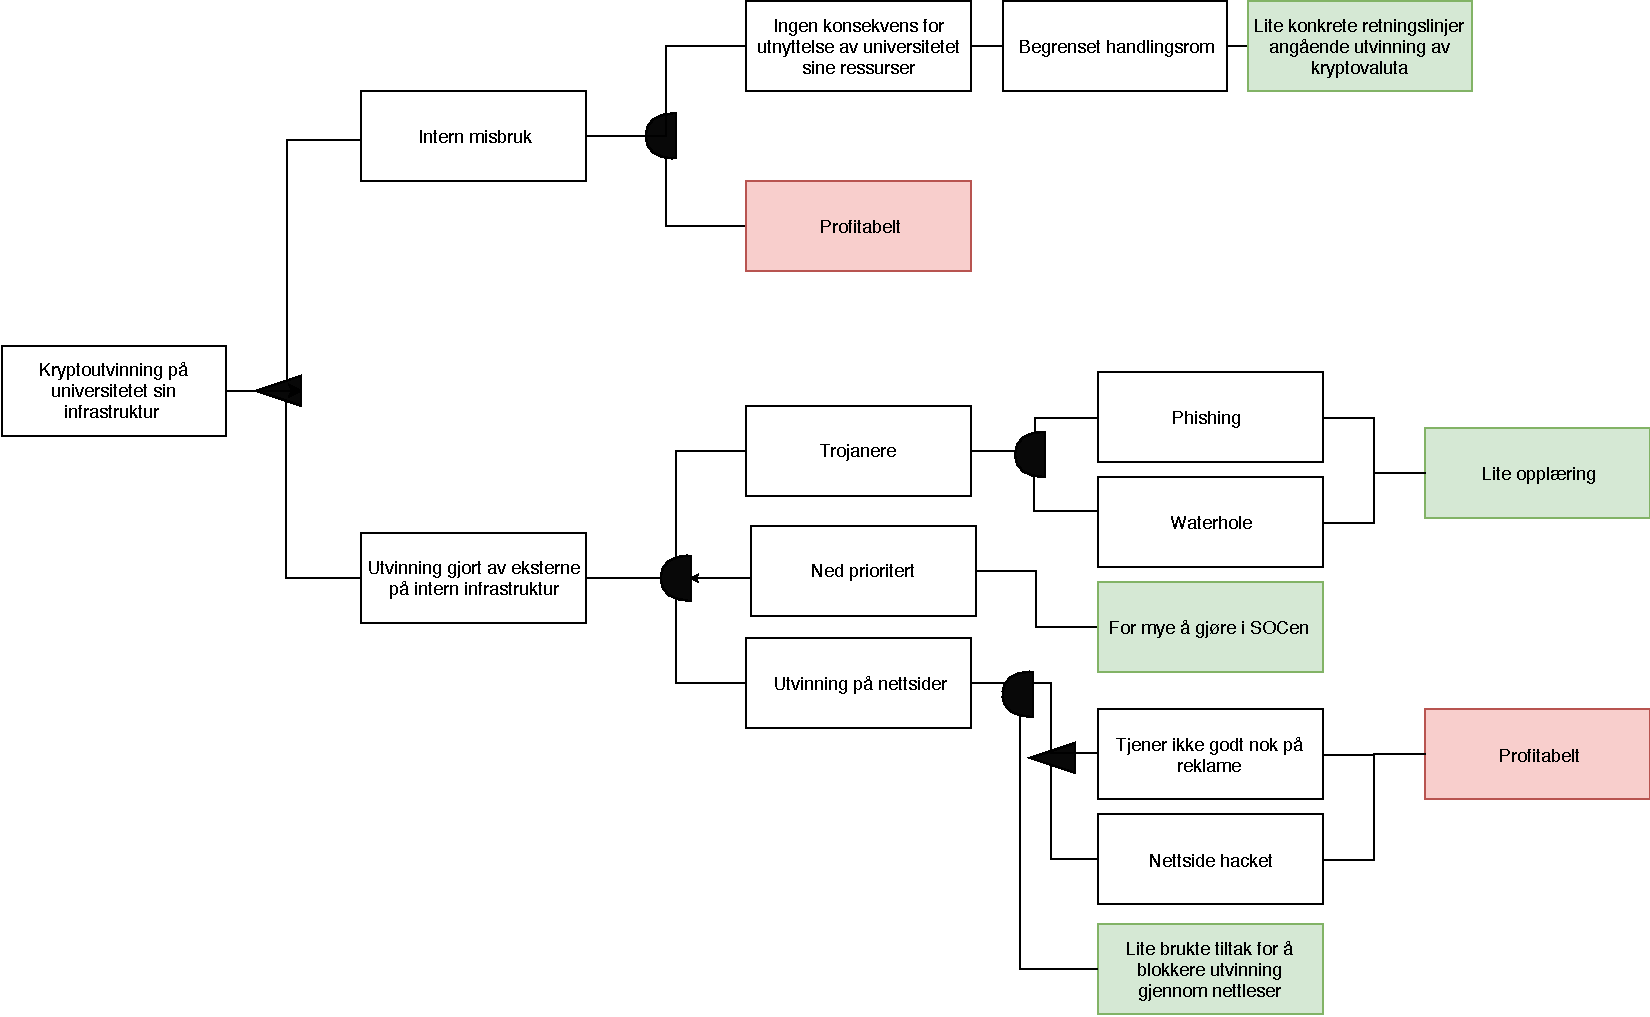
\includegraphics[scale=0.45]{case_3/bilder/feil_tre_analyse.pdf}
    \caption{Feiltreanalyse}
    \label{fig:feil_tre_analyse}
\end{figure}

I figur \ref{fig:feil_tre_analyse} over representerer trekanter ``eller'' og halvsirkelen ``og''. De røde boksene er de årsakene vi ikke kan gjøre noe med, mens de grønne kan det gjøres noe med.
%%%%%%%%%%%%%%%%%%%%%%%%%%%%%%%%%%%%%%%%%%%%%%%%%%%%%%%%%%%%%%%%%%%%%
\section{Rotårsakseliminering}
\subsection{SIT}
Alle komponenter som eksisterer i problemets naturlige omgivelser listes under:

\begin{itemize}
    \item IT-reglement
    \item Annonseblokker
    \item Internett
    \item SOCen
    \item Brannmur
    \item Servere og datamaskiner
    \item Datalabber
    \item HPC-cluster
    \item Bring your own device (BYOD)
    \item Strøm
\end{itemize}

Når komponentene er gjort rede for, vil de fem SIT prinsippene brukes sekvensielt på komponentene for å utvikle løsninger på problemene. Ikke alle SIT-prinsipper finner løsninger som er gjennomførbare for alle komponenter. I disse tilfellene vil det stå: ``Ikke gjennomførbart''. Resultatene fremheves under.

\paragraph{IT-reglement}
\begin{itemize}
    \item \textbf{Attributtavhengighet} Legge til et større fokus på utvinning av kryptovaluta.
    \item \textbf{Komponentkontroll} Gjennomføre en informasjonskampanje for å sette fokus på hva som er misbruk.
    \item \textbf{Erstatning} Ikke gjennomførbart.
    \item \textbf{Forkastning} Ikke gjennomførbart.
    \item \textbf{Oppdeling} Ikke gjennomførbart. 
\end{itemize}

\paragraph{Annonseblokker}
\begin{itemize}
    \item \textbf{Attributtavhengighet} Legge til blokkering av kryptoutvinning 
    \item \textbf{Komponentkontroll} Passe på at alle ansatte har annonseblokker installert som også stopper utvinning av kryptovaluta.
    \item \textbf{Erstatning} Ikke gjennomførtbart
    \item \textbf{Forkastning} Ikke gjennomførtbart
    \item \textbf{Oppdeling} Ikke gjennomførtbart.
\end{itemize}

\paragraph{Internett}
\begin{itemize}
    \item \textbf{Attributtavhengighet} Blokkere kryptoutvinning
    \item \textbf{Komponentkontroll} Automatisere at alle datamaskiner som utvinner kryptovaluta blir kastet av nettet.
    \item \textbf{Erstatning} Ikke gjennomførtbart.
    \item \textbf{Forkastning} Ikke gjennomførtbart.
    \item \textbf{Oppdeling} Ikke gjennomførtbart.
\end{itemize}


\paragraph{SOC}
\begin{itemize}
    \item \textbf{Attributtavhengighet} Øke antall ansatte.
    \item \textbf{Komponentkontroll} Økt prioritet til kryptovaluta.
    \item \textbf{Erstatning} Ikke gjennomførtbart.
    \item \textbf{Forkastning} Ikke gjennomførtbart.
    \item \textbf{Oppdeling} Gi forslag til implementering av tiltak til bachelorgrupper.
\end{itemize}

\paragraph{Servere og datamaskin}
\begin{itemize}
    \item \textbf{Attributtavhengighet} Strengere adgangskontroll.
    \item \textbf{Komponentkontroll} Ikke gjennomførtbart.
    \item \textbf{Erstatning} Ikke gjennomførtbart.
    \item \textbf{Forkastning} Ikke gjennomførtbart.
    \item \textbf{Oppdeling} Ikke gjennomførtbart.
\end{itemize}

\paragraph{Datalabber}
\begin{itemize}
    \item \textbf{Attributtavhengighet} Strengere adgangskontroll.
    \item \textbf{Komponentkontroll} Logging.
    \item \textbf{Erstatning} Svakere maskinvare på labbene.
    \item \textbf{Forkastning} Slutte å tilby labber, som kan brukes i sammenheng med kryptoutvinning.
    \item \textbf{Oppdeling} Ikke gjennomførbart.
\end{itemize}

\paragraph{HPC-clustere}
\begin{itemize}
    \item \textbf{Attributtavhengighet} Øke tilgangskontrollen ytterligere.
    \item \textbf{Komponentkontroll} Ikke gjennomførbart.
    \item \textbf{Erstatning} Ikke gjennomførbart.
    \item \textbf{Forkastning} Ikke gjennomførbart.
    \item \textbf{Oppdeling} Ikke gjennomførbart.
\end{itemize}


\paragraph{Bring your own device (BYOD)}
\begin{itemize}
    \item \textbf{Attributtavhengighet} Ikke gjennomførbart.
    \item \textbf{Komponentkontroll} Kaste datamaskiner som ikke tilhører NTNU-personell av nettet slik at de manuelt må koble seg på igjen.
    \item \textbf{Erstatning} Ikke gjennomførbart.
    \item \textbf{Forkastning} Ikke gjennomførbart.
    \item \textbf{Oppdeling} Ikke gjennomførbart.
\end{itemize}

\paragraph{Strøm}
\begin{itemize}
    \item \textbf{Attributtavhengighet} Ikke gjennomførtbart
    \item \textbf{Komponentkontroll} Strømkvotering, overstiges kvoten må vedkommende betale for strømmen
    \item \textbf{Erstatning} Ikke gjennomførtbart
    \item \textbf{Forkastning} Ikke gjennomførtbart
    \item \textbf{Oppdeling} Ikke gjennomførtbart
\end{itemize}

Vi sorterer og beskriver de mest relevante idéer til videre utdyping:

\begin{description}
\item[Gjennomføre en informasjonskampanje om kommersielt misbruk av NTNU sin infrastruktur] Kampanjen skal få frem at det å bruke NTNU sine ressurser til kommersiell virksomhet bryter IT-reglementet. I NTNU sine ressurser inkluderer strøm og internett. %(y)
\item[Legge til et større fokus på utvinning av krypto i IT-reglementet] Gi IT-reglement et større fokus på kryptoutvinning og gi klarere retningslinjer på hva som ikke er akseptabelt.
\item[Legge til annonseblokker som stopper utvinning] Aktivere blokkering av utvinningsprotokoll på annonseblokkere og passe på at alle har en annonseblokkeringstjeneste installert.
\item[Blokkere kryptoutvinning] Med dette mener vi å gjøre et eller flere tiltak som å blokkere DNS-forespørsler som omhandler kryptoutvinning.  
\item[Øke antall personell i SOC] SOC har mange oppgaver som er mer kritiske enn kryptoutvinning. Derfor foreslår vi å ansette flere, kanskje i kombinasjon med bacheloroppgaver.
\item[Strengere adgangskontroll] Begrenser tilgang til datalabber. 
\item[Logging] Øke bruk av logging i datalabbene. 
\item[Kaste datamaskiner som ikke er kritisk infrastruktur av nettet] Ved midnatt blir alle datamaskiner eller servere som ikke er kritisk infrastruktur koblet av nettet og må manuelt koble seg på nettet igjen.
\end{description}

\subsection{Tiltaksplan}
Etter å ha brukt de fem SIT-prinsippene på hver komponent og filtrert de, sitter vi igjen med et par idéer. I denne delen fremhever vi idéer i en tiltaksplan som vi anbefaler å implementere. 
Under beskrives de ulike tiltakene:

\begin{description}
    \item[Gjennomføre en informasjonskampanje om kommersielt misbruk av NTNU sin infrastruktur] Utvinning av kryptovaluta er en ny ting, hvor mange ikke er klar over hvordan universitetet sitt regelverk håndterer temaet. Vår anbefaling er å ha en kampanje der universitet informerer om hva som regnes som NTNU sine ressuser og hvordan disse ikke skal brukes til kommersiell virksomhet.
    \item[Legge til et større fokus på utvinning av krypto i IT-reglementet] Endre IT-reglementet slik at det blir tydelig at kryptoutvinning ikke er lovlig bruk av NTNU sine ressurser. 
    \item[Blokkere kryptoutvinning] Dette tiltaket går ut på å blokkere DNS-forespørsler tilknyttet kryptoutvinning. Slik at PCer som blir brukt i utvinning ikke kan hente nye oppgaver å løse. De velkjente DNS-ene blokkeres. Videre kan loggen bli benyttet for å legge nye domener inn i en svarteliste, eller justere de gamle DNS-ene.
    \item[Øke antall personell i SOC] SOCen kan ikke prioritere å stoppe utvinning av kryptovaluta. Derfor anbefaler vi å enten øke mengden personell i SOCen, eller gi utvikling av et teknisk forslag til implementasjon som en bacheloroppgave.
\end{description}

%%%%%%%%%%%%%%%%%%%%%%%%%%%%%%%%%%%%%%%%%%%%%%%%%%%%%%%%%%%%%%%%%%%%%
\section{Løsningsimplementering}
\subsection{Kraftfeltsanalyse} 
Kraftfeltsanalyse blir brukt for å få en oversikt over hvilke styrker som er for og hvilke styrker som er mot implementering av tiltakene. Dette verktøyet gir en plan over hvilke tiltak som er lettest å gjennomføre.  

Informasjonskampanjen og endringen i IT-reglementet bør gjøre i kombinasjon med hverandre. Der IT-reglementet får klartgjort at selv om kryptoutvinning ikke ulovlig i henhold til norsk lov, er det imot NTNU sitt IT-reglement så fremt det ikke er søkt om. Når endringen er gjort, gjennomføres informasjonskampanjen.   
Under, i tabell \ref{fig:kampanje} og \ref{fig:IT-reglement}, viser resultatene fra kraftfeltsanalysen på informasjonskampanje og endring i IT-reglementet.
 \begin{figure}[H]
    \hspace{2.2cm}
    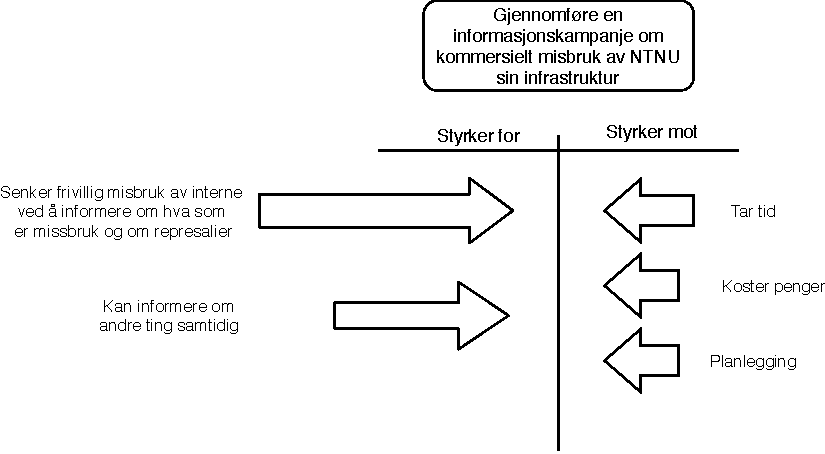
\includegraphics[scale=0.6]{case_3/bilder/Force-field1.pdf}
    \caption[Informasjonskampanje]{Oversikt over informasjonskampanjen }
    \label{fig:kampanje}
\end{figure}

 
 \begin{figure}[H]
    \hspace{2.6cm}
    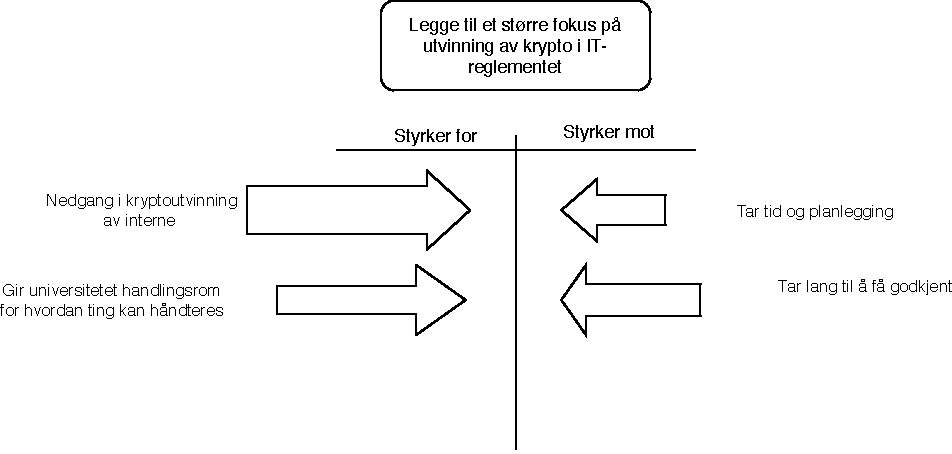
\includegraphics[scale=0.6]{case_3/bilder/Force-field2.pdf}
    \caption[Endre IT-reglementet]{Endring i IT-reglementet}
    \label{fig:IT-reglement}
\end{figure}

Fra dataanalysen kom vi frem til at selv om det finnes tekniske løsninger, har ikke SOCen hatt mulighet til å implementere DNS blokkering på bakgrunn av mangel på ressurser. Figur \ref{fig:Blokkering} og \ref{fig:Oke-antall} viser hva som skal til for å blokkere DNS og hva som må til for å øke ressursene til SOCen. Vi estimerer at den største kraften mot implementering av dette kommer til å være tidsbruk og kostnadene rundt tidsbruk.    
 \begin{figure}[H]
    \centering
    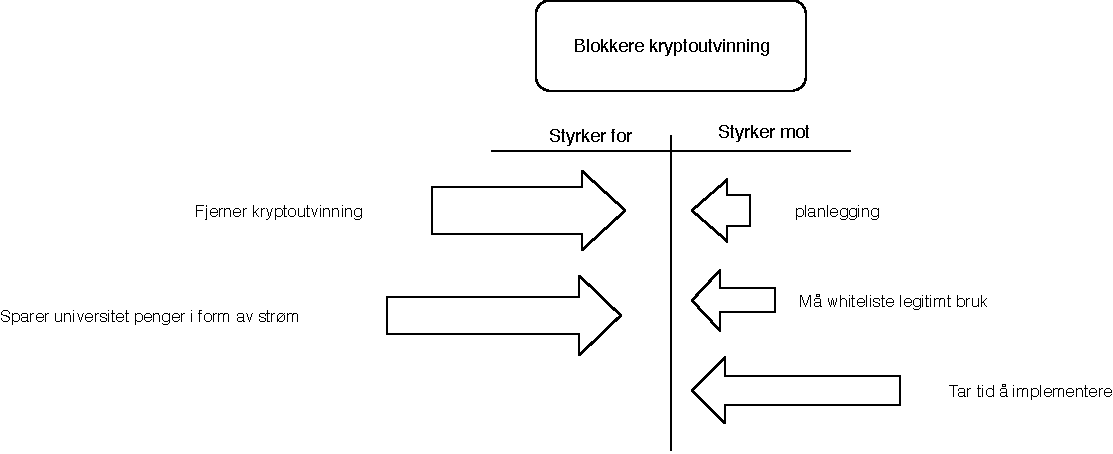
\includegraphics[scale=0.6]{case_3/bilder/Force-Field3.pdf}
    \caption[Blokkering]{Blokkering av DNS forespørsel}
    \label{fig:Blokkering}
\end{figure}


Ved å øke antall ansatte i SOCen estimerer vi at kosten av en ny ansatt vil være største kraften mot. Det er vanskelig å si om vedkommende vil ha nok arbeidsoppgaver til at det er verdt ansettelsen. Det bør vurderes å gi prosjekter til bachelor- og masterstudenter. 
 \begin{figure}[H]
    \hspace{3.6cm}
    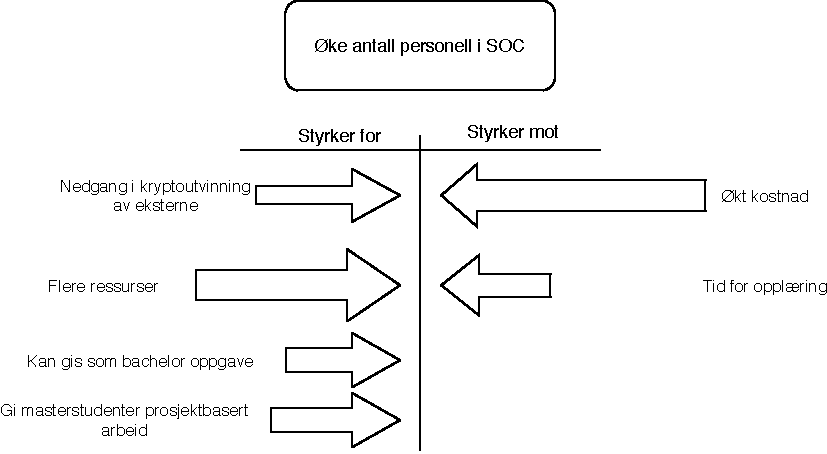
\includegraphics[scale=0.6]{case_3/bilder/Force-field4.pdf}
    \caption[Øke antall ansette i SOC]{Øke andel ansatte i SOC}
    \label{fig:Oke-antall}
\end{figure}

Figurene viser våres antakelser på hvilke krefter som jobber for implementeringen og hvilke som jobber mot, samt estimater på styrken til kreftene. Lengden på pilene indikerer antatt styrke. 
%%%%%%%%%%%%%%%%%%%%%%%%%%%%%%%%%%%%%%%%%%%%%%%%%%%%%%%%%%%%%%%%%%%%%
\section{Kostnad-nytte-analyse}
\label{kost-nytte-case3}
Denne seksjonen tar for seg en kostnad-nytte-analyse av nytteverdien til bruk av rotårsaksanalyse for case 3. 

\subsection{Kostnad for gjennomføring}
I denne analysen definerer vi kostnad som tid brukt på en iterasjonen av metoden. Vi definerer en skala for kostnad fra 1 til 5 der nivåene tilsvarer følgende tidsbruk:

\begin{enumerate}
    \item Under 50 timer
    \item 50-150 timer
    \item 150-250 timer
    \item 250-400 timer
    \item Over 400 timer
\end{enumerate}

Tabell \ref{tab:tidsbruk_case3} under viser tidsbruken i enkeltfasene i dette caset. Dette inkluderer tid brukt til å dokumentere alt som har med de enkelte fasene å gjøre. 

% Table generated by Excel2LaTeX from sheet 'Ark1'
\begin{table}[H]
  \centering
  \caption{Tidsbruk i de ulike fasene i case 3}
    \begin{tabular}{|lr|l|}
    \hline
    \multicolumn{3}{|c|}{\cellcolor{yellow}\textbf{Case 3}} \\
    \hline
    \multicolumn{1}{|l|}{\cellcolor{apricot}\textbf{Fase}} & \multicolumn{1}{l|}{\cellcolor{apricot}\textbf{Verktøy brukt}} & \cellcolor{apricot}\textbf{Timer totalt} \\
    \hline
    \multicolumn{1}{|l|}{Problemforståelse} & \multicolumn{1}{l|}{Ytelsesmatrise} & 16-20t \\
    \hline
    \multicolumn{1}{|l|}{Idémyldring} & \multicolumn{1}{l|}{Idémyldring og NGT} & 16-20t \\
    \hline
    \multicolumn{1}{|l|}{Datainnsamling} & \multicolumn{1}{l|}{Intervju} & 20-30t \\
    \hline
    \multicolumn{1}{|l|}{Datanalyse} & \multicolumn{1}{l|}{Affinitetsdiagram} & 15-20t \\
    \hline
    \multicolumn{1}{|l|}{Rotårsaksidentifisering} & \multicolumn{1}{l|}{5 whys og feil-tre diagram} & 25-30t \\
    \hline
    \multicolumn{1}{|l|}{Rotårsakseliminering} & \multicolumn{1}{l|}{SIT} & 15-20t \\
    \hline
    \multicolumn{1}{|l|}{Løsningsimplementering} & \multicolumn{1}{l|}{Kraftfeltsdiagram} & 10-15t \\
    \hline
    \multicolumn{2}{|l|}{\textbf{Sum}} & \textbf{117-155t} \\
    \hline
    \end{tabular}%
  \label{tab:tidsbruk_case3}%
\end{table}%

Dersom kosten på caset går over flere nivåer regner vi med medianen til ytterpunktene for å plassere kostnaden. Basert på kostnadsnivåene vi definerte over, plasseres tidsbruken på case 3 til:
\[Kostnad = 2\]

\subsection{Nytte av resultatene}
I denne analysen definerer vi nytten som egen oppfatning av hvor gode resultatene fra caset var. Det vurderes ut fra om vi tror det kan finnes andre underliggende årsaker, og hvorvidt vi mener problemet blir løst dersom rotårsakene fjernes. Nytten defineres på en skala fra 1 til 5. 

I dette caset kom vi frem til at rotårsakene var uklarhetet i IT reglement når det kommer til utvinning av kryptovaluta, samt for lite ressurser på Seksjon for Digital Sikkerhet for å gjøre noe med tekniske løsninger. Caset ble preget av svakt datagrunnlag, så vi har grunn til å tro at det kan være flere rotårsaker. Tiltakene vi kom frem til vil kunne hjelpe med å begrense konsekvensene til problemet, men vil trolig ikke fjerne det helt. Vi definerer derfor nytten til:
\[Nytte = 2\]

\subsection{Total nytteverdi}
Når vi regner ut kostnad-nytte deler vi kostnaden på nytteverdien. 
\[\frac{Kostnad}{Nytte} = Total nytteverdi\]

I dette caset blir regnestykket slik:
\[\frac{2}{2} = 1\]

Svarene på regnestykket kan bli fra 0,2 til 5. Jo lavere denne nytteverdien er, jo bedre fungerte metoden til caset. 
\chapter{Diskusjon}
\label{kap:diskusjon}
Utgangspunktet i denne drøftingen er hvorvidt rotårsakene vi kom frem til i hvert case er reelle rotårsaker som, hvis fjernet, vil fjerne symptomene helt. I tillegg ser vi på hvordan erfaringen fra de tre casene viser hvor godt rotårsaksanalyse fungerer innen informasjonssikkerhet, om det lønner seg å bruke og hvilke verktøy som fungerer best innen informasjonssikkerhet. 

\section{Hva er rotårsaken til at studenter laster ned opphavsrettsbeskyttet materiale?}
\subsection*{Rotårsak: Dårligere utvalg på alternative tjenester i Norge}
Ut fra vår analyse viser det seg at dette er hovedårsaken til at studenter laster ned ulovlig. Siden Netflix og de andre strømmetjenestene har inntatt markedet har filmer og serier blitt fordelt mellom tjenestene. Tjenestene ønsker også flest mulig orginale serier som bare finnes hos dem. Dette gjør at tilgjengeligheten på filmer og serier går ned, med mindre man abonnerer på alt. Men selv da får man ikke tilgang på alt. Mange filmer og serier er geografisk blokkert i Norge, som gjør tilgjengeligheten til et enda større problem. I musikkstrømmingsmiljøet er problemet noe mindre. Selv om ulovlig musikknedlasting ikke er borte, har det blitt redusert \cite{musikkstream}. Noe av grunnen til dette er at musikkbransjen er mer sentralisert i hvem som eier rettighetene, også kjent som et oligopol. Dette gjør det lettere for strømmetjenestene å skaffe lisenser for musikk, og kan tilby det folk trenger på ett sted. Det er også mye mindre orginalt innhold i disse tjenestene i forhold til strømmetjenester for filmer og serier. 

\subsection*{Rotårsak: Tjenestene er ikke verdt prisen}
Jo flere tjenester det blir, jo mer må man betale for å få tilgang på mer materiale. Filmer og serier blir spredt utover markedet på flere tjenester som så og si koster det samme. Dette fører til at hver enkelt tjeneste blir mindre verdt pengene man må betale for å få tilgang. Det skal sies at strømming er en revolusjonerende løsning i forhold til å kjøpe hver enkelt film for seg selv, men hvis man må betale for fem forskjellige strømmetjenester for å få tilgang til det man har lyst på, hvorfor ikke bare laste ned gratis? Analysen vår viste at det å betale for tjenester ikke var noe problem for studentene; problemet var at de ikke føler de får det de betaler for. 

\subsection*{Rotårsak: Håndheving og kommunisering av lovene knyttet til ulovlig fildeling blir ikke prioritert}
Det eksisterer allerede regler på ulovlig nedlasting på universitetsnettet. Problemet er derimot at det er vanskelig å håndheve de. Andre arbeidsoppgaver har heller blitt prioritert. Enkelte tiltak har heller ikke vært lovlige for NTNU å gjennomføre for å stoppe de som driver med ulovlig fildeling. For eksempel er det ikke lov å overvåke enkeltboliger hos Sit, og heller ikke straffe enkeltpersoner dersom de laster ned, siden det blir regnet som inngrep i den private sfæren. Dette har datatilsynet fortalt Seksjon for Digital Sikkerhet \footnote{Informasjon fra oppdragsgiver}. 


\section{Hva er rotårsaken til at brukerkontoer ved NTNU blir kompromittert?}

\subsection*{Rotårsak: Gjenbruk av brukerkredentialier på tredjepartssider}
Vi har vurdert gjenbruk av brukerkredentialier på andre tjenester som den mest relevante rotårsaken til at NTNU sine brukerkontoer blir kompromittert. Dette gjør vi på bakgrunn av at det var over halvparten som hadde svart at de hadde brukt sine NTNU kredentialier på flere tjenester. Dette betyr ikke nødvendigvis at det er den rotårsaken en bør frykte mest. I en studie gjort på oppdrag fra Google – som tok utgangspunkt i e-postadresser – viste det seg at selv om studien fastslo at det var desidert flest som var blitt kompromittert av datainnbrudd på andre tjenester, hadde flere hadde byttet passord siden de var blitt kompromittert, sammenlignet med de som hadde blitt kompromittert av phishing \cite{46437}. Likevel viser studien også den store mengden kontoer som blir kompromittert som følger av datainnbrudd ved andre tjenester, som bekrefter at det fortsatt er et stort problem. 

\subsection*{Rotårsak: Phishing}
Phishing var en av årsakene som ble belyst, og det viste seg at brukerne ikke hadde fått tilstrekkelig opplæring i deteksjon av phishing e-post. Phishing er, og har lenge vært en stor årsak til kompromitterte kontoer \cite{SophPhish}. Phishing skjer også svært hyppig; undersøkelsen vår viste at de aller fleste hadde lagt merke til flere hendelser med phishing på sin NTNU e-post. Phishing kan være vanskelig å gjøre noe med. Vår formening er at det alltid vil være en risiko, uansett hva slags tiltak en implementerer. På en side kan både tekniske og bevissthetsmessige tiltak hjelpe, men disse vil aldri fjerne rotårsaken helt. 

\subsection*{Rotårsak: For dårlig kjennskap til styrende dokumenter}
Det er alltid en vanskelig oppgave å gjøre de ansatte oppmerksom på beste praksis innen informasjonssikkerhet. Dette gjelder også NTNU siden det i resultatene våre ble fremhevet at de ansatte hadde liten kjennskap til reglementer, retningslinjer og prinsipper knyttet til IT og informasjonssikkerhet. Det er imidlertid en pågående debatt om det i det hele tatt er verdt tiden og pengene i å forsøke å trene opp ansatte. Mange mener disse pengene kan bli bedre brukt på andre vis. Bruce Schneider skriver i sin blogg at dette er bortkastet tid og penger \cite{SecAware}. Mange er enige med han, men det er også mange eksperter som mener det er nyttig. Vi mener derimot det er nyttig, men at ressursbruken på dette burde holdes forholdsvis lav. 

\subsection*{Rotårsak: Utilstrekkelig tilgangskontroll på brukerkontoer}
Vi har kommet frem til at dette er et problem som kan løse mange av symptomene ved hjelp av tilgangskontroll. 2FA med SMS er noe av det som blir anbefalt av oss siden det er en av de enklere å implementere. Dersom 2FA blir benyttet vil det hindre de fleste kontoer i å bli kompromittert, selv om kredentialiene blir kjent for trusselaktørene. Det er imidlertid mange som mener at SMS-meldinger er en usikker løsning på 2FA, siden SMS-meldinger er relativt enkelt å avlytte \cite{2FA}. De fleste anbefaler enten autentisering gjennom applikasjon eller fysisk kodebrikke. Disse metodene er dessverre noe vanskeligere å implementere, og det er heller ikke alle som har en smarttelefon som kan bruke applikasjonene som kreves. Et annet tiltak som blir mye brukt er å validere brukerkontoen for spesifikke maskiner når en bruker logger på enheten for første gang. Tiltaket kan også gi beskjed om ny innlogging fra et annet sted slik at brukeren blir oppmerksom på at kontoen kan være kompromittert. Disse brukes av flere tjenester for å informere om og hindre kontoer fra å bli kompromittert. Google gir deg både beskjed når nye innlogginger finner sted, og gir deg muligheten til å legge til klarerte enheter \cite{trustcomp}. Dette fungerer ofte som en erstatning til 2FA hver gang du logger på. Siden dette har vært effektivt i andre sammenhenger ser vi ingen grunn til at dette ikke vil fungere bra hos NTNU, annet enn den ekstra anstrengelsen for brukerne når de logger på. 


\section{Hva er rotårsaken til misbruk av NTNU sin infrastruktur til utvinning av kryptovaluta?}
\subsection*{Rotårsak: Uklarhet i IT-reglementet angående kryptoutvinning}
Vi har vurdert uklarhet i IT-reglementet som hovedårsaken bak kryptoutvinning hos de ansatte og studenter, der de utnytter universitetets ressurser. Dette gjør vi fordi IT-reglementet ikke nevner utvinning av kryptovaluta eksplisitt, og fordi kryptovaluta har vært en trend den siste tiden \footnote{Informasjon fra oppdragsgiver}. Siden kryptoutvinning ikke er ulovlig og har blitt betegnet som den nye måten å bli rik på, tenker nok flere ikke over at personlig vinning ikke er lov i henhold til IT-reglement. Her er det informasjonskampanjen kommer inn. Den vil gjøre at folk blir oppmerksom på hva de gjør og hvilke represalier som kan forekomme. Det er en svakhet til løsningen for misbruk av NTNU sine ressurser. Informasjonskampanje vil ikke nødvendigvis endre oppførselen til de som allerede er klar over regelbruddet, men vil kunne hjelpe til å stoppe de som ikke er klar over det.

%\subsection*{Rotårsak: Eksterne aktører utvinner krypto med universitetets ressurser}
%En vanlig måte for eksterne aktører å utvinne på er å bruke PCene til intetanende som et botnet \cite{Botnet}. Her blir datamaskinene infisert av skadevare som får dem til å jobbe for den eksterne aktøren. Siden dette er en utbredt måte å angripe på, anser vi det som et godt tiltak å blokkere DNS-adressene til som blir mest brukt. En annen måte som ser ut til å bli mer vanlig er såkalt ``cryptojacking'', der kryptoutvinning blir gjort av javascriptkode på nettsider brukeren besøker \cite{12577042320171101}. 

\subsection*{Rotårsak: Seksjon for Digital Sikkerhet har ikke nok ressurser til å prioritere håndtering av kryptoutvinning}
En vanlig måte for eksterne aktører å utvinne kryptovaluta på, er med datamaskiner i et botnett \cite{Botnet}. Botnett er datamaskiner infisert av skadevare som lar den eksterne aktøren utnytte maskinene til deres eget formål. Siden dette er en utbredt måte å angripe på, anser vi det som et godt tiltak å blokkere DNS-adressene til som blir mest brukt. Dette tar derimot tid og er ressurskrevende. Siden det er ressurskrevende er ikke utvinning noe SOCen prioriterer per nå.
%En annen måte som ser ut til å bli mer vanlig er såkalt ``cryptojacking'', der kryptoutvinning blir gjort av javascriptkode på nettsider brukeren besøker \cite{12577042320171101}. 



\section{Hvor godt fungerer rotårsaksanalyse innen informasjonssikkerhet?}
Det er fortsatt få studier som prøver å sette lys på nytteverdien ved bruk av rotårsaksanalyse innen informasjonssikkerhet. I løpet av dette prosjektet har vi gjort oss en erfaring basert på verktøybruken, men for å fremskaffe empirisk grunnlag for å mene hvor godt det fungerer, må det gjerne gjøres mer enn én gang. 

På den ene siden vet vi ikke helt hvor godt rotårsaksanalyse har fungert før tiltakene er implementert, og det er kontrollert at symptomene minker eller forsvinner helt. På den andre siden har et tidligere bachelorprosjekt kommet frem til at nytteverdien er stor. De stilte blant annet spørsmål om hvor godt det fungerer på case med lite tid og ressurser, samt mye tid og ressurser \cite{RCARapport}. Det ble i begge sammenhenger konkludert med at det ga gode resultater. Vi mener at nytteverdien kommer an på hvor god tilgang en har på relevant informasjon. I de to første casene fikk vi et godt datagrunnlag som ga oss gode muligheter til å avdekke rotårsakene, mens spesielt i det tredje caset slet vi med svakt datagrunnlag. Vi anser dette å være kritisk for hvor god nytteverdien er. I tidligere nevnte bacheloroppgave ble det også erfart at ved hjelp av rotårsaksanalyse er det mulig å oppdage problemer som ikke belyses av andre verktøy \cite{RCARapport}. Vi hadde også noen resultater som kom noe overraskende på oppdragsgiver, spesielt at økonomi ikke var så viktig som først antatt på caset om ulovlig fildeling. 

Vi har erfart at den strukturerte tilnærmingen til casene som rotårsaksanalyse gir oss er nyttig for å forstå problemet i detalj, og foreslå tiltak som hjelper på det faktiske problemet. Om det fungerer godt er en ting, men om det lønner seg å bruke rotårsaksanalyse innen informasjonssikkerhet er en annen, og dette diskuteres nærmere i neste seksjon. 


\section{Lønner det seg å benytte rotårsaksanalyse i informasjonssikkerhetssammenheng?}
Vi har i alle tre casene dokumentert tidsbruken i de ulike fasene av metodikken. Det er tidsbruken sammenlignet med resultatene vi tar utgangspunkt i når det drøftes om det lønner seg å benytte rotårsaksanalyse innen informasjonssikkerhet. Tidsbruken og tilhørende kostnad-nytte-analyse i henholdsvis case 1, 2 og 3, kan sees i seksjon \ref{tab:tidsbruk_case1}, \ref{tab:tidsbruk_case2} og \ref{tab:tidsbruk_case3}. Det er relativt lik tidsbruk på de to første casene, mens den tredje casen ble gjort raskt. Grunnen var en blanding av at det tredje caset ikke var så omfattende, og at det var liten tid til disposisjon. Likevel fikk vi resultater, selv om disse ikke var like detaljerte som i foregående caser. I det første caset var det vanskelig å nå noen endelig løsning siden rotårsaken til problemet er større enn det universitetet kan løse. Det ble likevel utredet noen gjennomførbare tiltak som kan hjelpe med å senke risikoen, men ikke fjerne rotårsaken. Det er mulig at dette kunne blitt gjort like godt med en risiko- og sårbarhetsanalyse. Det negative med det er at man kan gå glipp av en dypere forståelse av årsaken til fildelingen, og kanskje hatt mindre fokus på å fjerne problemet. En rapport som baserte seg på en tidligere bacheloroppgave som undersøkte bruk av RCA i informasjonssikkerhet kom frem til at RCA ofte burde brukes sammen med en ISRA for å komplimentere hverandre \cite{Hellesen:1}. Ved bruk av RCA fikk vi uansett et dypere innblikk i problemet, og det ble funnet resultater som ikke oppdragsgiver forventet. I caset om kompromitterte kontoer fungerte det veldig bra. Tidsbruken speilet ganske godt de resultatene vi fikk, og nytteverdien her mener vi var best blant casene som ble utført, som vist i seksjon \ref{kost-nytte-case2}. Til tross for liten tid og svakt datagrunnlag på case 3, kom vi frem til noen resultater, selv om vi ikke vet om det finnes ytterligere rotårsaker. Det hjalp at caset var lite og håndterbart. Dersom det hadde vært et større og mer komplekst case hadde det gått mye dårligere med så liten tid. En tidligere bacheloroppgave undersøkte hvordan rotårsaksanalyse fungerer på caser med både god og dårlig tid \cite{RCARapport}. Denne kom frem til at lang tidsbruk på analysen faktisk fører til andre resultater enn en normal risikovurdering av problemet. De konkluderte derfor med at resultatene rettferdiggjorde tidsbruken. Kort tidsbruk viste også å lønne seg til en viss grad. De kom frem til forslag til tiltak som ikke hadde blitt vurdert eller implementert tidligere. I en annen rapport som tok utgangspunkt i den tidligere bacheloroppgaven om bruk av rotårsaksanalyse innen informasjonssikkerhet, ble det konkludert mer spesifikt. De konkluderte med at rotårsaksanalyse fungerer best i kompliserte case, men det må gjøres en vurdering på forhånd om problemet er kostbart nok til å være verdt tidsbruken \cite{Wangen:1}. 

\section{Hvilke metoder og verktøy som ofte brukes i rotårsaksanalyse, fungerer best innen informasjonssikkerhet?}
På bakgrunn av erfaringer vi har tilegnet oss gjennom bruk av rotårsaksanalyse i de tre casene, har vi laget en veiledning for bruk av rotårsaksanalyse innen informasjonssikkerhet. I tillegg til egen erfaring ble også den tidligere bacheloroppgaven \cite{RCARapport} tatt i betraktning, men den ble vektet svakere enn egne erfaringer. Veiledningen finnes i kapittel \ref{kap:veiledning-RCA}. 


\section{Kritikk av oppgaven}
Til tross for engasjerende casestudier var case 1 en hard nøtt å knekke. Rotårsakene vi kom frem til var vanskelige å fjerne helt. Dette var muligens på grunn av type case. 

Når det kommer til case 3 burde datagrunnlaget vært bedre. Dette kommer av flere ting, blant annet at caset var noe høytflytende og at det var liten tid. Likevel fikk det konsekvenser for resten av oppgaven. 

Et annet stort problem for oppgaven var at vi hadde et svakt teorigrunnlag. Med bare én bok som beskrev metodikken og et par rapporter fra én tidligere bacheloroppgave, hadde vi ikke mye å ta utgangspunkt i. Dette kommer litt av at det er lite materiell som beskriver rotårsaksanalyse med utgangspunkt i informasjonssikkerhet. 

Det ble også litt kort tid til å skrive veilederen, så den ble noe udetaljert. 
\chapter{Retningslinjer for bruk av rotårsaksanalyse innen informasjonssikkerhet}
\label{kap:retningslinjer-RCA}
Retningslinjene er skrevet slik at de kan bli benyttet uten bacheloroppgaven. Derfor vil noe av det som er gjennomgått i bacheloroppgaven bli gjentatt.

\section{Formål og bakgrunn}
Formålet med dette dokumentet er for å gi leseren en retningslinje på anvendelse av rotårsaksanalyse. Retningslinjen beskriver anvendelse av rotårsaksanalyseverktøyene beskrevet i boken ``Root Cause Analysis: Simplified Tools and Techniques - second edition'' av Bjørn Andersen og Tom Fagerhaug \cite{RCA}. Vi anbefaler denne boken som samlet metodikk. Boken beskriver godt hva som skal til for å komme frem til rotårsaken til et problem. 

Dette dokumentet ble skrevet i forbindelse med bacheloroppgave i informasjonssikkerhet der det ble gjennomført tre caser. Retningslinjene er derfor basert på funn fra disse casene, om hvordan metoden og verktøyene fungerte.

Dette dokumentet vil ikke beskrive vertkøyene, men valg av de. Beskrivelsen til verktøyene står i boken til Fagerhaug og Andersen \cite{RCA}.

\section{Valg av verktøy}
Boken beskriver 7 faser i rotårsaksanalyse. Disse må bli fulgt stegvis ettersom hver fase bygger på resultater fra foregående. Verktøyene beskrevet i boken til Fagerhaug og Andersen \cite{RCA} er generelle verktøy som er ofte brukt i rotårsaksanalyse. Vi har sett på et utvalg av disse verktøyene og hvordan disse fungerer innen informasjonssikkerhet. 

\begin{figure}[H]
    \centering
    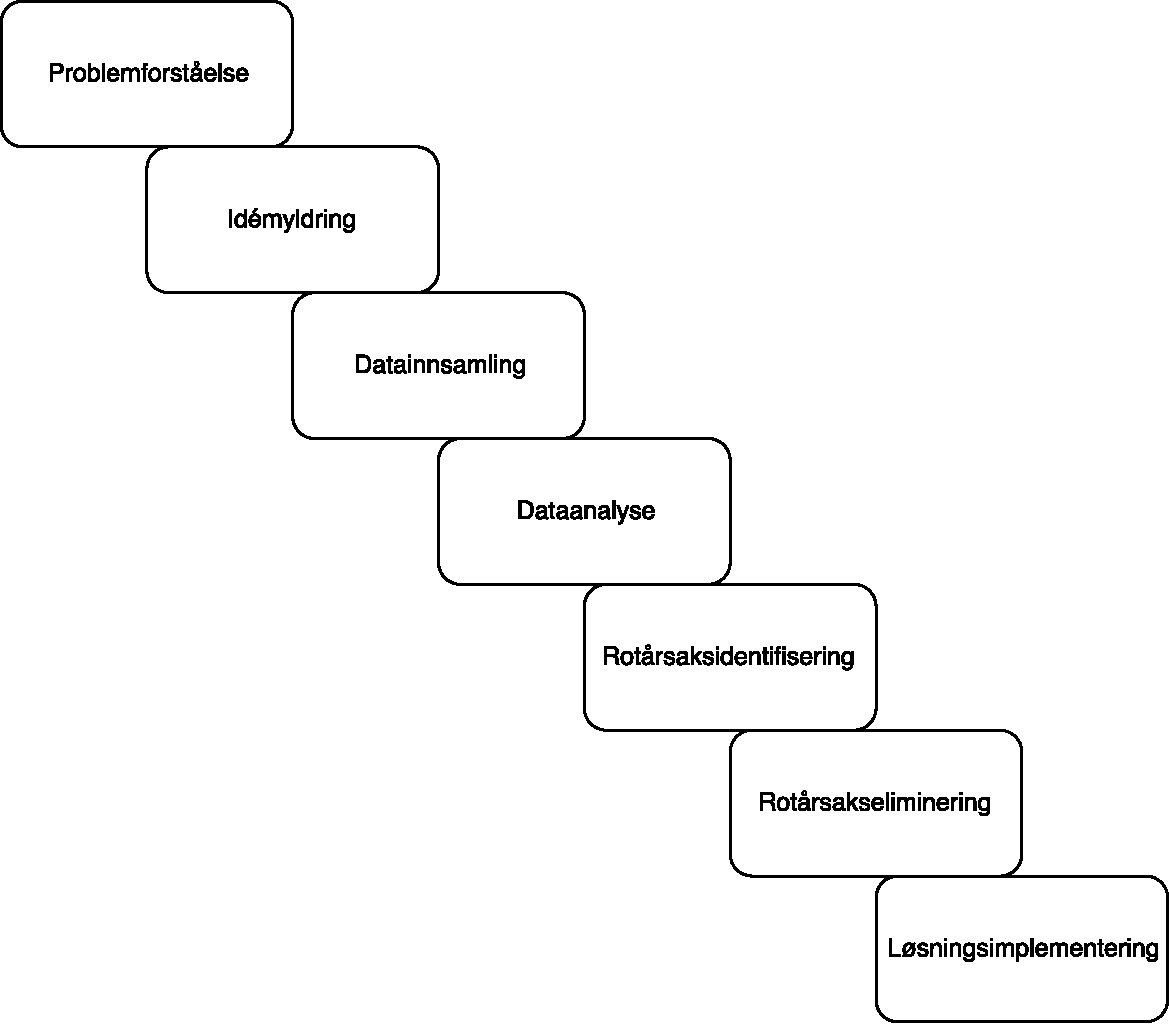
\includegraphics[scale=0.4]{prosess}
    \caption[RCA-prosess]{De syv fasene i rotårsaksanalyseprosessen}
    \label{fig:prosess}
\end{figure}
\subsection{Problemforståelse}
Problemforståelse går ut på å få en solid forståelse for problemet en ønsker å løse. Det kan også hjelpe med å skape enighet rundt hva problemet egentlig omfatter. Det er også viktig for å passe på at ressursene som benyttes for analysen brukes effektivt videre. 

Verktøyene vi anbefaler til denne fasen er: 
\begin{description}
    \item[Kritiske hendelser] Kritiske hendeleser er et godt verktøy å bruke når man har mye data, som kan gi et innblikk i hva som går galt. Innen IT pleier en å logge mye, noe som gir mye data.
\end{description}

\subsection{Idémyldring}
Målet med idémyldring er å generere så mange idéer som mulig om et gitt emne. I rotårsaksanalyse er målet stort sett å generere en liste over problemområder som kan forbedres, identifisere mulige konsekvenser, generere en liste over mulige årsaker til problemet og oppmuntre til å tenke på løsninger som kan eliminere problemet. 

Verktøyene vi anbefaler til denne fasen er:
\begin{description}
    \item[Idémyldring] Idémyldring gir mange idéer om mulige rotårsaker. Hvis det er noen som dominerende i gruppen som gjennomfører idémyldringen, burde idéskriving benyttes.
    \item[Nominell gruppe teknikk] Dette verktøyet gir en liste over hva en burde prioritere mest i datainnsamling for å gi ett godt datagrunnlag for å finne rotårsaken. Ved å bruke resultatene fra idémyldingen, får en prioritert disse idéene. 
\end{description}

\subsection{Datainnsamling}
Ustrukturert og tilfeldig problemløsning har en tendens til å bli svært unøyaktig. Strukturert rotårsaksanalyse gir derimot et godt grunnlag for blant annet datainnsamlingen, som er en av de sentrale fasene i prosessen.

\begin{description}
    \item[Sampling] Sampling er et godt verktøy for å begrense datainnsamling til de relevante gruppene. 
    \item[Spørreundersøkelser] Spørreundersøkelser er et godt verktøy for å få data fra de berørte personene. 
\end{description}

\subsection{Dataanalyse}
I denne fasen blir dataene analysert og visualisert. Hovedmålet er å avklare mulige rotårsaker som har innvirkning på problemet, og hvilke av de som har størst innflytelse. Under beskrives de ulike verktøyene som ble brukt for å analysere dataene.

Verktøyene vi anbefaler til denne fasen er:
\begin{description}
    \item[Histogram] Histogram fungerer veldig godt for å skape en visuell forståelse av dataene, som kan gjøre det lettere å se korrelasjoner mellom variabler. Det gir også en tilfredstillende fremstilling av dataen. 
    \item[Affinitetsdiagram] Affinitetsdiagram passer veldig godt med spørreundersøkelser, der det er kortsvar- eller langsvaroppgaver. Det gir mulighet for å gruppere svarene etter innhold i svarene. 
    \item[Statistisk analyse] Statistisk analyse er ikke i boken, men er noe analyse metode som fungerer veldig godt for å se korrelasjoner. Dette fungerer også ved å se på signifikansen.
\end{description}

\subsection{Rotårsaksidentifisering}
De foregående fasene skal ha generert en liste over mulige rotårsaker og målet i denne fasen er å identifisere de faktiske årsakene. Det kan kreve flere iterasjoner for å finne rotårsaken(e). 

Verktøyene vi anbefaler til denne fasen er:
\begin{description}
    \item[Årsak-virkning diagram] Som årsak-virkning anbefaler vi å benytte fiskebeindiagram. Ved å bruke fiskebeindiagram får en en visuell fremstilling av rotårsaken til problemet. 
    \item[5 Whys] Hvis det er mistanke om høyere årsaker bak de identifiserte årsakene kan 5 whys gi en bekreftelse på om årsakene identifisert er faktisk rotårsak og ikke lav-nivå årsaker. 
    \item[Feiltreanalyse] 
\end{description}

\subsection{Rotårsakseliminering}
Denne fasen innebærer å komme med mulige løsninger til problemet for å eliminere rotårsaken. Boken til Fagerhaug og Andersen \cite{RCA} beskriver to mulige tilnærminger til denne fasen. En tilnærming for å stimulere kreativitet når man leter etter løsninger, og en for å konstruere og utvikle løsninger.

Verktøyene vi anbefaler til denne fasen er:
\begin{description}
    \item[De seks tenkehatter]
    \item[SIT] 
\end{description}
Bruk SIT - så sant det ikke er fysiske krav. Da kanskje bruke TRIZ. 
Krever kreativ løsning, bruk 6 tenkehatter

\subsection{Løsningsimplementering}
I den siste fasen er målet å implementere løsningene som ble funnet i foregående fase. Implementeringen inkluderer blant annet organisering, utvikling av en implementeringsplan, skape et konsensus om de nødvendige endringene og selvfølgelig implementeringen. Implementeringen av løsningen kan sies å være en suksess når symptomene forsvinner. 

Verktøyene vi anbefaler til denne fasen er:
\begin{description}
    \item[Trediagram] Trediagram fungerer veldig bra for å lage en plan over hva som må gjøres for at tiltaket skal bli implementert. 
\end{description}
I dette steget er de ikke nødvendig å bruke noe verktøy, men det kan være lurt å benytte trediagram for å få en plan over løsningimplementering.


\chapter{Konklusjon}
\label{kap:konklusjon}
Rotårsaksanalyse er ikke en standardisert metodikk. Det finnes mye som blir kalt rotårsaksanalyse, men dette prosjektet tok utgangspunkt i metodikken til Fagerhaug og Andersen \cite{RCA}. Hovedformålet med prosjektet var å undersøke om rotårsaksanalysemetodikk har bruksområder innen informasjonssikkerhet. Tilnærmingen var gjennom tre caser der målet var å finne rotårsaken og gi forslag til tiltak som kunne eliminere disse. Ut fra disse kriteriene ble det definert noen forskningsspørsmål. Tre av de var å finne rotårsaken til: ulovlig fildeling ved universitetsnettet, kompromitterte kontoer ved NTNU og misbruk av NTNU sine ressurser til utvinning av kryptovaluta. De siste forskningsspørsmålene gikk på å vurdere hvor godt rotårsaksanalyse fungerer innen informasjonssikkerhet, om det er lønnsomt å bruke det og hvilke verktøy som fungerer best innen informasjonssikkerhet. 
\newline

\noindent Rotårsaken til ulovlig fildeling viste seg i hovedsak å være tilgjengeligheten, eller mangelen på den. En mindre årsak var at de følte ikke tjenestene var verdt det de måtte betale. En siste årsak ble funnet, nemlig at håndhevingen og kommuniseringen av lovene knyttet til ulovlig fildeling er utilstrekkelig og blir ikke prioritert. Tiltak vi har foreslått for å løse dette problemet er å tilby produkter fra selskaper som sender mest notifikasjoner om brudd på opphavsrett, å ha et kurs for studenter i bruk av universitetets nettverk, at Sit regelrett bytter ISP slik at problemet blir overført til andre og tilslutt at alt materiale blir tilgengelig på ett sted. Det siste tiltaket er urealistisk, men vil fjerne rotårsaken helt. 
\newline

\noindent Når det kommer til kompromitterte kontoer konkluderer vi med at både gjenbruk av kredentialier og phishing er de største rotårsakene. I tillegg resulterte analysen også i at folk som har blitt kompromittert kjenner svært dårlig til styrende dokumenter på IT, informasjonssikkerhet og behandling av autentiseringsdata. Vi kom også frem til at det var utilstrekkelig tilgangskontroll på brukerkontoene da vi mener brukernavn og passord ikke er nok. For å løse dette anbefaler vi en rekke tiltak, som inkluderer: en bevisstgjørelseskampanje for god e-postskikk og behandling av autentiseringsdata, krav om strengere passordkontroll, implementere 2-faktor autentisering, klarere enheter for en viss periode gjennom 2-faktor autentisering og informering om innlogginger fra andre maskiner, utbedre IT-reglementet til å inkludere retningslinjer og krav, og til slutt å anbefale eller pålegge brukere å benytte seg av passordmanager. Av disse anbefaler vi spesielt å klarere enheter med 2-faktor autentisering i en viss periode av gangen, og i tillegg gi informasjon når det logges på fra en ny maskin. 
\newline

\noindent På caset om misbruk av ressurser til kryptoutvinning kom vi frem til at rotårsaken av en blanding av uklarheter i IT-reglementet angående kryptoutvinning og at Seksjon for Digital Sikkerhet ikke har ressurser til å prioritere problemet. For å løse problemet anbefaler vi å gjennomføre en informasjonskampanje om kommersielt misbruk av NTNU sin infrastruktur, gjøre IT-reglementet klarere på misbruk av ressursene spesifikt når det kommer til kryptoutvinning, DNS blokkering av kryptoforespørsler og tilsutt øke antall personell i seksjonen, enten i form av faste ansatte eller flere bacheloroppgaver. 
\newline

\noindent Basert på erfaring fra utføringen av casestudiene kan vi konkludere med at rotårsaksanalyse fungerer godt innen informasjonssikkerhet. Dette kommer selvfølgelig helt an på hvor god datainnsamlingen er. Det kommer også an på hva slags case det benyttes på, da noen har en rotårsak som ikke kan fjernes. Rotårsaksanalyse gir også mulighet for forskjellige resultater da rotårsaken ofte ikke er den du ser med første øyekast. For å konkludere endelig med hvor godt det fungerer må tiltakene innføres. Deretter kan man se om de fjerner problemet eller ikke. 
\newline

\noindent Rotårsaksanalyse er en strukturert problemløsningsmetode som egner seg godt ved lengre tidsbruk, men også helt greit over kortere tid. Det er spesielt viktig å ikke velge et for komplisert case hvis det er liten tid, da rotårsaksanalysen kan fort bli oppstykket og uferdig. Den største styrken ved rotårsaksanalyse er evnen den gir til å sette seg dypt inn i en problemstilling. Dette er nyttig uansett om det er mulig å fjerne rotårsaken eller ikke. I visse situasjoner kan det være mer fordelaktig å utføre en risiko- og sårbarhetsanalyse, men da kan du miste den dype forståelsen av bakgrunnen til problemet. Tidsbruken gjenspeilet stort sett resultatene vi fikk. Inkludert har vi også en veiledning som skal hjelpe med å veilede personer som ønsker å utføre rotårsaksanalyser på caser som omhandler informasjonssikkerhet. Dette dokumentet beskriver hvilke verktøy en bør bruke i ulike sammenhenger. Veiledningen finnes i kapittel \ref{kap:veiledning-RCA}. 

\section{Videre arbeid}
Vi anbefaler at videre arbeid blir å gjennomgå tiltaksforslagene våre, og se om noen av disse er fornuftige å implementere, samt om de er verdt kostnadene. Ulovlig fildeling på universitetnettet er et veldig vanskelig problem å fjerne rotårsaken til, siden tilgjengelighet er den store drivkraften bak nedlasting. Det kan også være nyttig å undersøke hvilke opphavsrettshavere som sender notifikasjoner, for å se om universitetet kan tilby tjenester hvis de fleste kommer fra ett sted. Videre arbeid kan også inkludere en risikoanalyse for å underbygge problemstillingen knyttet til ulovlig fildeling på universitetsnettet. 

Siden vi bare tok et sample fra de som tidligere hadde blitt kompromittert kan det være interessant å undersøke hele NTNU når det kommer til passordvaner, e-post, kjennskap til retningslinjer osv. Deretter kan resultatene sammenlignes og se om det er noen forskjeller som bør tas i betraktning. Annet videre arbeid kan være å undersøke keylogging som en mulig årsak til kompromitterte kontoer. Vi gikk ikke så mye inn på det i denne rapporten, men det kan være interessant å se på i forlengelse av ondsinnet programvare. 

Siden datagrunnlaget vårt var noe snevert på case 3 kan det være interessant å hente inn mer data, for å se om det er andre underliggende rotårsaker vi ikke fant. Retningslinjer for bruk utvinning av kryptovaluta burde i teorien få alle ansatte eller studenter til å slutte å utvinne. Men de er mennesker så det kan være greit å se etter flere tekniske løsninger som hinder uautorisert utvinning av kryptovaluta. 

Siden estimatene på nytten i kostnad-nytte-analysen var vage, kan videre arbeid være å utføre en ny kostnad-nytte-analyse basert på mer konkrete verdier, etter tiltakene er implementert. 

videre arbeid på veiledninger
Veilederen inneholder kun fremgangsmåte til verktøy vi har gjennomgåt. Derfor vil videre arbeid innen veilederen være å utføre nye rotårsaksanalyser som tar for seg nye verktøy og se hvordan de fungerer innen informasjonssikkerhet. Hvis de fungerer godt, må de innarbeides inn i veilederen med en stegvis forklaringsmetode av verktøyet.
%\input{main/}



\bibliographystyle{ntnuthesis/ntnubachelorthesis}
\bibliography{main/referanser}

\appendix %after this line all chapters will have leters instead of numbers
\chapter{Spørreundersøkelse case 1}
\label{sporreundersokelser}
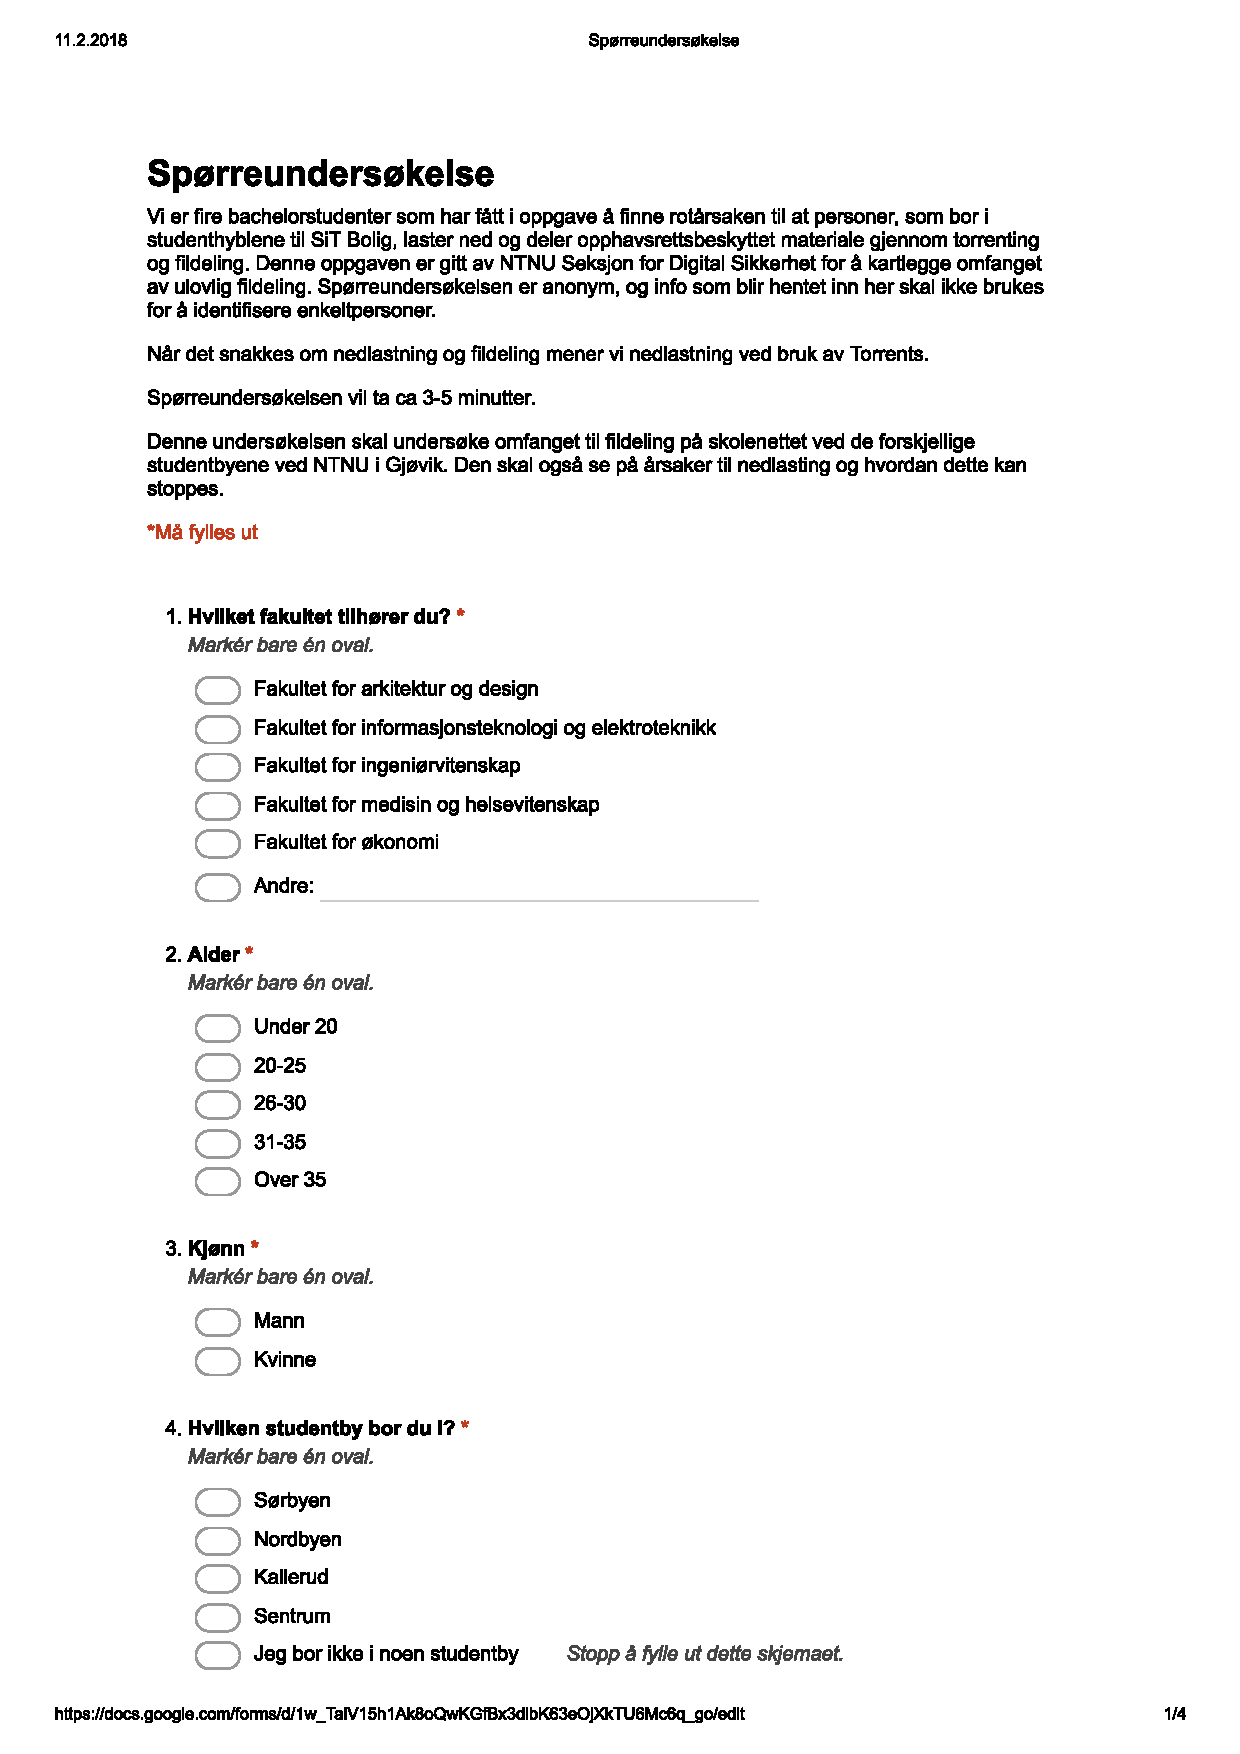
\includepdf[pages={1-4}]{case_1/bilder/case1_sporreundersokelse}
\label{undersokelse}

\chapter{Spørreundersøkelse case 2 (norsk og engelsk)}
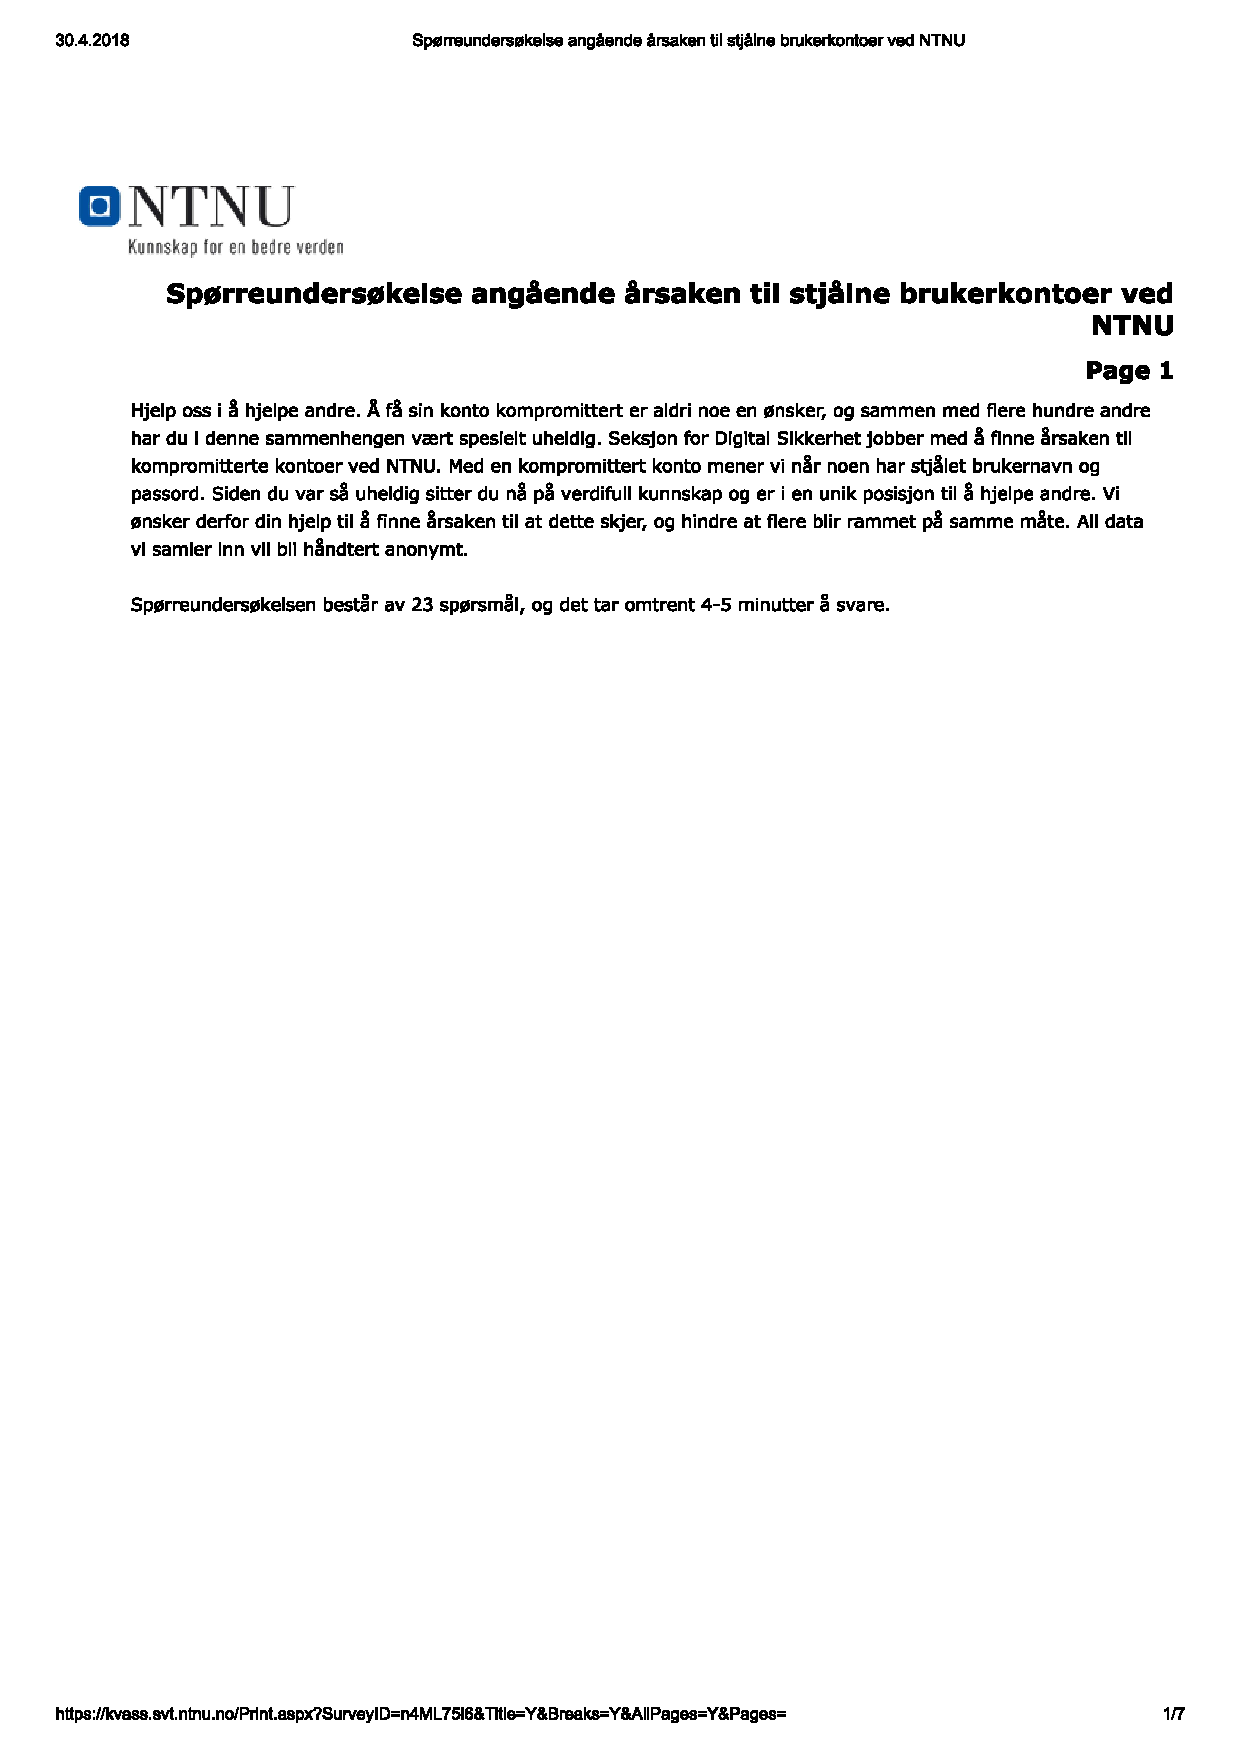
\includepdf[pages={1-6}]{case_2/bilder/sporreundersokelse_norsk.pdf}
\label{undersokelse_norsk}

\includepdf[pages={1-6}]{case_2/bilder/sporreundersokelse_engelsk.pdf}
\label{undersokelse_engelsk}

\chapter{Spørreundersøkelse case 2 resultater (norsk og engelsk)}
\includepdf[pages={1-4}]{case_2/bilder/sporreundersokelse_norsk_resultater.pdf}
\label{undersokelse_norsk_resultater}

\includepdf[pages={1-4}]{case_2/bilder/sporreundersokelse_engelsk_resultater.pdf}
\label{undersokelse_engelsk_resultater}
\chapter{Vedlegg: Plakat}
\label{plakat}
\begin{figure}[H]
    \centering
    \includegraphics[scale=0.25]{case_1/bilder/plakat.pdf}
    \caption[Promoteringsplakat]{Plakat som ble brukt i forbindelse med promotering av spørreundersøkelsen}
    \label{fig:plakat}
\end{figure}
\chapter{Vedlegg: Frekvenstabeller case 1}
\label{frekvens}

% Table generated by Excel2LaTeX from sheet 'Ark1'
\begin{table}[htbp]
  \centering
    \begin{tabular}{|l|r|r|r|l|}
    \hline
    \multicolumn{5}{|p{30em}|}{\textcolor[rgb]{ .6,  .2,  0}{\textbf{\begin{center}Kjønn\end{center}}}} \\
    \hline
    \textcolor[rgb]{ .2,  .2,  .6}{} & \multicolumn{1}{p{5.355em}|}{\textcolor[rgb]{ .2,  .2,  .6}{Frequency}} & \multicolumn{1}{p{5.355em}|}{\textcolor[rgb]{ .2,  .2,  .6}{Percent}} & \multicolumn{1}{p{5.355em}|}{\textcolor[rgb]{ .2,  .2,  .6}{Valid Percent}} & \multicolumn{1}{p{5.355em}|}{\textcolor[rgb]{ .2,  .2,  .6}{Cumulative Percent}} \\
    \hline
    \textcolor[rgb]{ .2,  .2,  .6}{Kvinne} & \textcolor[rgb]{ .6,  .2,  0}{27} & \textcolor[rgb]{ .6,  .2,  0}{27.8} & \textcolor[rgb]{ .6,  .2,  0}{27.8} & \multicolumn{1}{r|}{\textcolor[rgb]{ .6,  .2,  0}{27.8}} \\
    \hline
    \textcolor[rgb]{ .2,  .2,  .6}{Mann}  & \textcolor[rgb]{ .6,  .2,  0}{70} & \textcolor[rgb]{ .6,  .2,  0}{72.2} & \textcolor[rgb]{ .6,  .2,  0}{72.2} & \multicolumn{1}{r|}{\textcolor[rgb]{ .6,  .2,  0}{100.0}} \\
    \hline
    \textcolor[rgb]{ .2,  .2,  .6}{Total} & \textcolor[rgb]{ .6,  .2,  0}{97} & \textcolor[rgb]{ .6,  .2,  0}{100.0} & \textcolor[rgb]{ .6,  .2,  0}{100.0} & \textcolor[rgb]{ .6,  .2,  0}{} \\
    \hline
    \end{tabular}%
  \caption{Frekvenstabell av kjønn}
  \label{tab:kjonn}%
\end{table}%

\begin{table}[htbp]
  \centering
    \begin{tabular}{|l|r|r|r|l|}
    \hline
    \multicolumn{5}{|p{30em}|}{\textcolor[rgb]{ .6,  .2,  0}{\textbf{\begin{center}Alder\end{center}}}} \\
    \hline
    \textcolor[rgb]{ .2,  .2,  .6}{} & \multicolumn{1}{p{5.355em}|}{\textcolor[rgb]{ .2,  .2,  .6}{Frequency}} & \multicolumn{1}{p{5.355em}|}{\textcolor[rgb]{ .2,  .2,  .6}{Percent}} & \multicolumn{1}{p{5.355em}|}{\textcolor[rgb]{ .2,  .2,  .6}{Valid Percent}} & \multicolumn{1}{p{5.355em}|}{\textcolor[rgb]{ .2,  .2,  .6}{Cumulative Percent}} \\
    \hline
    \textcolor[rgb]{ .2,  .2,  .6}{Under 20} & \textcolor[rgb]{ .6,  .2,  0}{9} & \textcolor[rgb]{ .6,  .2,  0}{9.3} & \textcolor[rgb]{ .6,  .2,  0}{9.3} & \multicolumn{1}{r|}{\textcolor[rgb]{ .6,  .2,  0}{9.3}} \\
    \hline
    \textcolor[rgb]{ .2,  .2,  .6}{20-25}  & \textcolor[rgb]{ .6,  .2,  0}{72} & \textcolor[rgb]{ .6,  .2,  0}{74.2} & \textcolor[rgb]{ .6,  .2,  0}{74.2} & \multicolumn{1}{r|}{\textcolor[rgb]{ .6,  .2,  0}{83.5}} \\
    \hline
    \textcolor[rgb]{ .2,  .2,  .6}{26-30} & \textcolor[rgb]{ .6,  .2,  0}{11} & \textcolor[rgb]{ .6,  .2,  0}{11.3} & \textcolor[rgb]{ .6,  .2,  0}{11.3} & \multicolumn{1}{r|}{\textcolor[rgb]{ .6,  .2,  0}{94.9}} \\
    \hline
    \textcolor[rgb]{ .2,  .2,  .6}{31-35} & \textcolor[rgb]{ .6,  .2,  0}{4} & \textcolor[rgb]{ .6,  .2,  0}{4.1} & \textcolor[rgb]{ .6,  .2,  0}{4.1} & \multicolumn{1}{r|}{\textcolor[rgb]{ .6,  .2,  0}{99.0}} \\
    \hline
    \textcolor[rgb]{ .2,  .2,  .6}{Over 35} & \textcolor[rgb]{ .6,  .2,  0}{1} & \textcolor[rgb]{ .6,  .2,  0}{1.0} & \textcolor[rgb]{ .6,  .2,  0}{1.0} & \multicolumn{1}{r|}{\textcolor[rgb]{ .6,  .2,  0}{100.0}} \\
    \hline
    \textcolor[rgb]{ .2,  .2,  .6}{Total} & \textcolor[rgb]{ .6,  .2,  0}{97} & \textcolor[rgb]{ .6,  .2,  0}{100.0} & \textcolor[rgb]{ .6,  .2,  0}{100.0} & \multicolumn{1}{r|}{\textcolor[rgb]{ .6,  .2,  0}{}} \\
    \hline
    \end{tabular}%
  \caption{Frekvenstabell av alder}
  \label{tab:alder}%
\end{table}%

\begin{table}[htbp]
  \centering
    \begin{tabular}{|l|r|r|r|l|}
    \hline
    \multicolumn{5}{|p{30em}|}{\textcolor[rgb]{ .6,  .2,  0}{\textbf{\begin{center}Studentby\end{center}}}} \\
    \hline
    \textcolor[rgb]{ .2,  .2,  .6}{} & \multicolumn{1}{p{5.355em}|}{\textcolor[rgb]{ .2,  .2,  .6}{Frequency}} & \multicolumn{1}{p{5.355em}|}{\textcolor[rgb]{ .2,  .2,  .6}{Percent}} & \multicolumn{1}{p{5.355em}|}{\textcolor[rgb]{ .2,  .2,  .6}{Valid Percent}} & \multicolumn{1}{p{5.355em}|}{\textcolor[rgb]{ .2,  .2,  .6}{Cumulative Percent}} \\
    \hline
    \textcolor[rgb]{ .2,  .2,  .6}{Kallerud} & \textcolor[rgb]{ .6,  .2,  0}{49} & \textcolor[rgb]{ .6,  .2,  0}{50.5} & \textcolor[rgb]{ .6,  .2,  0}{50.5} & \multicolumn{1}{r|}{\textcolor[rgb]{ .6,  .2,  0}{50.5}} \\
    \hline
    \textcolor[rgb]{ .2,  .2,  .6}{Nordbyen}  & \textcolor[rgb]{ .6,  .2,  0}{13} & \textcolor[rgb]{ .6,  .2,  0}{13.4} & \textcolor[rgb]{ .6,  .2,  0}{13.4} & \multicolumn{1}{r|}{\textcolor[rgb]{ .6,  .2,  0}{63.9}} \\
    \hline
    \textcolor[rgb]{ .2,  .2,  .6}{Sentrum} & \textcolor[rgb]{ .6,  .2,  0}{11} & \textcolor[rgb]{ .6,  .2,  0}{11.3} & \textcolor[rgb]{ .6,  .2,  0}{11.3} & \multicolumn{1}{r|}{\textcolor[rgb]{ .6,  .2,  0}{75.3}} \\
    \hline
    \textcolor[rgb]{ .2,  .2,  .6}{Sørbyen} & \textcolor[rgb]{ .6,  .2,  0}{24} & \textcolor[rgb]{ .6,  .2,  0}{24.7} & \textcolor[rgb]{ .6,  .2,  0}{24.7} & \multicolumn{1}{r|}{\textcolor[rgb]{ .6,  .2,  0}{100.0}} \\
    \hline
    \textcolor[rgb]{ .2,  .2,  .6}{Total} & \textcolor[rgb]{ .6,  .2,  0}{97} & \textcolor[rgb]{ .6,  .2,  0}{100.0} & \textcolor[rgb]{ .6,  .2,  0}{100.0} & \multicolumn{1}{r|}{\textcolor[rgb]{ .6,  .2,  0}{}} \\
    \hline
    \end{tabular}%
  \caption{Frekvenstabell av studentby}
  \label{tab:studentby}%
\end{table}%

\begin{table}[htbp]
  \centering
    \begin{tabular}{|p{5.355em}|r|r|r|l|}
    \hline
    \multicolumn{5}{|p{30em}|}{\textcolor[rgb]{ .6,  .2,  0}{\textbf{\begin{center}Fakultet\end{center}}}} \\
    \hline
    \multicolumn{1}{|r|}{\textcolor[rgb]{ .2,  .2,  .6}{}} & \multicolumn{1}{p{5.355em}|}{\textcolor[rgb]{ .2,  .2,  .6}{Frequency}} & \multicolumn{1}{p{5.355em}|}{\textcolor[rgb]{ .2,  .2,  .6}{Percent}} & \multicolumn{1}{p{5.355em}|}{\textcolor[rgb]{ .2,  .2,  .6}{Valid Percent}} & \multicolumn{1}{p{5.355em}|}{\textcolor[rgb]{ .2,  .2,  .6}{Cumulative Percent}} \\
    \hline
    \textcolor[rgb]{ .2,  .2,  .6}{Fakultet for arkitektur og design} & \textcolor[rgb]{ .6,  .2,  0}{15} & \textcolor[rgb]{ .6,  .2,  0}{15.5} & \textcolor[rgb]{ .6,  .2,  0}{15.5} & \multicolumn{1}{r|}{\textcolor[rgb]{ .6,  .2,  0}{15.5}} \\
    \hline
    \textcolor[rgb]{ .2,  .2,  .6}{Fakultet for informasjonsteknologi og elektroteknikk} & \textcolor[rgb]{ .6,  .2,  0}{52} & \textcolor[rgb]{ .6,  .2,  0}{53.6} & \textcolor[rgb]{ .6,  .2,  0}{53.6} & \multicolumn{1}{r|}{\textcolor[rgb]{ .6,  .2,  0}{69.1}} \\
    \hline
    \textcolor[rgb]{ .2,  .2,  .6}{Fakultet for ingeniørvitenskap} & \textcolor[rgb]{ .6,  .2,  0}{13} & \textcolor[rgb]{ .6,  .2,  0}{13.4} & \textcolor[rgb]{ .6,  .2,  0}{13.4} & \multicolumn{1}{r|}{\textcolor[rgb]{ .6,  .2,  0}{82.5}} \\
    \hline
    \textcolor[rgb]{ .2,  .2,  .6}{Fakultet for medisin og helsevitenskap} & \textcolor[rgb]{ .6,  .2,  0}{11} & \textcolor[rgb]{ .6,  .2,  0}{11.3} & \textcolor[rgb]{ .6,  .2,  0}{11.3} & \multicolumn{1}{r|}{\textcolor[rgb]{ .6,  .2,  0}{93.8}} \\
    \hline
    \textcolor[rgb]{ .2,  .2,  .6}{Fakultet for økonomi} & \textcolor[rgb]{ .6,  .2,  0}{6} & \textcolor[rgb]{ .6,  .2,  0}{6.2} & \textcolor[rgb]{ .6,  .2,  0}{6.2} & \multicolumn{1}{r|}{\textcolor[rgb]{ .6,  .2,  0}{100.0}} \\   
    \hline
    \textcolor[rgb]{ .2,  .2,  .6}{Total} & \textcolor[rgb]{ .6,  .2,  0}{97} & \textcolor[rgb]{ .6,  .2,  0}{100.0} & \textcolor[rgb]{ .6,  .2,  0}{100.0} & \textcolor[rgb]{ .6,  .2,  0}{} \\
    \hline
    \end{tabular}%
  \caption{Frekvenstabell av fakultet}
  \label{tab:fakultet}%
\end{table}%

\chapter{Vedlegg: Diverse histogrammer fra case 1}
\label{vedlegg:histogrammer}

\begin{figure}[H]
    \centering
    \includegraphics[scale=0.45]{case_1/bilder/IT_lasterned.pdf}
    \caption[Forskjellen mellom fakultetene og om de laster ned]{Forholdet mellom IT studier og andre når det kommer til nedlasting}
    \label{fig:IT-lasterned}
\end{figure}

\begin{figure}[H]
    \centering
    \includegraphics[scale=0.45]{case_1/bilder/reglement_lasterned.pdf}
    \caption[Forholdet mellom kjennskap til IT reglement og om de laster ned]{Forholdet mellom kjennskap til IT reglement og om en laster ned}
    \label{fig:reglement-lasterned}
\end{figure}

\begin{figure}[H]
    \centering
    \includegraphics[scale=0.45]{case_1/bilder/reglement_fakultet.pdf}
    \caption[Forskjellen mellom fakultetene og kjennskap til IT reglement]{Hvor godt kjennskap de ulike fakultetene har med IT reglementet}
    \label{fig:reglement-fakultet}
\end{figure}

\begin{figure}[H]
    \centering
    \includegraphics[scale=0.45]{case_1/bilder/antalltorrents.pdf}
    \caption[Antall torrents som blir lastet ned hver måned]{Hvor mange torrents folk laster ned i løpet av en måned}
    \label{fig:antalltorrents}
\end{figure}

\chapter{Vedlegg: Diverse histogrammer fra case 2}
\begin{figure}[H]
    \centering
    \includegraphics[scale=0.5]{case_2/bilder/spss/oppdaget_virus.pdf}
    \caption[Oppdaget virus]{Oversikt over hvor mange som oppdaget virus på datamaskinen}
    \label{fig:oppdaget-virus}
\end{figure}

\begin{figure}[H]
    \centering
    \includegraphics[scale=0.5]{case_2/bilder/spss/passord_deling.pdf}
    \caption[Oversikt over passorddeling]{Viser hvor mange som har delt sitt NTNU passord før}
    \label{fig:passord-deling}
\end{figure}

\begin{figure}[H]
    \centering
    \includegraphics[scale=0.5]{case_2/bilder/spss/tilfeldig_passord.pdf}
    \caption[Hvor mange som bruker tilfeldig passord]{Viser hvor mange som bruker tilfeldig sammensatt passord}
    \label{fig:tilfeldig-passord}
\end{figure}

\begin{figure}[H]
    \centering
    \includegraphics[scale=0.5]{case_2/bilder/spss/pass_manager.pdf}
    \caption[Hvor mange som bruker passordmanager]{Viser hvor mange som bruker passord manager}
    \label{fig:passord-manager}
\end{figure}
\chapter{Vedlegg: Statistisk analyse case 2}
\label{vedlegg:statanalys}

\section*{År ved NTNU mot bevissthet på sikkerhet og kjennskap til retningslinjer}
\label{aarvedNTNU-mot-bevissthetogkjennskap}
\begin{figure}[H]
    \centering
    \includegraphics[scale=0.7]{case_2/bilder/spss/anova_ttest/ansiennitet_bevissthetogkjennskap_descriptive_1.pdf}
    \caption[Antall år ved NTNU mot bevissthet og kjennskap descriptive 1]{Descriptive av tid ved NTNU mot bevissthet på sikkerhet og kjennskap til retningslinjer, del 1}
    \label{fig:ansiennitet-bevissthetogkjennskap-descriptive-1}
\end{figure}

\begin{figure}[H]
    \centering
    \includegraphics[scale=0.7]{case_2/bilder/spss/anova_ttest/ansiennitet_bevissthetogkjennskap_descriptive_2.pdf}
    \caption[Antall år ved NTNU mot bevissthet og kjennskap descriptive 2]{Descriptive av tid ved NTNU mot bevissthet på sikkerhet og kjennskap til retningslinjer, del 2}
    \label{fig:ansiennitet-bevissthetogkjennskap-descriptive-2}
\end{figure}

\begin{figure}[H]
    \centering
    \includegraphics[scale=0.7]{case_2/bilder/spss/anova_ttest/ansiennitet_bevissthetogkjennskap_anova.pdf}
    \caption[Antall år ved NTNU mot bevissthet og kjennskap ANOVA]{Anova av tid ved NTNU mot bevissthet på sikkerhet og kjennskap til retningslinjer}
    \label{fig:ansiennitet-bevissthetogkjennskap-anova}
\end{figure}

\begin{figure}[H]
    \centering
    \includegraphics[scale=0.7]{case_2/bilder/spss/anova_ttest/ansiennitet_bevissthetogkjennskap_posthoc_1.pdf}
    \caption[Antall år ved NTNU mot bevissthet og kjennskap post-hoc 1]{Post-hoc av tid ved NTNU mot bevissthet på sikkerhet og kjennskap til retningslinjer, del 1}
    \label{fig:ansiennitet-bevissthetogkjennskap-posthoc-1}
\end{figure}

\begin{figure}[H]
    \centering
    \includegraphics[scale=0.7]{case_2/bilder/spss/anova_ttest/ansiennitet_bevissthetogkjennskap_posthoc_2.pdf}
    \caption[Antall år ved NTNU mot bevissthet og kjennskap post-hoc 2]{Post-hoc av tid ved NTNU mot bevissthet på sikkerhet og kjennskap til retningslinjer, del 2}
    \label{fig:ansiennitet-bevissthetogkjennskap-posthoc-2}
\end{figure}

\section*{Kjønn mot bevissthet på sikkerhet og kjennskap til retningslinjer}
\label{kjonn-mot-bevissthetogkjennskap}
\begin{figure}[H]
    \centering
    \includegraphics[scale=0.8]{case_2/bilder/spss/anova_ttest/kjonn_bevissthetogkjennskap_groupstats.pdf}
    \caption[Gruppestatistikk av kjønn mot bevissthet på sikkerhet og kjennskap til retningslinjer]{Gruppestatistikk av kjønn mot bevissthet på sikkerhet og kjennskap til retningslinjer}
    \label{fig:kjonn-bevissthetogkjennskap-groupstats}
\end{figure}

\begin{figure}[H]
    \centering
    \includegraphics[scale=0.4]{case_2/bilder/spss/anova_ttest/kjonn_bevissthetogkjennskap_ttest.pdf}
    \caption[T-test av kjønn mot bevissthet på sikkerhet og kjennskap til retningslinjer]{Independent t-test av kjønn mot bevissthet på sikkerhet og kjennskap til retningslinjer}
    \label{fig:kjonn-bevissthetogkjennskap-ttest}
\end{figure}
\chapter{Vedlegg: Flytdiagrammer for verktøyvalg}
\label{flytdiagrammer-verktoyvalg}

\begin{figure}[H]
    \centering
    \includegraphics[scale=0.35]{main/bilder/verktoyvalg/verktoyvalg_problemforstaelse.pdf}
    \caption[Verktøyvalg for problemforståelse]{De ulike verktøyene boken anbefaler i problemforståelse ut fra spesifikke kriterier}
    \label{fig:verktoyvalg-problemforstaelse}
\end{figure}

\begin{figure}[H]
    \centering
    \includegraphics[scale=0.65]{main/bilder/verktoyvalg/verktoyvalg_idemyldring.pdf}
    \caption[Verktøyvalg for idémyldring]{De ulike verktøyene boken anbefaler i idémyldring ut fra spesifikke kriterier}
    \label{fig:verktoyvalg-idemyldring}
\end{figure}

\begin{figure}[H]
    \centering
    \includegraphics[scale=0.65]{main/bilder/verktoyvalg/verktoyvalg_datainnsamling.pdf}
    \caption[Verktøyvalg for datainnsamling]{De ulike verktøyene boken anbefaler i datainnsamling ut fra spesifikke kriterier}
    \label{fig:verktoyvalg-datainnsamling}
\end{figure}

\begin{figure}[H]
    \centering
\includegraphics[scale=0.65]{main/bilder/verktoyvalg/verktoyvalg_dataanalyse.pdf}
    \caption[Verktøyvalg for dataanalyse]{De ulike verktøyene boken anbefaler i dataanalyse ut fra spesifikke kriterier}
    \label{fig:verktoyvalg-dataanalyse}
\end{figure}

\begin{figure}[H]
    \centering
    \includegraphics[scale=0.65]{main/bilder/verktoyvalg/verktoyvalg_rotarsaksidentifisering.pdf}
    \caption[Verktøyvalg for rotårsaksidentifisering]{De ulike verktøyene boken anbefaler i rotårsaksidentifisering ut fra spesifikke kriterier}
    \label{fig:verktoyvalg-rotarsaksidentifisering}
\end{figure}

\begin{figure}[H]
    \centering
    \includegraphics[scale=0.65]{main/bilder/verktoyvalg/verktoyvalg_rotarsakseliminering.pdf}
    \caption[Verktøyvalg for rotårsakseliminering]{De ulike verktøyene boken anbefaler i rotårsakseliminering ut fra spesifikke kriterier}
    \label{fig:verktoyvalg-rotarsakseliminering}
\end{figure}

\begin{figure}[H]
    \centering
    \includegraphics[scale=0.65]{main/bilder/verktoyvalg/verktoyvalg_losningsimplementering.pdf}
    \caption[Verktøyvalg for løsningsimplementering]{De ulike verktøyene boken anbefaler i løsningsimplementering ut fra spesifikke kriterier}
    \label{fig:verktoyvalg-losningsimplementering}
\end{figure}

\end{document}
